\section{Introduction}

In the previous chapter, we modelled the $y$-direction as invariant. This chapter builds on the last, by allowing for an $\exp(ik_y y)$  $y$-dependence. We will see that this enables mode conversion and a phenomenon called resonant absorption to occur.
Resonant absorption is a process where magnetoacoustic waves mode convert to Alfv\'en / Alfv\'enic waves resulting in a concentration of energy. In Section \ref{sec:normal_field_resonant_absorption_with_line_tied_bcs} we give a simple example of resonant absorption. It is analogous to a process which occurs in Barton's pendulum experiment (see Figure \ref{fig:bartons_pendulums}). In Barton's experiment, a heavy pendulum acts as a driver for a series of lighter pendula/oscillators. We choose one of these lighter oscillators, called the resonant pendulum, to have the same natural frequency as the driving frequency. Since all the oscillators connect to the same string, the heavy pendulum drives them all at the same frequency. After a while, the system reaches an approximate steady-state where the whole system oscillates at the driver frequency. At steady-state, the resonant pendulum oscillates at a significantly larger amplitude than the other oscillators. The string which connects the oscillators is analogous to magnetoacoustic waves, and the oscillators are analogous to standing Alfv\'en waves. In both cases, energy accumulates in a narrow region due to resonance.

\begin{figure}
    \centering
    \vspace{-20pt}
    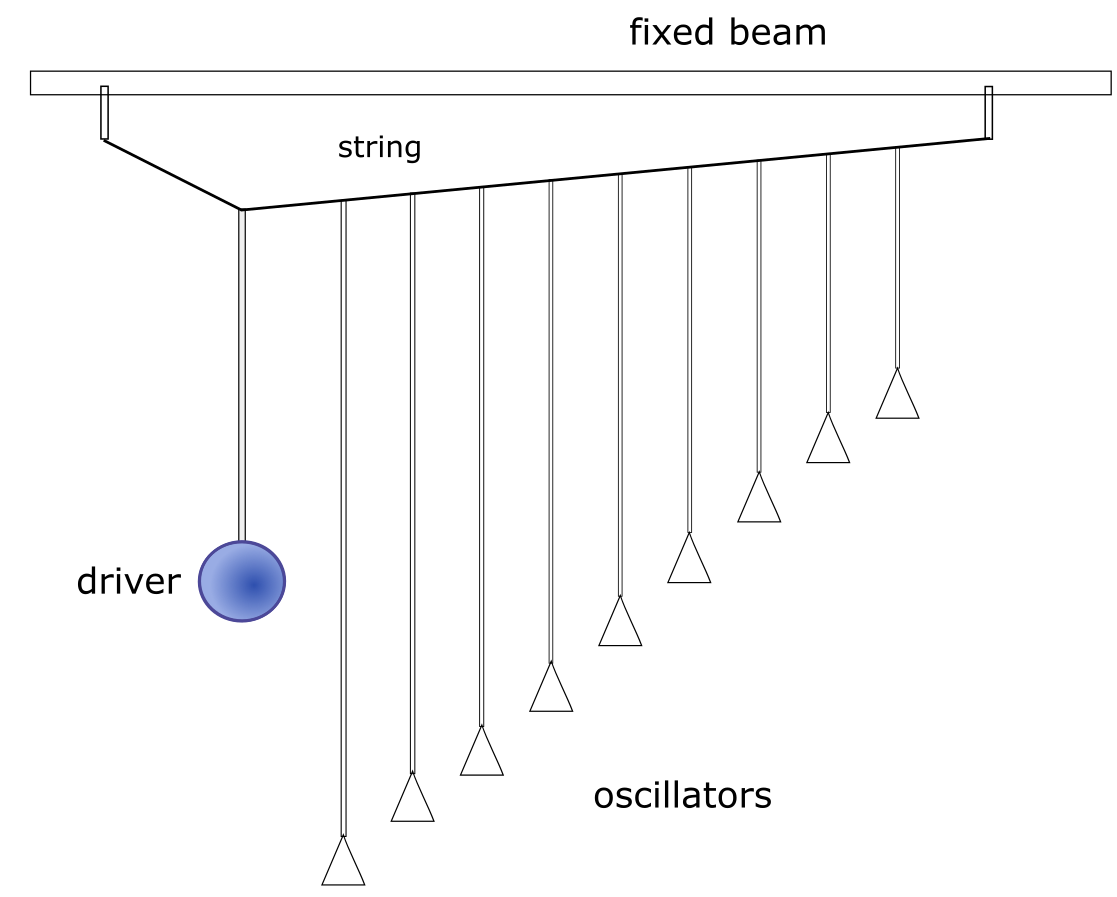
\includegraphics[width = 0.6\textwidth]{figures/chapter04/bartons_pendulums.png}
    \vspace{-15pt}
    \caption{A diagram of the Barton's pendulums experiment (courtesy Wikipedia).}
    \vspace{-10pt}
    \label{fig:bartons_pendulums}
\end{figure}

Resonant absorption is essential in the field of coronal seismology. Coronal seismology is a technique which enables solar physicists to infer coronal quantities (e.g. plasma density or magnetic field strength) by studying observed MHD waves. The technique usually involves recording data that can be measured relatively easily, e.g. wave period, wavelength, amplitude, damping time and then using MHD wave theory to infer harder to measure quantities like the magnetic field strength or density gradient. Resonant absorption can play a key role in damping observed coronal loop oscillations \citep{Nakariakov1999, Terradas2006}. \citet{Ruderman2002} shows that a kink wave in a cylindrical wave can mode convert to a torsional Alfv\'en wave. This results in the amplitude of the kink wave following a decay profile closely resembling that of observed decay profiles. Also, resonant absorption leads to the development of short length scales through phase mixing, leading to heating. \citet{Poedts1989,Ofman1995} suggest that resonant absorption could explain coronal heating. However, \citet{Prokopyszyn2019b} argue that the heating rate is too slow for observed wave amplitudes and frequencies.

This chapter focuses on studying resonant absorption when the background magnetic field is oblique to the boundary. In \citet{Halberstadt1993,Halberstadt1995} they modelled resonant absorption in the corona and showed that tilting the background magnetic field and imposing line-tied boundary conditions causes the formation of evanescent fast wave boundary layers. These boundary layers have also been studied numerically in \citet{Arregui2003}. Since the evanescent fast waves form at the boundary, we believe it is worth checking the validity of the boundary conditions. To test the validity, we check if a model where the chromosphere is included instead of imposing line-tied boundary conditions can still produce the same evanescent fast waves. We believe we are the first authors to study the boundary layers in a model where the chromosphere and corona are included. The corona and chromosphere are modelled using a piecewise constant background density profile with a discontinuous jump from the corona to the chromosphere.

Previous chapters injected waves using a footpoint driver, whereas, this chapter drives from the side for mathematical convenience.
These waves could be generated by, for example, a nearby flare. However, it is not our aim to investigate how the waves enter the corona, but instead, we study their dynamics once they are in the corona. The origin of coronal waves remains an open question. It is difficult for Alfvén waves generated at the photosphere to enter the corona \citep{Cranmer2005}, due to the rapid exponential decay of the density with height in the chromosphere and the steep decrease at the transition region. \citet{Hollweg1984b} suggests resonances in coronal loops and spicules provide enough energy flux to the corona to match the observed wave velocity amplitudes. \citet{Cally2011,Hansen2012} suggest that mode conversion from fast waves to Alfv\'en waves at the transition region enables sufficient energy flux to enter the corona. It is also possible that the corona itself generates Alfvén waves via magnetic reconnection \citep{Cranmer2018} and the energy released during reconnection partially feeds into the energy contained in the Alfv\'en waves.
% Instead of studying how waves enter the corona, we study their dynamics after entering the corona. How waves are generated in the corona remains an open question. The exponential density and the steep jump in density at the transition region make it difficult for Alfv\'en waves generated at the photosphere to enter the corona \citep{Cranmer2005}. \citet{Hollweg1984b} suggests resonances in coronal loops and spicules provide enough energy flux to the corona. \citet{Cally2011,Hansen2012} suggest that mode conversion from fast waves to Alfv\'en waves at the transition region enables sufficient energy flux to enter the corona. It is also possible that the corona itself generates Alfv\'en waves via magnetic reconnection \citep{Cranmer2018}.

This chapters outline is as follows; in Sections \ref{sec:chap_4_model_and_eqns} and \ref{sec:chap_4_energy_equations} we  present the equations we will use to model the plasma and then discuss the applicability of some of the assumptions we make in the corona. Section \ref{sec:normal_field_resonant_absorption_with_line_tied_bcs} introduces some of the key and most relevant properties of resonant absorption in a simple domain where the background magnetic field is perpendicular to the $z=z_{min}$ and $z=z_{max}$ boundaries. In Section \ref{sec:oblique_field_uniform_density_profile_with_line_tied_bcs}, we calculate normal mode solutions in a domain where the Alfv\'en speed is uniform. We impose an incident Alfv\'en wave and calculate the unique solution which ensures the velocity is zero at $z=0$. Since the Alfv\'en speed is uniform, resonant absorption cannot occur. However, we choose the length scales in $x$ to be extremely short to simulate the conditions near a singularity in a resonant absorption experiment. Section \ref{sec:oblique_field_piecewise_constant_density_profile} builds on Section \ref{sec:oblique_field_uniform_density_profile_with_line_tied_bcs} by using a background Alf\'en speed which is piecewise constant in $z$. The regions $z>0$ and $z<0$ corresponds to the corona and chromosphere, respectively. We impose an incident Alfv\'en wave and calculate the unique solution which ensures continuity of the velocity and its derivative at $z=0$. By comparing results from Sections \ref{sec:oblique_field_uniform_density_profile_with_line_tied_bcs} and \ref{sec:oblique_field_piecewise_constant_density_profile}, we can test how robust the boundary layers produced by line-tied boundary conditions are when we consider the finite nature of the jump in Alfv\'en speeds and the small length scales of a resonance layer. In Section \ref{sec:oblique_field_resonant_absorption} we use a background Alfv\'en speed which is a function of $x$ and piecewise constant in $z$. Our goal here is to test if steep boundary layers form in a resonant absorption experiment. Finally, in Section \ref{sec:chap_4_conclusions}, a summary of our results and conclusions are given.

% In this chapter, we start by giving an overview of the model and the equations we will use in Sections \ref{sec:chap_4_model_and_eqns} and \ref{sec:chap_4_energy_equations}. Section \ref{sec:normal_field_resonant_absorption_with_line_tied_bcs} introduces some of the key and most relevant properties of resonant absorption in a simple domain where the background magnetic field is perpendicular to the $z=z_{min}$ and $z=z_{max}$ boundaries. In Section \ref{sec:oblique_field_uniform_density_profile_with_line_tied_bcs} we model the background magnetic field as oblique to the boundaries and we calculate normal mode solutions in a domain where the Alfv\'en speed is uniform. We impose an incident Alfv\'en wave and calculate the unique solution which ensures the velocity is zero at $z=0$. Since the Alfv\'en speed is uniform, resonant absorption cannot occur. However, we choose very short length scales in $x$ to simulate the conditions near a singularity in a resonant absorption experiment. Section \ref{sec:oblique_field_piecewise_constant_density_profile} builds on Section \ref{sec:oblique_field_uniform_density_profile_with_line_tied_bcs} by using a piecewise constant in $z$ background Alf\'en speed. The regions $z>0$ and $z<0$ corresponds to the corona and chromosphere respectively. We impose an incident Alfv\'en wave and calculate the unique solution which ensures continuity of the velocity and its derivative at $z=0$. By comparing results from Sections \ref{sec:oblique_field_uniform_density_profile_with_line_tied_bcs} and \ref{sec:oblique_field_piecewise_constant_density_profile} we can test if the boundary layers produced by line-tied boundary conditions are physical. In Section \ref{sec:oblique_field_resonant_absorption} we use a background Alfv\'en speed which is a function of $x$ and piecewise constant in $z$. Our goal here is to test if steep boundary layers form in a resonant absorption experiment. Finally, in Section \ref{sec:chap_4_conclusions} a summary of our results and conclusions are given.

% we consider the case where the magnetic field to be oblique to the boundary. Section \ref{sec:oblique_field_piecewise_constant_density_profile} builds on Section  we consider the case where the Alfv\'en speed is uniform in $x$ as our goal is to understand why the boundary layers form at the transition region in as simple a domain as possible. Section \ref{sec:oblique_field_resonant_absorption} builds on Section \ref{sec:oblique_field_piecewise_constant_density_profile} by modelling the case where the Alfv\'en speed is a function of $x$ as this is necessary for resonant absorption to occur. Finally in Section \ref{sec:oblique_field_uniform_density_profile_with_line_tied_bcs} we consider the case where line-tied boundary conditions are used to test if the magnitude of the boundary layers which are formed when line-tied boundary conditions are used is physical and approximately agrees with the solution when the chromosphere is included in the model.

\section{Model and equations}
\label{sec:chap_4_model_and_eqns}

In this section, we describe the most general model we will use. However, throughout this paper, we will start with a simple model. In subsequent sections, we will add complexity to the model as we head
towards the most relevant description of resonance in coronal magnetic fields. For example, in Sections \ref{sec:oblique_field_uniform_density_profile_with_line_tied_bcs} and \ref{sec:oblique_field_piecewise_constant_density_profile}, the background Alfv\'en speed, $v_A$, will not depend on $x$ but, in Section \ref{sec:oblique_field_resonant_absorption}, we include a variation in $x$ as well as a model chromosphere. 

We model perturbations on a static background equilibrium and make the same assumptions as those described by Equation \eqref{eq:linear_assumotion_v}-\eqref{eq:linear_assumotion_rho}. The system is assumed to be ideal, i.e. we neglect viscosity and resistivity. We model the plasma as cold, i.e. $\beta=0$, which means the magnetic pressure force is negligible. We assume the Lorentz force dominates and neglect the gravitational force. The background magnetic field is at an angle $\alpha$ to the $z$-axis in the $y$-$z$ plane, i.e.
\begin{equation}
    \label{eq:chap_4_background_field}
    \begin{aligned}
    \vec{B}_0 &= B_0(\sin\alpha\,\vec{\hat{y}}+\cos\alpha\,\vec{\hat{z}}) \\
    &= B_0\vec{\hat{B}}_0,
    \end{aligned}
\end{equation}
The unit vectors, $\vec{\hat{B}}_0$ and $\vec{\hat{\perp}}$, are defined as
\begin{gather}
    \vec{\hat{B}}_0 = \sin\alpha\,\vec{\hat{y}}+\cos\alpha\,\vec{\hat{z}}, \\
    \vec{\hat{\perp}} = \cos\alpha\,\vec{\hat{y}}-\sin\alpha\,\vec{\hat{z}},
\end{gather}
where both unit vectors are in the $y$-$z$ plane, $\vec{\hat{B}}_0$ is parallel to the background magnetic field and $\vec{\hat{\perp}}$ is perpendicular to the background magnetic field. 
The background Alfv\'en speed is given by $v_A(x,z) = \hat{v}_A(x)v_{A}(0,z)$, where
\begin{equation}
    \label{eq:chap_4_vA(0,z)}
    v_A(0,z)= \begin{cases}
    v_{A-}, & z < 0, \\
    v_{A+}, & z \ge 0,
    \end{cases}
\end{equation}
and $\hat{v}_A(x)$ is an arbitrary function of $x$ satisfying $\hat{v}_A(0)=1$. The region $z<0$ models the chromosphere and the region $z>0$ models the corona, therefore, $v_{A+}>v_{A-}$ due to the higher density in the chromosphere.

The variables we solve for are the velocity, $\vec{u}$, given by
\begin{equation}
    \vec{u}(x,y,z) = u_x\vec{\hat{x}} + u_\perp \vec{\hat{\perp}}
\end{equation}
and the magnetic field perturbations, $\vec{b}$, given by
\begin{equation}
    \vec{b}(x,y,z) = b_x\vec{\hat{x}} + b_\perp \vec{\hat{\perp}} + b_{||}\vec{\hat{B}}_0,
\end{equation}
where
\begin{equation}
\begin{aligned}
    \vec{\hat{b}}(x,y,z) &= \hat{b}_x\vec{\hat{x}} + \hat{b}_\perp \vec{\hat{\perp}} + \hat{b}_{||}\vec{\hat{B}}_0 \\
    &= \frac{\vec{b}}{B_0}.
\end{aligned}
\end{equation}

The linearised momentum equation simplifies to
\begin{equation}
    \label{eq:chap_4_linearised_momentum_eqn}
    \begin{aligned}
        \pdv{\vec{u}}{t}=\frac{1}{\mu\rho(x,z)}\qty[(\vec{B}_0\cdot\grad)\vec{b} - \grad\qty(\vec{b}\cdot\vec{B}_0)],
    \end{aligned}
\end{equation}
and the induction equation simplifies to
\begin{equation}
    \label{eq:chap_4_linearised_induction_eqn}
    \begin{aligned}
    \pdv{\vec{b}}{t}=(\vec{B}_0\cdot\grad)\vec{u} - \vec{B}_0\div{\vec{u}}.
    \end{aligned}
\end{equation}
Written out component-wise the above equations become
\begin{gather}
    \label{eq:chap_4_ux_eqn1}
    \pdv{u_x}{t}=v_A^2(x,z)\left[\nabla_{||}\hat{b}_x - \pdv{\hat{b}_{||}}{x}\right],\\
    \label{eq:chap_4_u_perp_eqn1}
    \pdv{u_\perp}{t}=v_A^2(x,z)\left[\nabla_{||}\hat{b}_\perp-\nabla_\perp \hat{b}_{||}\right],\\
    \label{eq:chap_4_bx_eqn1}
    \pdv{\hat{b}_x}{t}=\nabla_{||}u_x,\\
    \label{eq:chap_4_b_perp_eqn1}
    \pdv{\hat{b}_\perp}{t}=\nabla_{||}u_{\perp},\\
    \label{eq:chap_4_b_par_eqn1}
    \pdv{\hat{b}_{||}}{t}=-\left[\pdv{u_x}{x}+\nabla_\perp u_{\perp}\right],
\end{gather}
where
\begin{gather}
    \label{eq:nabla_perp}
    \begin{aligned}
    \nabla_\perp &= \vec{\hat{\perp}}\vdot\grad \\
    &= \cos\alpha\pdv{}{y}-\sin\alpha\pdv{}{z},
    \end{aligned} \\
    \label{eq:nabla_par}
    \begin{aligned}
    \nabla_{||} &= \vec{\hat{B}}_0\vdot\grad \\
    &= \sin\alpha\pdv{}{y}+\cos\alpha\pdv{}{z},
    \end{aligned}
\end{gather}
are the derivatives perpendicular and parallel to the
equilibrium magnetic field respectively.

In this chapter, we will derive exact analytic solutions to the equations. However, the formulas we derive are often cumbersome, and so our discussion will often focus on approximate (but less cumbersome) solutions in our narrower parameter space. The parameter space we will focus on is
\begin{gather}
    \label{eq:parm_space_1}
    k_x \gg k_{||+}, \\
     \label{eq:parm_space_2}
    k_{||-} \gg k_{||+}, \\
    \label{eq:parm_space_ky}
    0 < k_y \le O(k_{||+}), \\
    \label{eq:parm_space_4}
    0 < \tan\alpha \le O(1), 
\end{gather}
where 
\begin{gather}
    \label{eq:k_par_pm}
    k_{||\pm} = \frac{\omega}{v_{A\pm}}, \\
    \label{eq:k_par0}
    k_{||0} = \frac{\omega}{v_{A0}}
\end{gather}
gives the Alfv\'en wavenumber and $\omega$ gives the wave frequency. We model $k_x\gg k_{||+}$ as this approximates the conditions near a singularity in a resonant absorption experiment. The results should also apply to other cases where $k_x\gg k_{||+}$, for example, during the nonlinear development of an instability. Our condition for $\alpha$ prevents the background magnetic field from being tangential to the $z=0$ plane.


\section{Energy equations}
\label{sec:chap_4_energy_equations}

Resonant absorption occurs due to fast waves mode converting into Alfv\'en waves at a resonant field line. This can be better understood by considering how the oscillations in the $x$ and $\vec{\hat{B}}_0$ direction couple to the fluctuations in the $\perp$-direction. Note that the $x$ and $||$ perturbation energy density is given by
\[\frac{1}{2}\rho u_x^2 + \frac{b_x^2}{2\mu} + \frac{b_{||}^2}{2\mu},\]
and the $\perp$-energy density is given by
\[\frac{1}{2}\rho u_\perp^2 + \frac{b_\perp^2}{2\mu} .\]

Taking the dot product of Equation \eqref{eq:chap_4_linearised_momentum_eqn} with $\vec{u}_x=u_x\vec{\hat{x}}$ gives
\[\pdv{}{t}\left(\frac{1}{2}\rho u_x^2\right)=\frac{1}{\mu}[(\vec{B}_0\cdot\vec{\nabla})b_x]u_x-\frac{B_0}{\mu}\pdv{b_{||}}{x}u_x.\]
Taking the dot product of Equation \eqref{eq:chap_4_linearised_momentum_eqn} with $\vec{b}_x=b_x\vec{\hat{x}}$ gives
\[\pdv{}{t}\left(\frac{b_x^2}{2\mu}\right)=\frac{1}{\mu}[(\vec{B}_0\cdot\vec{\nabla})u_x]b_x.\]
Note that,
\[\vec{\nabla}\cdot\left(\frac{\vec{E}\times\vec{b}_x}{\mu}\right)=-\frac{1}{\mu}\vec{B}_0\cdot\vec{\nabla}(u_xb_x),\]
hence,
\begin{equation}
    \label{eq:chap_4_x_energy}
    \pdv{}{t}\left(\frac{1}{2}\rho u_x^2+\frac{b_x^2}{2\mu}\right)+\vec{\nabla}\cdot\left(\frac{\vec{E}\times\vec{b}_x}{\mu}\right)=-\frac{B_0}{\mu}u_x\pdv{b_{||}}{x}.
\end{equation}
Similarly, we can show that
\begin{gather}
    \label{eq:chap_4_perp_energy}
    \pdv{}{t}\left(\frac{1}{2}\rho u_\perp^2+\frac{b_\perp^2}{2\mu}\right)+\vec{\nabla}\cdot\left(\frac{\vec{E}\times\vec{b}_\perp}{\mu}\right)=-\frac{B_0}{\mu}u_\perp\nabla_\perp b_{||}, \\
    \label{eq:chap_4_par_energy}
    \pdv{}{t}\left(\frac{b_{||}^2}{2\mu}\right)+\vec{\nabla}\cdot\left(\frac{\vec{E}\times\vec{b}_{||}}{\mu}\right)=\frac{B_0}{\mu}(\vec{u}\cdot\vec{\nabla})b_{||}.
\end{gather}
Adding Equation \eqref{eq:chap_4_x_energy} to \eqref{eq:chap_4_par_energy} gives
\begin{equation}
    \label{eq:chap_4_fast_energy}
    \pdv{}{t}\left(\frac{1}{2}\rho u_x^2+\frac{b_x^2+b_{||}^2}{2\mu}\right)+\vec{\nabla}\cdot\left[\frac{\vec{E}\times(\vec{b}_x+\vec{b}_{||})}{\mu}\right]=\frac{B_0}{\mu}u_\perp\nabla_\perp b_{||}.
\end{equation}
% In this chapter, we can think of Equations \eqref{eq:chap_4_fast_energy} and as describing the evolution of the fast wave energy and Alfv\'en wave energies respectively because we will show in for example.
Equations \eqref{eq:chap_4_perp_energy} and \eqref{eq:chap_4_fast_energy} show that gradients in the magnetic pressure, $B_0b_{||}/\mu$, are responsible for the mode conversion from oscillations in the $x$, $||$ directions to oscillations in the $\perp$ direction. If $\nabla_\perp = 0$ then no mode conversion can occur between the fast and Alfv\'en waves and they are independent of one another.

\section{Normal field: Resonant absorption with line-tied BCs}
\label{sec:normal_field_resonant_absorption_with_line_tied_bcs}

This section aims to introduce resonant absorption by calculating the solution for the simple case where $\alpha=0$. Therefore, the background magnetic field points in the $z$-direction. We aim to show how the waves can form very short length-scales if the system has a relatively small gradient in Alfv\'en travel time across the background magnetic field lines.

\subsection{Equations}

For simplicity, we will model the chromosphere as infinitely denser than the corona, i.e. $v_{A-}\rightarrow 0$. We will model the $z$-range as $0\le z\le L_z$ and impose line-tied boundary conditions at $z=0$ and $z=L_z$, i.e. 
\begin{equation}
    u_x|_{z=0}=u_x|_{z=L_z}=u_y|_{z=0}=u_y|_{z=L_z}=0.
\end{equation}
Therefore, $v_A=v_A(x)$. The $x$ domain is given by $x\ge x_{min}$ and we impose a driver at $x=x_{min}$, of the form
\begin{gather}
    \label{eq:chap_4_x_min_bcs_alpha=0}
    u_x(x_{min},y,z,t) = f_{driv}(y,z,t), \\
    \left.\pdv{u_x}{x}\right|_{x=x_{min}} = g_{driv}(y,z,t).
\end{gather}

Since $\alpha=0$, this means that $u_y = u_\perp$, $b_y = b_{\perp}$ and $b_z = b_{||}$. Also, $\nabla_\perp=\pdv*{}{y}$ and $\nabla_{||}=\pdv*{}{z}$. Therefore, Equations \eqref{eq:chap_4_ux_eqn1}-\eqref{eq:chap_4_b_par_eqn1} can be written as
\begin{gather}
    \label{eq:chap_4_ux_eqn_alpha=0}
    \pdv{u_x}{t} = v_A^2(x)\qty[\pdv{\hat{b}_x}{z} - \pdv{\hat{b}_z}{x}],\\
    \pdv{u_y}{t} = v_A^2(x)\qty[\pdv{\hat{b}_y}{z} - \pdv{\hat{b}_z}{y}],\\
    \pdv{\hat{b}_x}{t} = \pdv{u_x}{z},\\
    \pdv{\hat{b}_y}{t} = \pdv{u_y}{z},\\
    \label{eq:chap_4_bz_eqn_alpha=0}
    \pdv{\hat{b}_z}{t} = -\qty[\pdv{u_x}{x} + \pdv{u_y}{y}].
\end{gather}

\subsection{Analytic solution}
\label{sec:chap_4_normal_mode_analytic_solution}

The problem is linear and the functions we need to solve for depend on just $x$. Therefore, by assuming a Fourier solution in $y$, $z$ and $t$ we can convert the PDEs, \eqref{eq:chap_4_ux_eqn_alpha=0}-\eqref{eq:chap_4_bz_eqn_alpha=0} into a set of ODEs.
We assume the solutions are of the form
\begin{gather}
    \label{eq:chap_4_ux_expansion}
    u_x(x,y,z,t) = \sum_{n=1}^\infty u_{xn}(x)\sin(k_{zn}z)\exp[i(k_y y + \omega t)], \\
    u_y(x,y,z,t) = \sum_{n=1}^\infty u_{yn}(x)\sin(k_{zn}z)\exp[i(k_y y + \omega t)], \\
    \hat{b}_x(x,y,z,t) = \sum_{n=1}^\infty \hat{b}_{xn}(x)\sin(k_{zn}z)\exp[i(k_y y + \omega t)], \\
    \hat{b}_y(x,y,z,t) = \sum_{n=1}^\infty \hat{b}_{yn}(x)\sin(k_{zn}z)\exp[i(k_y y + \omega t)], \\
    \label{eq:chap_4_bz_expansion}
    \hat{b}_z(x,y,z,t) = \sum_{n=1}^\infty \hat{b}_{zn}(x)\sin(k_{zn}z)\exp[i(k_y y + \omega t)],
\end{gather}
where $k_y$, $\omega$ are constants,
\begin{equation}
    k_{zn} = \frac{n\pi}{L_z},
\end{equation}
this ensures the line-tied boundary conditions in $z$ are automatically satisfied. Substituting the above series into Equations \eqref{eq:chap_4_ux_eqn_alpha=0}-\eqref{eq:chap_4_bz_eqn_alpha=0}, and multiplying by $\sin(k_{zm}z)$ and integrating from $0$ to $L_z$ gives.
\begin{gather}
    i\omega u_{xm} = v_A^2(x)\qty[ik_{zm} \hat{b}_{xm} - \dv{\hat{b}_{zm}}{x}],\\
    i\omega u_{ym} = v_A^2(x)\qty[ik_{zm} \hat{b}_{xm} - ik_y \hat{b}_{zm}],\\
    i\omega \hat{b}_{xm} = ik_{zm}u_{xm},\\
    i\omega \hat{b}_{ym} = ik_{zm}u_{ym},\\
    \label{eq:chap_4_bz_eqn2_alpha=0}
    i\omega \hat{b}_{zm} = -\qty[\dv{u_{xm}}{x}+ ik_yu_{ym}].
\end{gather}
Let
\begin{equation}
    \mathcal{L}_n(x) = \frac{\omega^2}{v_A^2(x)} - k_{zn}^2.
\end{equation}
Eliminating $\hat{b}_{xn}$ and $\hat{b}_{yn}$ gives
\begin{gather}
   \mathcal{L}_n(x)u_{xn}(x)=i\omega \dv{\hat{b}_{zn}}{x}, \\
   \label{eq:chap_4_uy_eqn_bz}
   \mathcal{L}_n(x)u_{yn}(x)=ik_y i\omega \hat{b}_{zn}.
\end{gather}
Eliminating $\hat{b}_{zn}$ gives
\begin{gather}
    \label{eq:chap_4_ux_eqn2_alpha=0}
    \dv[2]{u_{xn}}{x}+\mathcal{L}_n(x)u_{xn}(x)=-ik_y\dv{u_{yn}}{x},\\
    \label{eq:chap_4_uy_eqn2_alpha=0}
    \qty[\mathcal{L}_n(x)-k_y^2]u_{yn}(x)=-ik_y\dv{u_{xn}}{x}.
\end{gather}
Eliminating $u_{yn}$ from Equation \eqref{eq:chap_4_ux_eqn2_alpha=0}, using Equation \eqref{eq:chap_4_uy_eqn2_alpha=0}, gives
\[
    \begin{aligned}
    \dv[2]{u_{xn}}{x}+\mathcal{L}_n(x)u_{xn}(x)&=-ik_y\dv{}{x}\qty[\frac{-ik_y}{\mathcal{L}_n(x)-k_y^2}\dv{u_{xn}}{x}] \\
    &=\frac{-k_y^2}{\mathcal{L}_n(x)-k_y^2}\qty[\dv[2]{u_{xn}}{x}-\frac{\mathcal{L}_x(x)}{\mathcal{L}_n(x)-k_y^2}\dv{u_{xn}}{x}],
    \end{aligned}
\]
where
\begin{gather}
\begin{aligned}
    \mathcal{L}_x(x) &= \dv{\mathcal{L}_n}{x} \\
    &= -2\frac{\omega^2}{v_A^3(x)}\dv{v_A}{x} \\
    &= -\frac{2\omega^2}{v_A^2(x)a(x)},
\end{aligned} \\
    \tag{\ref{eq:length_scale_alfven_travel_time}}
    a(x) = \frac{v_A(x)}{\dv*{v_A}{x}}.
\end{gather}
Rearranging gives
\begin{equation}
    \label{eq:uxn_ode1}
    \mathcal{L}_n(x)\dv[2]{u_{xn}}{x}-\frac{k_y^2\mathcal{L}_x(x)}{\mathcal{L}_n(x)-k_y^2}\dv{u_{xn}}{x}+\mathcal{L}_n(x)[\mathcal{L}_n(x)-k_y^2]u_{xn}(x)=0.
\end{equation}

We can eliminate $u_x$ to get an equation for $u_\perp$ via the following procedure. Take the $x$-derivative of Equation \eqref{eq:chap_4_ux_eqn2_alpha=0} to give
\[
    u_{xn}(x) = -\frac{1}{\mathcal{L}_n'(x)}\qty{\qty[\dv[2]{}{x}+\mathcal{L}_n]\dv{u_{xn}}{x}+ik_y\dv[2]{u_{yn}}{x}}.
\]
Substitute this into Equation \eqref{eq:chap_4_ux_eqn2_alpha=0} to give
\[
    \dv[2]{u_{xn}}{x}-\frac{\mathcal{L}_n}{\mathcal{L}_x}\qty{\qty[\dv[2]{}{x}+\mathcal{L}_n]\dv{u_{xn}}{x}+ik_y\dv[2]{u_{yn}}{x}}=-ik_y\dv{u_{yn}}{x},
\]
where we have assumed $\mathcal{L}_x(x)\ne0$. See for example \citet{Thompson1993} for a calculation of the solution in the case where $\mathcal{L}_n(x)=\mathcal{L}_x(x)=0$.
Multiply through by $-ik_y$ and eliminate $u_{xn}$ using Equation \eqref{eq:chap_4_uy_eqn2_alpha=0} to give
\[
\begin{aligned}
    &\dv{}{x}[(\mathcal{L}_n-k_y^2)u_{yn}]-\\
    &\frac{\mathcal{L}_n}{\mathcal{L}_x(x)}\qty{\qty[\dv[2]{}{x}+\mathcal{L}_n]\qty[\mathcal{L}_n-k_y^2]u_{yn}+k_y^2\dv[2]{u_{yn}}{x}}=-k_y^2\dv{u_{yn}}{x}.
\end{aligned}
\]
This can be simplified to give
\begin{equation}
\label{eq:chap_4_uy_ode}
    \mathcal{L}_n^2\dv[2]{u_{yn}}{x}+\mathcal{L}_x\mathcal{L}_n\dv{u_{yn}}{x}+(\mathcal{L}_n^3+\mathcal{L}_{xx}\mathcal{L}_n-k_y^2\mathcal{L}_n-\mathcal{L}_x^2) u_{yn}=0,
\end{equation}
where
\begin{equation}
    % \mathcal{M}_n = \mathcal{L}_n^3+\mathcal{L}_{xx}\mathcal{L}_n-k_y^2\mathcal{L}_n-\mathcal{L}_x^2, \\
    \mathcal{L}_{xx} = \dv{\mathcal{L}_x}{x}.
\end{equation}

Our goal now is to solve Equations \eqref{eq:uxn_ode1} and \eqref{eq:chap_4_uy_ode} using the method of Frobenius. Assume that $\mathcal{L}_n$ is an analytic function. Therefore, points where $\mathcal{L}_n(x)\ne0$ are ordinary/regular points of Equation \eqref{eq:chap_4_uy_ode} and points where $\mathcal{L}_n(x)=0$ are regular-singular points of the ODE. Let $x_{res,n}$ be defined as a point satisfying $\mathcal{L}_n(x_{res,n})=0$. If multiple points satisfy $\mathcal{L}_n(x)=0$, then pick $x_{res,n}$ equal to one of these points arbitrarily. Since we expect solutions $u_{yn}$ to be singular at $x=x_{res,n}$, we will focus on studying solutions near this point.

\subsubsection{Radius of convergence}

Multiplying Equation \eqref{eq:uxn_ode1} through by $(x-x_{res,n})^2/\mathcal{L}_n(x)$ gives
\begin{equation}
    \label{eq:uxn_ode2}
    (x-x_{res,n})^2\dv[2]{u_{xn}}{x} + (x-x_{res,n})p_n(x)\dv{u_{xn}}{x} + q_n(x)u_{xn}(x)=0,
\end{equation}
where
\begin{gather}
    p_n(x) = -\frac{k_y^2\mathcal{L}_x(x)(x-x_{res,n})}{\mathcal{L}_n(x)(\mathcal{L}_n(x)-k_y^2)}, \\
    q_n(x) = (\mathcal{L}_n(x)-k_y^2)(x-x_{res,n})^2.
\end{gather}
The power series solution for $u_{xn}$ about $x=x_{res,n}$ will have a radius of convergence at least as large as the radius of convergence for the power series of $p_n(x)$ and $q_n(x)$ about $x=x_{res,n}$. Since $\mathcal{L}_n(x)$ is analytic we expect the radius of convergence for $q_n$ to be infinite. The radius of convergence of $p_n(x)$ (denoted with $R_n$) is equal to the distance in the complex plane between $x_{res,n}$ and the nearest zero of $\mathcal{L}_n(x)(\mathcal{L}_n(x)-k_y^2)$ (excluding the point $x=x_{res,n}$). Hence, the radius of convergence for $u_{xn}$ about $x=x_{res,n}$ is at least as large as $R_n$.

\subsubsection{Indicial polynomial}

To calculate the solution via the method of Frobenius we first need to calculate the indicial polynomial. Substituting
\[u_{xn}(x)=(x-x_{res,n})^\sigma\sum_{k=0}^\infty a_k(x-x_{res,n})^k,\]
into Equation \eqref{eq:uxn_ode2} gives
\[\sum_{k=0}^\infty [(k + \sigma - 1)(k+\sigma) + (k+\sigma)p_n(x) + q_n(x)]a_k(x-x_{res,n})^k=0.\]
We need to find values of $\sigma$ where non-trivial solutions can exist.
Taylor expanding $p(x)$ and $q(x)$ about $x=x_{res,n}$, we calculate the coefficient of the leading order power in $(x-x_{res,n})$ to be given by
\begin{equation}
    I(\sigma) = (\sigma-1)\sigma + p_n(x_{res,n})\sigma + q_n(x_{res,n}),
\end{equation}
where $I(\sigma)$ is the indicial polynomial. Since $I(\sigma)=0$, $p_n(x_{res,n})=1$ and $q_n(x_{res,n})=0$ we know that $\sigma^2=0$. Since we have repeated roots the general solution  is given by a linear combination of
\begin{equation}
    u_{xn1}(x) = \sum_{k=0}^\infty a_k(x-x_{res,n})^k,
\end{equation}
and
\begin{equation}
    u_{xn2}(x) = u_{xn1}(x)\ln(x-x_{res,n}) + \sum_{k=1}^\infty b_k(x-x_{res,n})^k.
\end{equation}

\subsubsection{Recurrence relations}

We will now calculate the recurrence relation for the $a_k$ terms. Substituting $u_{xn1}(x)$ into Equation \eqref{eq:uxn_ode2} and Taylor expanding $p_n(x)$ and $q_n(x)$ about $x=x_{res,n}$ gives
\[\sum_{k=0}^\infty\qty[I(k)a_k+\sum_{j=0}^{k-1}\frac{jp_n^{(k-j)}(x_{res,n})+q_n^{(k-j)}(x_{res,n})}{(k-j)!}a_j] \qty(x-x_{res,n})^k=0.\]
Equating the coefficient of $(x-x_{res,n})^k$ equal to zero gives the following recurrence relation,
\begin{equation}
    a_k = -\frac{1}{I(k)}\sum_{j=0}^{k-1}\frac{jp_n^{(k-j)}(x_{res,n})+q_n^{(k-j)}(x_{res,n})}{(k-j)!}a_j,
\end{equation}
for $k\ge1$, where we arbitrarily set $a_0=1$. Setting $a_0=1$ does not lose generality as $u_{xn}$ is equal to a linear combination of $u_{xn1}$ and $u_{xn2}$. Since $q_n'(x_{res,n})=0$ we know that $a_1=0$.

We will now calculate an expression for the $b_k$ terms. Note that
\[\dv{u_{xn2}}{x} = \dv{u_{xn1}}{x}\ln(x-x_{res,n}) + \frac{u_{xn1}}{x-x_{res,n}} + \sum_{k=1}^\infty kb_k(x-x_{res,n})^{k-1},\]
\[\begin{aligned}
\dv[2]{u_{xn2}}{x} &= \dv[2]{u_{xn1}}{x}\ln(x-x_{res,n}) + \frac{2}{x-x_{res,n}}\dv{u_{xn1}}{x} - \frac{u_{xn1}}{(x-x_{res,n})^2} \\
&+ \sum_{k=1}^\infty k(k-1)b_k(x-x_{res,n})^{k-2}.
\end{aligned}\]
Hence, substituting $u_{xn2}(x)$ into Equation \eqref{eq:uxn_ode2} gives
\[\begin{aligned}
&2(x-x_{res,n})\dv{u_{xn1}}{x}+[p_n(x) - 1]u_{xn1}(x) + \\
&\qquad\sum_{k=1}^\infty[k(k - 1) + kp_n(x) + q_n(x)]b_k(x-x_{res,n})^k = 0.
\end{aligned}\]
Substituting for $u_{xn1}(x)$ gives
\[\begin{aligned}
&\sum_{k=0}^\infty[2k + p_n(x) - 1]a_k(x-x_{res,n})^k + \\
&\qquad\sum_{k=1}^\infty [k(k - 1) + kp_n(x) + q_n(x)]b_k(x-x_{res,n})^k = 0.
\end{aligned}\]
Taylor expanding $p_n(x)$, $q_n(x)$ about $x=x_{res,n}$ gives
\[\begin{aligned}
&\sum_{k=0}^\infty\qty[(2k + p_n(0) - 1)a_k + \sum_{j=0}^{k-1}\frac{p_n^{(k-j)}(x_{res,n})}{(k-j)!}a_j] \qty(x-x_{res,n})^k + \\
&\qquad\sum_{k=1}^\infty \qty[I(k)b_k + \sum_{j=1}^{k-1}\frac{jp_n^{(k-j)}(x_{res,n})+q_n^{(k-j)}(x_{res,n})}{(k-j)!}b_j] \qty(x-x_{res,n})^k = 0.
\end{aligned}\]
Equating the coefficient of $(x-x_{res,n})^k$ equal to zero gives
% \begin{equation}
%     \begin{aligned}
%     a_0 &= \frac{p_n'(x_{res,n})-q_n'(x_{res,n})}{I(0)}a_{-1} \\
%         &= \frac{4\mathcal{L}_{xx}(x_{res,n}) - k_y^2}{\mathcal{L}_x(x_{res,n})}a_{-1}
%     \end{aligned}
% \end{equation}
% where,
% Equating the coefficient of $(x-x_{res,n})^1$ equal to zero gives
% \[2Ca_1+\sum_{j=-1}^0\frac{jp_n^{(1-j)}(x_{res,n})+q_n^{(1-j)}(x_{res,n})}{(1-j)!}b_j=0,\]
% hence, $C$ is given by
% \begin{equation}
%     C=-\frac{1}{2a_1}\sum_{j=-1}^0\frac{jp_n^{(1-j)}(x_{res,n})+q_n^{(1-j)}(x_{res,n})}{(1-j)!}b_j=0,
% \end{equation}
% for $a_1\ne0$. If $a_1=0$ then $C$ can be arbitrary. Equating the coefficient of $(x-x_{res,n})^k$ for $k\ge1$ gives the following recurrence relation
\begin{equation}
\begin{aligned}
    -I(k)b_k &= (2k + p_n(0) - 1)a_k + \sum_{j=0}^{k-1}\frac{p_n^{(k-j)}(x_{res,n})}{(k-j)!}a_j \\
    &+ \sum_{j=1}^{k-1}\frac{jp_n^{(k-j)}(x_{res,n})+q_n^{(k-j)}(x_{res,n})}{(k-j)!}b_j,
\end{aligned}
\end{equation}
for $k\ge1$. Since $a_1=0$ and $a_0=1$ we know that $b_1$ is given by
\begin{equation}
    b_1 = -p_n'(x_{res,n}).
\end{equation}

\subsubsection{Singular solutions}

Our goal now is to calculate the leading order singular solutions for $u_{xn}$, $u_{y n}$ and $b_{zn}$. Note that if $\omega\in\mathds{C}$ then $x_{res,n}\in\mathds{C}$. Let $x_{res,n}=x_{r,n} + i x_{i,n}$, where $x_{r,n},x_{i,n}\in \mathds{R}$. We will assume that $\abs{x_{i,n}}\ll R_n$. Let $u_{xn}$ be given by
\begin{equation}
\label{eq:uxn_leading_order_solution}
\begin{aligned}
    u_{xn}(x) &= -iu_0 x_{i,n} k_y\qty[u_{xn2}(x) - u_{xn1}(x)\ln(x_{i,n})] \\
    &= -iu_0 x_{i,n} k_y \qty[\ln(X_n)+ x_{i,n}b_1X_n + O(X_n^2\ln X_n,X_n^2)],
\end{aligned}
\end{equation}
where
\begin{equation}
    X_n = \frac{x-x_{res,n}}{x_{i,n}}.
\end{equation}

From Equation \eqref{eq:chap_4_uy_eqn2_alpha=0} we know that
\begin{equation}
\label{eq:uyn_leading_order_solution}
\begin{aligned}
    u_{yn}(x) &= \frac{-ik_y}{\mathcal{L}_n(x)-k_y^2}\dv{u_{xn}}{x} \\
    &=u_0\qty{\frac{1}{X_n} + x_{i,n}b_1 + \frac{\mathcal{L}_x}{k_y^2}x_{i,n} + O\qty(X_n\ln X_n, X_n)}.
\end{aligned}
\end{equation}

Substituting Equation \eqref{eq:uyn_leading_order_solution} into Equation \eqref{eq:chap_4_uy_eqn_bz} gives
\begin{equation}
\label{eq:bzn_leading_order_solution}
\begin{aligned}
    \hat{b}_{zn}(x) &= \frac{-\mathcal{L}_n(x)}{\omega k_y}u_{yn}(x) \\
    &= \frac{u_0}{v_{A}(x_{res,n})}\qty[-\frac{v_{A}(x_{res,n})\mathcal{L}_x}{\omega k_y}x_{i,n} + O\qty(X_n^2\ln X_n, X_n)] \\
    &= \frac{u_0}{v_{A}(x_{r,n})}\qty[\frac{2\omega x_{i,n}}{v_{A}(x_{r,n})a_0k_y} + O\qty(X_n^2\ln X_n, X_n)].
\end{aligned}
\end{equation}

\subsubsection{Poynting flux}

One of the most useful quantities in coronal seismology is the wave (e.g. kink wave) damping time \citep{Ruderman2002, Giagkiozis2016}. This is related to the Poynting flux, which gives the energy flux (see Equation \ref{eq:total_energy_eqn_linear}).

Using Equation \eqref{eq:poynting_flux_linear}, the Poynting flux in the $x$-direction is given by
\begin{equation}
\begin{aligned}
    S_x &= \frac{1}{\mu}\Big\{\big[\Re(\vec{b})\vdot\vec{B}_0\big]\Re(\vec{u}) - \big[\Re(\vec{u})\vdot\Re(\vec{b})\big]\vec{B}_0\Big\}\vdot\vec{\hat{x}} \\
    &= \frac{B_0^2}{\mu}\Re(u_x)\Re(\hat{b}_z) \\
    &= \frac{B_0^2}{\mu}\qty(\frac{u_x + u_x^*}{2})\qty(\frac{\hat{b}_z+\hat{b}_z^*}{2}),
\end{aligned}
\end{equation}
where $u_x^*$ denotes the complex conjugate of $u_x$. Therefore, the component which does not time-average to zero is given by
\begin{equation}
    \label{eq:chap_4_avg_poy_flux}
    \langle S_x \rangle = \frac{B_0^2}{4\mu}\qty(u_x\hat{b}_z^* + u_x^*\hat{b}_z).
\end{equation}
Integrating in $z$ from $0$ to $L_z$ gives
\begin{equation}
    \begin{aligned}
    \int_0^{L_z}\langle S_x \rangle dz &= \frac{L_z}{2}\sum_{n=1}^\infty\frac{B_0^2}{4\mu}\qty(u_{xn}\hat{b}_{zn}^* + u_{xn}^*\hat{b}_{zn}) \\
    &= \frac{L_z}{2}\sum_{n=1}^\infty \langle S_{xn} \rangle,
    \end{aligned}
\end{equation}
where 
\begin{equation}
    \label{eq:chap_4_avg_poy_flux_nth_contribution}
    \langle S_{xn} \rangle = \frac{B_0^2}{4\mu}\qty(u_{xn}\hat{b}_{zn}^* + u_{xn}^*\hat{b}_{zn}).
\end{equation}
Using Equations \eqref{eq:uxn_leading_order_solution} and \eqref{eq:bzn_leading_order_solution}, we know,
\begin{equation}
    \begin{aligned}
    u_{xn}\hat{b}_{zn}^* &= \big[-ik_y u_0x_{i,n}\ln X_n\big]\qty[2\frac{u_0x_{i,n}\omega}{k_yv_{A}^2(x_{r,n})a(x_{r,n})}]\sin^2(k_{zn}z) + ... \\
    &= u_0\qty[-2i\frac{u_0x_{i,n}^2\omega}{v_{A}^2(x_{r,n})a(x_{r,n})}\ln(X_n) + O\qty(X_n\ln X_n, X_n)],
    \end{aligned}
\end{equation}
and
\begin{equation}
    u_{xn}^*\hat{b}_{zn} = u_0\qty[2i\frac{u_0x_{i,n}^2\omega}{v_{A}^2(x_{r,n})a(x_{r,n})}\ln(X_n^*) + O\qty(X_n\ln X_n, X_n)],
\end{equation}
where we assume that $x\in\mathds{R}$.
Therefore,
\begin{equation}
\begin{aligned}
    \label{eq:chap_4_avg_poy_flux_leading_order_alpha=0}
    \langle S_{xn} \rangle &= i\frac{B_0^2}{2\mu}\frac{u_0^2x_{i,n}^2\omega}{v_{A}^2(x_{r,n})a_{0}}\big[\ln(x-x_{res,n}^*)-\ln(x-x_{res,n})\big] + ...  \\
    &= -\frac{B_0^2}{2\mu}\frac{u_0^2x_{i,n}^2\omega}{v_{A}^2(x_{r,n})a(x_{r,n})}\big[\tan^{-1}(x_{i,n},x-x_{r,n})-\\
    &\qquad\qquad\qquad\qquad\ \ \tan^{-1}(-x_{i,n},x-x_{r,n})\big] + O(X_n\ln X_n, X_n).
\end{aligned}
\end{equation}
Note that
\[\lim_{x\rightarrow\infty}\big\{\tan^{-1}(x_{i,n},x-x_{r,n})-\tan^{-1}(-x_{i,n},x-x_{r,n})\big\}=0,\]
\[\lim_{x\rightarrow-\infty}\big\{\tan^{-1}(x_{i,n},x-x_{r,n})-\tan^{-1}(-x_{i,n},x-x_{r,n})\big\}=2\pi\,\text{sign}(x_{i,n}).\]
Hence, the jump in Poynting flux, $\Delta S_{xn}$ across $x_{res,n}$ for $\omega_i\ll\omega_r$ is given by
\begin{equation}
    \label{eq:chap_4_jump_in_poynting_flux}
    \begin{aligned}
    % \langle \Delta S_{xn}\rangle &\approx \big\langle S_{xn} \big\rangle_{x\rightarrow\infty} - \big\langle S_{xn} \big\rangle_{x\rightarrow-\infty} \\
    % &\approx \pi\frac{B_0^2}{\mu}\frac{u_{yn0}^2x_{i,n}^2\omega_r}{v_A^2(x)a(x)}\,\text{sign}(x_i).
    \langle \Delta S_{xn}\rangle = \pi\frac{B_0^2}{\mu}\frac{u_0^2x_{i,n}^2\omega_r}{v_{A}^2(x_{r,n})a(x_{r,n})}\,\text{sign}(x_{i,n}),
    \end{aligned}
\end{equation}
where $\text{sign}(x_{i,m}) = x_{i,n} / \abs{x_{i,n}}$.
% We can expect the singular solution for $u_x$ and $u_\perp$ to dominate near $x=x_{res}$ since they go to infinity as $x\rightarrow x_{res,n}$, the same is not true for $b_{||}$. Therefore, Equation \eqref{eq:chap_4_jump_in_poynting_flux} will be inaccurate for a general set of boundary condition as the regular solution for $b_{||}$ may be important depending on the boundary conditions.

% Let $x_{res,n}=x_{r,n}+ix_{i,n}$, where $x_{r,n}$, $x_{i,n}\in\mathds{R}$. Our goal now is to calculate approximate expressions for $x_{r,n}$ and $x_{i,n}$. Taylor expanding $v_A^2(x)$ at $x=x_{r,n}$, gives
% \begin{equation}
%     v_A^2(x) = v_A^2(x_{r,n}) + 2(x-x_{r,n})\frac{v_A^2(x_{r,n})}{a(x_{r,n})} + ...\,.
% \end{equation}
% Since, $\omega_i/\omega_r\ll1$ we expect $x_{res,n}$ to be close to $x_{r,n}$, such that $v_A^2(x_{res,n})$ is approximated by the first order Taylor expansion of $v_A^2(x)$ at $x=x_{r,n}$, i.e.
% \begin{equation}
%     v_A^2(x_{res,n}) \approx v_A^2(x_{r,n}) + 2ix_{i,n}\frac{v_A^2(x_{r,n})}{a(x_{r,n})}.
% \end{equation}
% Note that
% \begin{equation}
%     \frac{\omega^2}{\omega_r^2} = \frac{\omega_r^2+2i\omega_r\omega_i} {\omega_r^2} + O(\omega_i^2/\omega_r^2).
% \end{equation}
% Since, $\mathcal{L}(x_{res,n})=0$, we know that
% \[\frac{\omega^2}{\omega_r^2k_{zn}^2}=\frac{v_A^2(x_{res,n})}{\omega_r^2}, \]
% hence,
% \[\frac{\omega_r^2+2i\omega_r\omega_i}{k_{zn}^2}\approx v_A^2(x_{r,n})+2ix_{i,n}\frac{v_A^2(x_{r,n})}{a(x_{r,n})}.\]
% Taking the real part of the above equation gives
% \begin{equation}
%     v_A^2(x_{r,n}) = \frac{\omega_r^2}{k_{zn}^2},
% \end{equation}
% the imaginary part gives
% \begin{equation}
%     \label{eq:chap_4_xi_alpha=0}
%     x_{i,n} = a(x_{r,n})\frac{\omega_i}{\omega_r}.
% \end{equation}

\subsection{Numerical solution}
\label{sec:normal_mode_numerical_soln_alpha=0}

Our goal now is to verify our analytic solution numerically. We can solve Equation \eqref{eq:uxn_ode2} by integrating in $x$ using \texttt{solve\_ivp} in \citet{SciPy2020}.

We choose the Alfv\'en speed to be given by
\begin{equation}
    v_A(x)=v_{A0}\qty(1+\frac{x}{a_0}),
\end{equation}
where we assume $x>-a_0$.
The resonant locations, $x_{res,n}$ are given by
\[\mathcal{L}_n(x_{res,n})=0 \implies = v_A(x_{res,n}) = \frac{\omega}{k_{zn}},\]
therefore,
\begin{equation}
\begin{aligned}
    x_{res,n} &= a_0\qty[\frac{\omega}{v_{A0}k_{zn}} - 1].
\end{aligned}
\end{equation}
This implies that
\begin{gather}
    x_{r,n} = a_0\qty[\frac{\omega_r}{v_{A0}k_{zn}} - 1], \\
    x_{i,n} = \frac{a_0\omega_i}{v_{A0}k_{zn}}.
\end{gather}
We choose
\begin{equation}
    \begin{aligned}
    \omega_r = v_{A0}k_{z1}
    \end{aligned}
\end{equation}
and this ensures that $x_{r,1}=0$.
We set the boundary conditions in $x$ as
\begin{gather}
    u_x|_{x=x_{min}} = -ik_yu_0x_{i,1}\ln\qty(X_1)\sin(k_{z1}z)\exp[i(k_y y + \omega t)], \\
    \left.\pdv{u_x}{x}\right|_{x=x_{min}}=-\frac{ik_yu_0}{X_1}\sin(k_{z1}z)\exp[i(k_y y + \omega t)].
\end{gather}
These boundary conditions ensure that $u_{xn}=u_{yn}=\hat{b}_{zn}=0$, $\forall n\ne 1$.

\begin{figure}
    \centering
    \vspace{-30pt}
    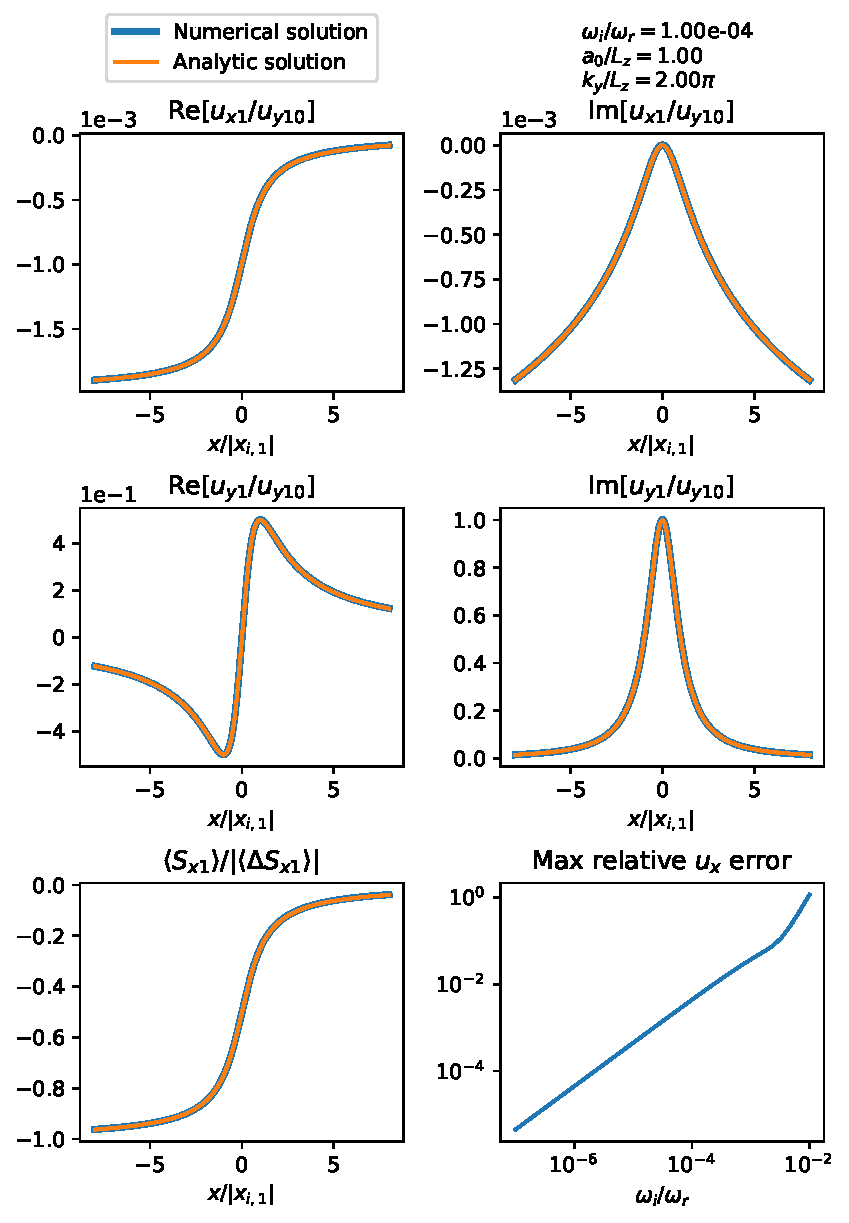
\includegraphics[width=\textwidth,height=0.85\textheight,keepaspectratio]{figures/chapter04/normal_mode_along_x_alpha=0.pdf}
    \vspace{-10pt}
    \caption{This figure shows the real and imaginary parts of $u_{x1}(x)$, $u_{y1}(x)$, as well as the Poynting flux, $\langle S_{x1}\rangle$ as a function of $x$. The bottom-right shows the maximum relative error between the numerical and analytic solutions for $u_x$ against $\omega_i$ (see Equation \ref{eq:chap_4_max_relative_ux_error}). We calculated the blue curves numerically and calculated the orange curves analytically. Note that the Poynting flux is normalised by the absolute value of the jump, $\abs{\langle\Delta S_{x1}\rangle}$, from Equation \eqref{eq:chap_4_jump_in_poynting_flux}. The code used to make this figure is available on GitHub in the following directory:\newline
    \texttt{$\rightarrow$ Python/Chapter4/normal\_mode\_along\_x\_alpha=0.py}}
    \vspace{-20pt}
    \label{fig:normal_mode_along_x_alpha=0}
\end{figure}

To check the accuracy and give a visualisation of Equations \eqref{eq:uxn_leading_order_solution}, \eqref{eq:uyn_leading_order_solution} and \eqref{eq:chap_4_avg_poy_flux_leading_order_alpha=0}, we plot these solutions and compare them with solutions calculated numerically. In the top row of Figure \ref{fig:normal_mode_along_x_alpha=0} we show the real and imaginary parts of $u_{x1}(x)$. The analytic solution was calculated using Equation \eqref{eq:uxn_leading_order_solution}. The blue curve shows the numerical solution and the orange curve shows the analytic solution using Equation \eqref{eq:uxn_leading_order_solution}. The middle row shows the real and imaginary parts of $u_{y1}(x)$. The numerical solution was calculated by rearranging Equation \eqref{eq:chap_4_uy_eqn2_alpha=0}, to give
\begin{equation}
    u_{yn}(x)=\frac{-ik_y}{\mathcal{L}_n(x)-k_y^2}\dv{u_{xn}}{x}.
\end{equation}
The analytic solution was calculated using Equation \eqref{eq:uyn_leading_order_solution}.
The bottom left plot shows the average Poynting flux directed in the $x$-direction. This was calculated using Equation \eqref{eq:chap_4_avg_poy_flux_nth_contribution} for $n=1$. To calculate $\hat{b}_{z1}(x)$ numerically we used Equation \eqref{eq:chap_4_bz_eqn2_alpha=0} to give
\begin{equation}
    \hat{b}_{zn}(x)=\frac{1}{i\omega}\qty[\pdv{u_{xn}}{x}+ik_y u_{y n}].
\end{equation}
The analytic solution was calculated using Equation \eqref{eq:chap_4_avg_poy_flux_leading_order_alpha=0}. 
% The Poynting flux is normalised by a term labelled $\langle S_{x10}\rangle$, which is given by
% \begin{equation}
%     \label{eq:Sx10}
%     \langle S_{x10}\rangle = \pi\frac{B_0^2}{\mu}\frac{u_{y10}^2x_{i,1}^2\omega}{v_A^2(x)a(x)}\,\text{sign}(x_i),
% \end{equation}
% which comes from the coefficient of Equation \eqref{eq:chap_4_jump_in_poynting_flux}.
These plots show that the analytic and numerical solutions are in approximate agreement. However, this is for $\omega_i/\omega_r = 10^{-4}$. In the bottom right, we show the maximum relative error between the analytic and numerical solutions for $u_x$ as a function of $\omega_i$. The maximum relative error is given by
\begin{equation}
    \label{eq:chap_4_max_relative_ux_error}
    \text{Max relative $u_x$ error} = \max_{|x|\le 8|x_{i,1}|} \abs{\frac{u_{x,1}^{(num)} - u_{x,1}^{(ana)}}{u_{x,1}^{(num)}}},
\end{equation}
where $u_{x,1}^{(num)}$ denotes $u_{x,1}$ calculate numerically and $u_{x,1}^{(ana)}$ denotes $u_{x,1}$ calculated analytically using Equation \eqref{eq:uxn_leading_order_solution}. The bottom-right plot shows that as $\omega_i/\omega_r$ increases, there error between the analytic and numerical solutions increases.

\section{Oblique field: Uniform density profile}
\label{sec:oblique_field_uniform_density_profile_with_line_tied_bcs}

This section aims to show how boundary layers can form if the background magnetic field is oblique to the $z=z_{min}$ and $z=z_{max}$ boundaries. For simplicity, we will model the background Alfv\'en speed as uniform, i.e. $v_A(x,z)=v_{A0}$ as this allows us to derive a simple algebraic dispersion relation. We will calculate the normal mode solution in a domain where we impose an incident Alfv\'en wave from $z>0$ and line-tied boundary conditions at $z=0$. Results from this section will be compared with results from Section \ref{sec:oblique_field_piecewise_constant_density_profile} to test the validity of imposing line-tied boundary conditions.

\subsection{Dispersion relation}

Since the background Alfv\'en speed is uniform we can derive a dispersion relation using a method very similar to that used in Section \ref{sec:mhd_waves_dispersion_relation}. The derivation here is almost identical except $\pdv*{}{y}\rightarrow\nabla_\perp$ and $\pdv*{}{z}\rightarrow\nabla_{||}$.
Eliminating $\hat{b}_x$ and $\hat{b}_{||}$ from Equations \eqref{eq:chap_4_ux_eqn1} and \eqref{eq:chap_4_u_perp_eqn1} gives
\begin{gather}
    \qty[\pdv[2]{}{t}-v_{A0}^2\nabla_{||}^2]u_x=-v_{A0}^2\pdv{\hat{b}_{||}}{x}{t}, \\
    \qty[\pdv[2]{}{t}-v_{A0}^2\nabla_{||}^2]u_\perp=-v_{A0}^2\nabla_\perp\pdv{\hat{b}_{||}}{t}.
\end{gather}
Eliminating $\hat{b}_{||}$ gives
\begin{gather}
    \label{eq:chap_4_ux_u_perp_eqn_uniform_in_x}
    \qty[\pdv[2]{}{t}-v_{A0}^2\qty(\pdv[2]{}{x}+\nabla_{||}^2)]u_x=v_A^2(z)\nabla_\perp\pdv{u_\perp}{x}, \\
    \qty[\pdv[2]{}{t}-v_{A0}^2\qty(\nabla_\perp^2+\nabla_{||}^2)]u_\perp=v_A^2(z)\nabla_\perp\pdv{u_x}{x}.
\end{gather}
For $z\ne0$,
\[\qty[\pdv[2]{}{t}-v_{A0}^2\qty(\nabla_\perp^2 + \nabla_{||}^2)]\qty[\pdv[2]{}{t}-v_{A0}^2\qty(\pdv[2]{}{x}+\nabla_{||}^2)]u_\perp=v_A^4\nabla_\perp^2 \pdv[2]{u_\perp}{x},\]
\[\implies \qty[\pdv[2]{}{t}-v_{A0}^2\nabla_{||}^2]\qty[\pdv[2]{}{t}-v_{A0}^2\qty(\pdv[2]{}{x}+\nabla_{||}^2)]u_\perp-v_{A0}^2\nabla_\perp^2\qty[\pdv[2]{}{t}-v_{A0}^2\nabla_{||}^2]u_\perp=0,\]
\begin{equation}
    \label{eq:u_perp_eqn_uniform}
    \implies \qty[\pdv[2]{}{t}-v_{A0}^2\nabla_{||}^2]\qty[\pdv[2]{}{t}-v_{A0}^2\qty(\pdv[2]{}{x}+\nabla_\perp^2+\nabla_{||}^2)]u_\perp=0.
\end{equation}
To derive the dispersion relation, assume $u_\perp$ is of the form
\[u_\perp = u_{\perp n}\exp[i(k_x x + k_y y + k_{zn} z + \omega t)]\]
Substituting this into Equation \eqref{eq:u_perp_eqn_uniform} gives the following dispersion relations
\begin{equation}
    [\omega^2+v_{A0}^2\nabla_{||n}^2][\omega^2-v_{A0}^2(k_x^2+k_y^2+k_{zn}^2)]=0,
\end{equation}
where
\begin{equation}
    \nabla_{||n} = i(k_y\sin\alpha+k_{zn}\cos\alpha).
\end{equation}
Hence, the possible values of $k_{zn}$ are
\begin{equation}
\label{eq:chap_4_oblique_field_uniform_dispersion_relation}
\begin{pmatrix}
k_{z1} \\
k_{z2} \\
k_{z3} \\
k_{z4} \\
\end{pmatrix}
=
\begin{pmatrix}
 k_{||0} / \cos\alpha - k_y\tan\alpha \\
-k_{||0} / \cos\alpha - k_y\tan\alpha \\
 i\sqrt{k_x^2+k_y^2 - k_{||0}^2} \\
-i\sqrt{k_x^2+k_y^2 - k_{||0}^2}
\end{pmatrix},
\end{equation}
where $k_{||0}$ is given by Equation \eqref{eq:k_par0}.
The first two terms, $k_{z1}$, $k_{z2}$, correspond to Alfv\'en wave solutions and $k_{z3}$, $k_{z4}$ correspond to fast wave solutions. Note that the fast wave solutions are evanescent for $k_x^2+k_y^2>k_{||0}^2$.

\subsection{Normal mode solution}

In this section, we will calculate the solution in an infinite domain where we impose an incident Alfv\'en wave from the right ($z>0$) with $\vec{u}=0$ at $z=0$. We assume the solutions are of the form 
\begin{equation}
    \label{eq:chap_4_uniform_density_full_soln}
    \begin{pmatrix}
    u_x \\
    u_\perp \\
    b_x \\
    b_\perp \\
    b_{||}
    \end{pmatrix}
    =\sum_{n=1}^4 \begin{pmatrix}
    u_{xn}\\
    u_{\perp n} \\
    b_{xn} \\
    b_{\perp n} \\
    b_{|| n}
    \end{pmatrix}
    \exp[i(k_x x + k_y y + k_{zn} z + \omega t)],
\end{equation}
where each $k_{zn}$ is given by Equation \eqref{eq:chap_4_oblique_field_uniform_dispersion_relation}.

We impose an incident Alfv\'en wave from the right by setting $u_{\perp1}=u_0$, where $u_0$ gives the incident wave amplitude. We impose the amplitude of the incident fast waves to be zero, therefore, $u_{\perp4}=0$.  From Equation \eqref{eq:chap_4_ux_u_perp_eqn_uniform_in_x} we know that
\begin{equation}
    \label{eq:uxn_oblique_field_uniform_density}
    \begin{aligned}
    u_{x n} &= \frac{-ik_x\nabla_{\perp n}}{\mathcal{L}_{n}-k_x^2}u_{\perp n} \\
    &= \hat{u}_{x n}u_{\perp n},
\end{aligned}
\end{equation}
where
\begin{gather}
    \hat{u}_{x n} = \frac{-ik_x\nabla_{\perp n}}{\mathcal{L}_{n}-k_x^2}, \\
    \mathcal{L}_{n}=\nabla_{||n}^2+k_{||0}^2, \\
    \nabla_{\perp n} = i(k_y\cos\alpha - k_{zn}\sin\alpha), \\
    \nabla_{||n} = i(k_y\sin\alpha+k_{zn}\cos\alpha).
\end{gather}
We require $u_x(x,y,0,t)=u_\perp(x,y,0,t)=0$, hence,
\begin{equation}
\begin{pmatrix}
1 & 1 \\
\hat{u}_{x2} & \hat{u}_{x3}
\end{pmatrix}
\begin{pmatrix}
u_{\perp 2} \\
u_{\perp 3} \\
\end{pmatrix}
=
-u_0
\begin{pmatrix}
1 \\
\hat{u}_{x1}
\end{pmatrix}.
\end{equation}
Hence,
\begin{equation}
    \label{eq:u_perp_n_oblique_field_uniform_density}
    \begin{pmatrix}
    u_{\perp 1} \\
    u_{\perp 2} \\
    u_{\perp 2}
    \end{pmatrix}
    = u_0
    \begin{pmatrix}
    1 \\
    -(\hat{u}_{x1}-\hat{u}_{x3})/(\hat{u}_{x2}-\hat{u}_{x3}) \\
    (\hat{u}_{x1}-\hat{u}_{x2})/(\hat{u}_{x2}-\hat{u}_{x3})
    \end{pmatrix}
\end{equation}
From Equations \eqref{eq:chap_4_bx_eqn1}, \eqref{eq:chap_4_b_perp_eqn1} and \eqref{eq:chap_4_b_par_eqn1}, we know that
\begin{gather}
    \label{eq:bxn_oblique_field_uniform_density}
    v_{A0}\hat{b}_{xn} = \frac{\nabla_{||n}}{ik_{||0}}u_{xn}, \\
    \label{eq:b_perp_n_oblique_field_uniform_density}
    v_{A0}\hat{b}_{\perp n} = \frac{\nabla_{||n}}{ik_{||0}}u_{\perp n}, \\
    \label{eq:chap_4_uniform_density_b_par0}
    v_{A0}\hat{b}_{|| n} = -\frac{1}{ik_{||0}}\qty[ik_x u_{xn}+\nabla_{\perp n} u_{\perp n}].
\end{gather}

To help visualise the solutions and to check $u_x=u_\perp=0$ at $z=0$ we plot the solutions in Figure \ref{fig:uniform_density_profile}. We choose a large value of $k_x$, namely, $k_x = 50k_{||0}$, to simulate the conditions near a singularity in a resonant absorption experiment. This means that the fast wave terms are evanescent. The plots show that for $\hat{b}_x$ and $\hat{b}_{||}$ the evanescent fast waves dominate near $z=0$. For $u_x$ and $b_{\perp}$ the evanescent fast waves and Alfv\'en waves are of a similar order near $z=0$. For $u_\perp$, the Alfv\'en waves dominate.

\begin{figure}
    \centering
    \vspace{-20pt}
    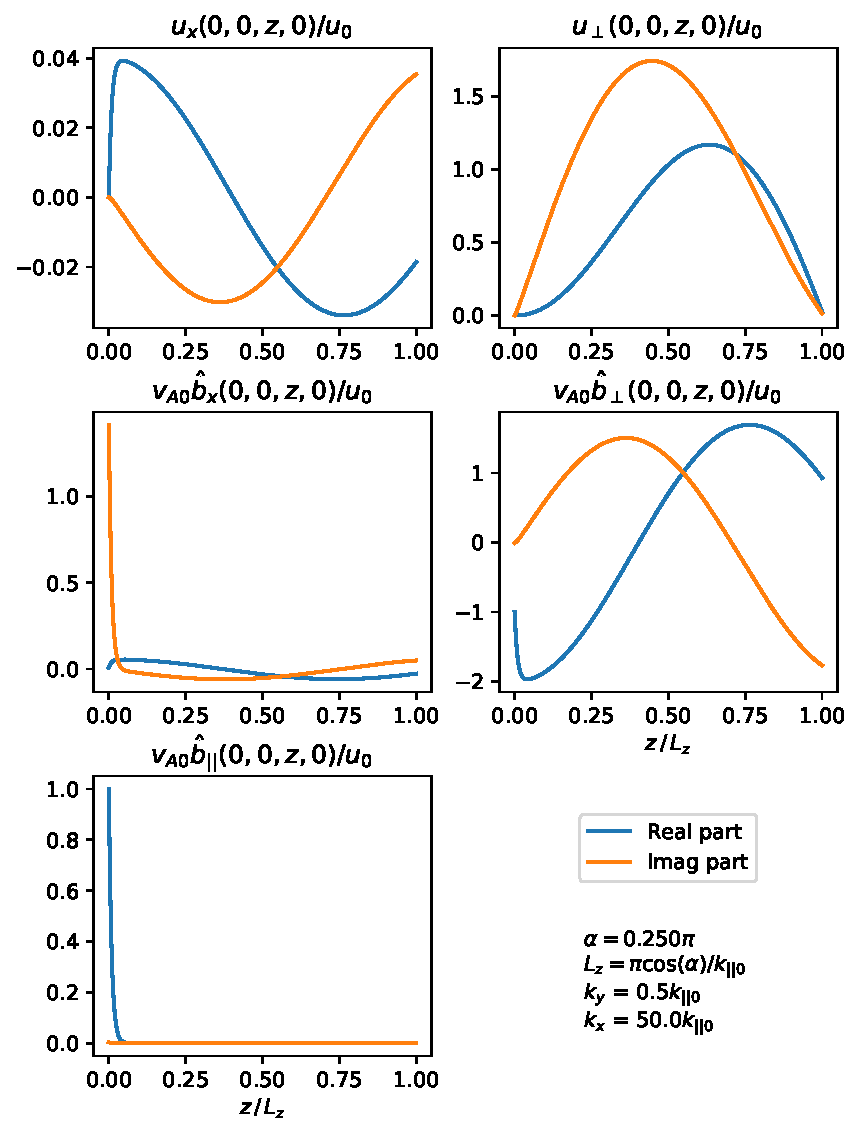
\includegraphics[width=\textwidth,height=0.9\textheight,keepaspectratio]{figures/chapter04/uniform_density_profile.pdf}
    \vspace{-10pt}
    \caption{This figure shows plots of the real and imaginary parts of $u_x$, $u_\perp$, $b_x$, $b_\perp$ and $b_{||}$ as a function of $z$. We calculated the solutions using Equations \eqref{eq:chap_4_uniform_density_full_soln}-\eqref{eq:chap_4_uniform_density_b_par0}. The code used to make this figure is available on GitHub in the following directory:\newline
    \href{https://github.com/aleksyprok/apkp_thesis/blob/main/Python/Chapter4/uniform_density_profile.py}{$\rightarrow$ Python/Chapter4/uniform\_density\_profile.py}}
    \label{fig:uniform_density_profile}
    \vspace{-20pt}
\end{figure}

Equations \eqref{eq:chap_4_uniform_density_full_soln}-\eqref{eq:chap_4_uniform_density_b_par0} give the the full set of solutions to the equations. However, we do not express the solutions in full here as they are cumbersome. We find the equations are easier to interpret if we construct series solutions by taking appropriate limits. Resonant absorption cannot occur because the background Alfv\'en speed is uniform. Therefore, singularities cannot form in our model.
In Section \ref{sec:normal_field_resonant_absorption_with_line_tied_bcs}, we showed that resonant absorption produces very short length-scales in $x$. Approaching resonant singularities, the length-scales in $x$ shrink to zero. Therefore, we are interested in the limit $k_x/k_{||0}\rightarrow \infty$. Note that for $k_x\rightarrow\infty$ the fast wave solutions are evanescent. To help us understand the effects of line-tied boundary conditions, we will now calculate asymptotic expansions for $u_{xn}$, $u_{\perp n}$, $b_{x n}$, $b_{\perp n}$ and $b_{||n}$. The maple file we use to assist the algebra can be found in the following directory:
\[\text{\href{https://github.com/aleksyprok/apkp_thesis/blob/main/Maple/Chapter4/asymptotic_expansion_uniform_va.mw}{$\rightarrow$ Maple/Chapter4/uniform\_in\_x\_vA0.mw}}.\]
To simplify the notation, let
\begin{equation}
    \hat{k}_{y0} = \frac{k_y}{k_{||0}}.
\end{equation}
The leading order asymptotic expansion for the $u_x$ coefficients is given by
\begin{gather}
    \label{eq:chap_4_oblique_ux1}
    \frac{u_{x1}}{u_0}= -\frac{\hat{k}_{y0}-\sin\alpha}{\cos\alpha}\frac{k_{||0}}{k_x} + O\qty(\frac{k_{||0}^2}{k_x^2}), \\
    \frac{u_{x2}}{u_0}= \frac{\hat{k}_{y0}+\sin\alpha}{\cos\alpha}\frac{k_{||0}}{k_x} + O\qty(\frac{k_{||0}^2}{k_x^2}), \\
    \label{eq:chap_4_oblique_ux3}
    \frac{u_{x3}}{u_0}= -2\tan\alpha\,\frac{k_{||0}}{k_x} + O\qty(\frac{k_{||0}^2}{k_x^2}).
\end{gather}
The leading order asymptotic expansion for the $u_\perp$ coefficients is given by
\begin{gather}
    \frac{u_{\perp1}}{u_0} = 1, \\
    \frac{u_{\perp2}}{u_0} = -1 + O\qty(\frac{k_{||0}}{k_x}), \\
    \frac{u_{\perp3}}{u_0} = 2i\frac{\sin^2\alpha}{\cos\alpha}\frac{k_{||0}}{k_x} + O\qty(\frac{k_{||0}^2}{k_x^2}).
\end{gather}
The $\hat{b}_x$ coefficients are given by
\begin{gather}
    \frac{v_{A0}\hat{b}_{x1}}{u_0} = -\frac{\hat{k}_{y0}-\sin\alpha}{\cos\alpha}\frac{k_{||0}}{k_x} + O\qty(\frac{k_{||0}^2}{k_x^2}), \\
    \frac{v_{A0}\hat{b}_{x2}}{u_0} = -\frac{\hat{k}_{y0}+\sin\alpha}{\cos\alpha}\frac{k_{||0}}{k_x} + O\qty(\frac{k_{||0}^2}{k_x^2}), \\
    \frac{v_{A0}\hat{b}_{x3}}{u_0} = -2i\sin\alpha + O\qty(\frac{k_{||0}}{k_x}).
\end{gather}
The $\hat{b}_\perp$ coefficients are given by
\begin{gather}
    \frac{v_{A0}\hat{b}_{\perp1}}{u_0} = 1, \\
    \frac{v_{A0}\hat{b}_{\perp2}}{u_0} = 1 + O\qty(\frac{k_{||0}}{k_x}), \\
    \frac{v_{A0}\hat{b}_{\perp3}}{u_0} = -2\sin^2\alpha + O\qty(\frac{k_{||0}}{k_x}).
\end{gather}
Finally, the $\hat{b}_{||}$ coefficients are given by
\begin{gather}
    \frac{v_{A0}\hat{b}_{||1}}{u_0} = 0, \\
    \frac{v_{A0}\hat{b}_{||2}}{u_0} = 0, \\
    \label{eq:chap_4_oblique_b_par3}
    \frac{v_{A0}\hat{b}_{||3}}{u_0} = \sin(2\alpha) + O\qty(\frac{k_{||0}}{k_x}).
\end{gather}
For the Alfv\'en wave terms the associated magnetic pressure, $b_{||}$, equals zero and this was shown in Section \ref{sec:mhd_waves_dispersion_relation}. The above equations show that to leading order the $u_x$ solution does include an evanescent fast wave term and this gives rise to the boundary layers seen in \citet{Halberstadt1993,Halberstadt1995,Arregui2003}. However, the leading order $u_\perp$ solution does not contain any fast wave terms. Note that for $b_x$ the boundary layer term dominates near $z=0$.

Now, we give a brief explanation as to why the boundary layers form. Imposing $\vec{u}=0$ at $z=0$ forces the normal component of the magnetic field, $b_z$, to be zero. For proof, consider the $z$-component of the induction equation,
\[\pdv{b_z}{t}=\vec{\hat{z}}\cdot\curl(\vec{u}\cross\vec{B}_0).\]
The curl in the $z$-direction only depends on derivatives in $x$ and $y$. Since  $\vec{u}=0=$ constant at $z=0$, the $x$ and $y$ derivatives are zero. Therefore, if $b_z$ is initially zero, it will remain zero for all time. Therefore, at $z=0$,
\[b_z = \cos\alpha b_{||} - \sin\alpha b_\perp=0,\]
rearranging gives
\[b_{||} = \tan\alpha\, b_\perp.\]
Here, $b_\perp$ gives the magnetic field component of the Alfv\'en wave and $b_{||}$ gives the magnetic pressure component of the fast wave. Hence, for $\alpha\ne0$, if there is a large-amplitude Alfv\'en wave, then there must also be a large-amplitude fast wave (for $\alpha \ne 0$). If $v_A^2(k_x^2+k_y^2)>\omega^2$, this forces the associated $k_z$ to be imaginary, which means the fast wave must be evanescent and so boundary layers will form.

Note that for $k_x\rightarrow\infty$, $k_{z3}\rightarrow ik_x$. Therefore, the time-averaged energy associated with the evanescent fast waves is proportional to $\exp(-2k_x z)$ and the total fast wave
energy is proportional to
\begin{equation}
    k_{||+}\int_0^\infty \exp(-2 k_x z) dz = \frac{k_{||+}}{2k_x}.
\end{equation}
Thus, the evanescent fast waves' energy tends to 0 as $k_x\rightarrow \infty$, for $u_0$ fixed. Hence, the evanescent fast waves will have a limited effect on the rate of resonant absorption. Since the energy associated with the boundary layers does not grow as the length-scales in $x$ get shorter, they cannot be absorbing energy. Moreover, the boundary layers cannot directly transport energy away as they are evanescent.

\section{Oblique field: Piecewise constant density profile}
\label{sec:oblique_field_piecewise_constant_density_profile}

This section aims to check if the boundary layers produced in Section \ref{sec:oblique_field_uniform_density_profile_with_line_tied_bcs} are physical or fictitious artefacts arising from the use of line-tied boundary conditions. Instead of imposing line-tied boundary conditions we use a piecewise constant density profile in $z$, i.e. the Alfv\'en speed is given by
\begin{equation}
    v_A(z) = \begin{cases}
    v_{A-}, & z < 0 \\
    v_{A+}, & z \ge 0.
    \end{cases}
\end{equation}
Note that the region $z>0$ models the corona and $z<0$ models the chromosphere, therefore, $v_{A+} > v_{A-}$ as the density in the chromosphere is higher. We impose an incident Alfv\'en wave from the region $z>0$ and then calculate the unique solution which ensures continuity of $u_x$, $u_\perp$, $\pdv*{u_x}{z}$, $\pdv*{u_\perp}{z}$ at $z=0$.

We assume the solutions are of the form
\begin{equation}
    \label{eq:oblique_field_piecewise_constant_summation}
    \begin{pmatrix}
    u_x \\
    u_\perp \\
    \hat{b}_x \\
    \hat{b}_\perp \\
    \hat{b}_{||}
    \end{pmatrix}
    =
    \sum_{n=1}^{4} \begin{pmatrix}
    u_{xn0-} \\
    u_{\perp n-} \\
    \hat{b}_{xn-} \\
    \hat{b}_{\perp n-} \\
    \hat{b}_{||n-}
    \end{pmatrix}
    \exp[i(k_x x + k_y y + k_{zn-}z + \omega t)],\ \text{for}\ z\le 0,
\end{equation}
and 
\begin{equation}
    \begin{pmatrix}
    u_x \\
    u_\perp \\
    \hat{b}_x \\
    \hat{b}_\perp \\
    \hat{b}_{||}
    \end{pmatrix}
    =
    \sum_{n=1}^{4} \begin{pmatrix}
    u_{xn+} \\
    u_{\perp n+} \\
    \hat{b}_{xn+} \\
    \hat{b}_{\perp n+} \\
    \hat{b}_{||n+}
    \end{pmatrix}
    \exp[i(k_x x + k_y y + k_{zn+}z + \omega t)],\ \text{for}\ z> 0,
\end{equation}
where
\begin{equation}
\begin{pmatrix}
k_{z1\pm} \\
k_{z2\pm} \\
k_{z3\pm} \\
k_{z4\pm} \\
\end{pmatrix}
=
\begin{pmatrix}
 k_{||\pm}/\cos\alpha - k_y\tan\alpha \\
-k_{||\pm}/\cos\alpha - k_y\tan\alpha \\
 i\sqrt{k_x^2+k_y^2 - k_{||\pm}^2} \\
-i\sqrt{k_x^2+k_y^2 - k_{||\pm}^2}
\end{pmatrix},
\end{equation}
and $k_{||\pm}$ is given by Equation \eqref{eq:k_par_pm}.

We impose an incident Alfv\'en wave from $z>0$ by setting $u_{\perp1+}=u_0$, where $u_0$ gives the incident wave amplitude. We impose the amplitude of the incident fast waves to be zero, therefore, $u_{\perp 4+}=0$. There are no incident waves from the left, therefore, $u_{\perp2-}=u_{\perp3-}=0$. From Equation \eqref{eq:chap_4_ux_u_perp_eqn_uniform_in_x} we know that
\begin{equation}
    \label{eq:uxn_pm_oblique_field_piecewise_constant_density}
    \begin{aligned}
    u_{x n\pm} &= \frac{-ik_x\nabla_{\perp n\pm}}{\mathcal{L}_{n\pm}-k_x^2}u_{\perp n\pm} \\
    &= \hat{u}_{x n\pm}u_{\perp n0\pm},
\end{aligned}
\end{equation}
where
\begin{gather}
    \hat{u}_{x n\pm} = \frac{-ik_x\nabla_{\perp n\pm}}{\mathcal{L}_{n\pm}-k_x^2}, \\
    \mathcal{L}_{n\pm}=\nabla_{||n\pm}^2+k_{||\pm}^2, \\
    \nabla_{\perp n\pm} = i(k_y\cos\alpha - k_{zn\pm}\sin\alpha),
\end{gather}
We require continuity of $u_x$, $\pdv*{u_x}{z}$, $u_\perp$ and $\pdv*{u_\perp}{z}$ at $z=0$. This gives the following equations
\[\sum_{n\in\{1,4\}}u_{xn-}=\sum_{n=1}^3u_{xn+}\implies \sum_{n\in\{1,4\}}\hat{u}_{xn-}u_{\perp n-}=\sum_{n=1}^3\hat{u}_{xn+}u_{\perp n+},\]
\[\sum_{n\in\{1,4\}}k_{zn-}u_{xn-}=\sum_{n=1}^3k_{zn+}u_{xn+}\implies \sum_{n\in\{1,4\}}k_{zn-}\hat{u}_{xn-}u_{\perp n0-}=\sum_{n=1}^3k_{zn+}\hat{u}_{xn+}u_{\perp n+},\]
\[\sum_{n\in\{1,4\}}u_{\perp n-}=\sum_{n=1}^3u_{\perp n+},\]
\[\sum_{n\in\{1,4\}}k_{zn-}u_{\perp n-}=\sum_{n=1}^3k_{zn+}u_{\perp n+}.\]
Written in matrix form, these become
\[
    \begin{pmatrix}
    \hat{u}_{x1-} & \hat{u}_{x4-} & -\hat{u}_{x2+} & -\hat{u}_{x3+} \\
    k_{z1-}\hat{u}_{x1-} & k_{z4-}\hat{u}_{x4-} & -k_{z2+}\hat{u}_{x2+} & -k_{z3+}\hat{u}_{x3+} \\
    1 & 1 & -1 &-1 \\
    k_{z1-} & k_{z4-} & -k_{z2+} & -k_{z3+}
    \end{pmatrix}
    \begin{pmatrix}
    u_{\perp 1-} \\
    u_{\perp 4-} \\
    u_{\perp 2+} \\
    u_{\perp 3+}
    \end{pmatrix}
    =u_0
    \begin{pmatrix}
    \hat{u}_{x1+} \\
    k_{z1+}\hat{u}_{x1+} \\
    1 \\
    k_{z1+}
    \end{pmatrix}.
\]
We can solve this using symbolic and numerical computing environments e.g. Maple, see Github file:
\[\text{\href{https://github.com/aleksyprok/apkp_thesis/blob/main/Maple/Chapter4/asymptotic_expansion_piecewise_constant_va_large_k_par_m.mw}{$\rightarrow$ Maple/Chapter4/asymptotic\_expansion\_piecewise\_constant\_va\_large\_k\_par\_m.mw}}.\]
From Equations \eqref{eq:chap_4_bx_eqn1}, \eqref{eq:chap_4_b_perp_eqn1} and \eqref{eq:chap_4_b_par_eqn1}, we know that
\begin{gather}
    \label{eq:bxn_pm_oblique_field_piecewise_constant_density}
    v_{A+}\hat{b}_{xn\pm} = \frac{\nabla_{||n\pm}}{ik_{||+}}u_{xn\pm}, \\
    \label{eq:b_perp_n_pm_oblique_field_piecewise_constant_density}
    v_{A+}\hat{b}_{\perp n\pm} = \frac{\nabla_{||n\pm}}{ik_{||+}}u_{\perp n\pm}, \\
    \label{eq:b_par_n_pm}
    v_{A+}\hat{b}_{|| n\pm} = -\frac{1}{ik_{||+}}\qty[ik_x u_{xn\pm}+\nabla_{\perp n\pm} u_{\perp n\pm}].
\end{gather}

\begin{figure}
    \centering
    \vspace{-20pt}
    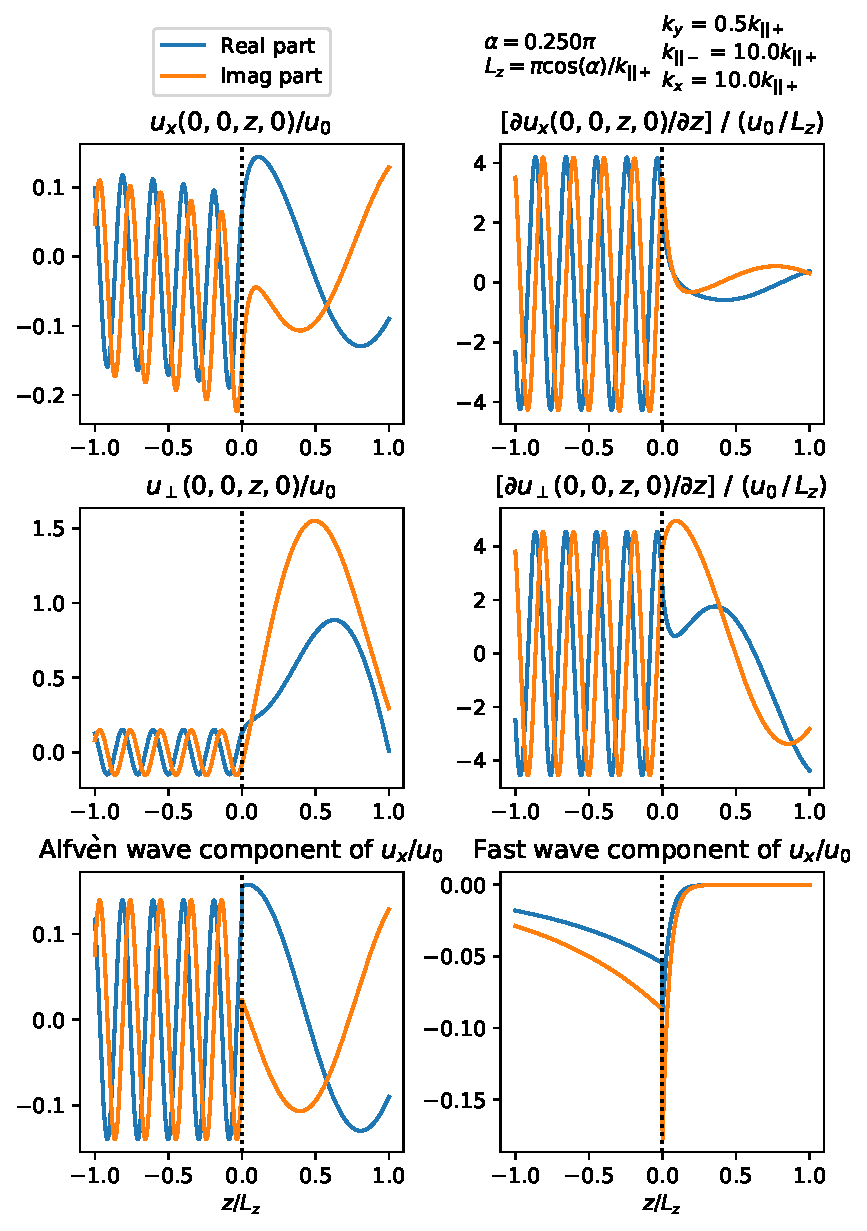
\includegraphics[width=\textwidth,height=0.85\textheight,keepaspectratio]{figures/chapter04/piecewise_constant_density_profile.pdf}
    \vspace{-10pt}
    \caption{This figure shows plots of the velocity $u_x$, $u_\perp$ and their $z$-derivatives as a function of $z$ at $x=y=t=0$. It shows that the velocities and their $z$-derivatives are continuous. The bottom row shows the Alfv\'en wave and fast components of $u_x$ separately, where the Alfv\'en wave component have wavenumbers $k_{z1\pm}$, $k_{z2\pm}$ and the fast wave component have wavenumbers $k_{z3\pm}$, $k_{z4\pm}$. The code used to make this figure is available on GitHub in the following directory:\newline
    \href{https://github.com/aleksyprok/apkp_thesis/blob/main/Python/Chapter4/piecewise_constant_density_profile.py}{$\rightarrow$ Python/Chapter4/piecewise\_constant\_density\_profile.py}}
    \vspace{-20pt}
    \label{fig:piecewise_constant_density_profile}
\end{figure}

To help check that solutions to the matrix above do indeed ensure continuity of $u_x$, $\pdv*{u_x}{z}$, $u_\perp$, $\pdv*{u_\perp}{z}$ we plot the velocities and their derivatives as a function of $z$ in Figure \ref{fig:piecewise_constant_density_profile}. Also, to help visualise the solutions we plot the Alfv\'en wave component and fast wave component for $u_x$ separately. Since $k_x^2+k_y^2>k_{||\pm}$, the fast wave component is evanescent.  We show the parameters we use in the top-right of each figure. The blue curve shows the solutions from Section \ref{sec:oblique_field_uniform_density_profile_with_line_tied_bcs} where line-tied boundary conditions ($\vec{u}=0$) are imposed at $z=0$ and $k_{||0}=k_{||+}$. The dashed orange curve shows the solution where we impose continuity of $\vec{u}$ and $\pdv*{\vec{u}}{z}$ at $z=0$ with a piecewise constant background Alfv\'en speed. In the left-hand column, $k_x=10k_{||+}$, this means that the fast waves are evanescent for $z>0$ and can propagate for $z<0$. It shows that the solutions are in good agreement and suggests that line-tied boundary conditions can provide an approximation for the solution where $z>0$. The small disagreement occurs due to line-tied boundary conditions causing perfect reflection, whereas, a finite jump in the background Alfv\'en speed results in partial reflection. In the right column, $k_x=1000k_{||+}$, this means that the fast waves are evanescent everywhere. The plots show poor agreement near $z=0$ and good agreement for $z\gg0$. They show that the model with line-tied boundary conditions can significantly overestimate the evanescent fast waves'/boundary layers' amplitude.

\begin{figure}
    \centering
    \vspace{-20pt}
    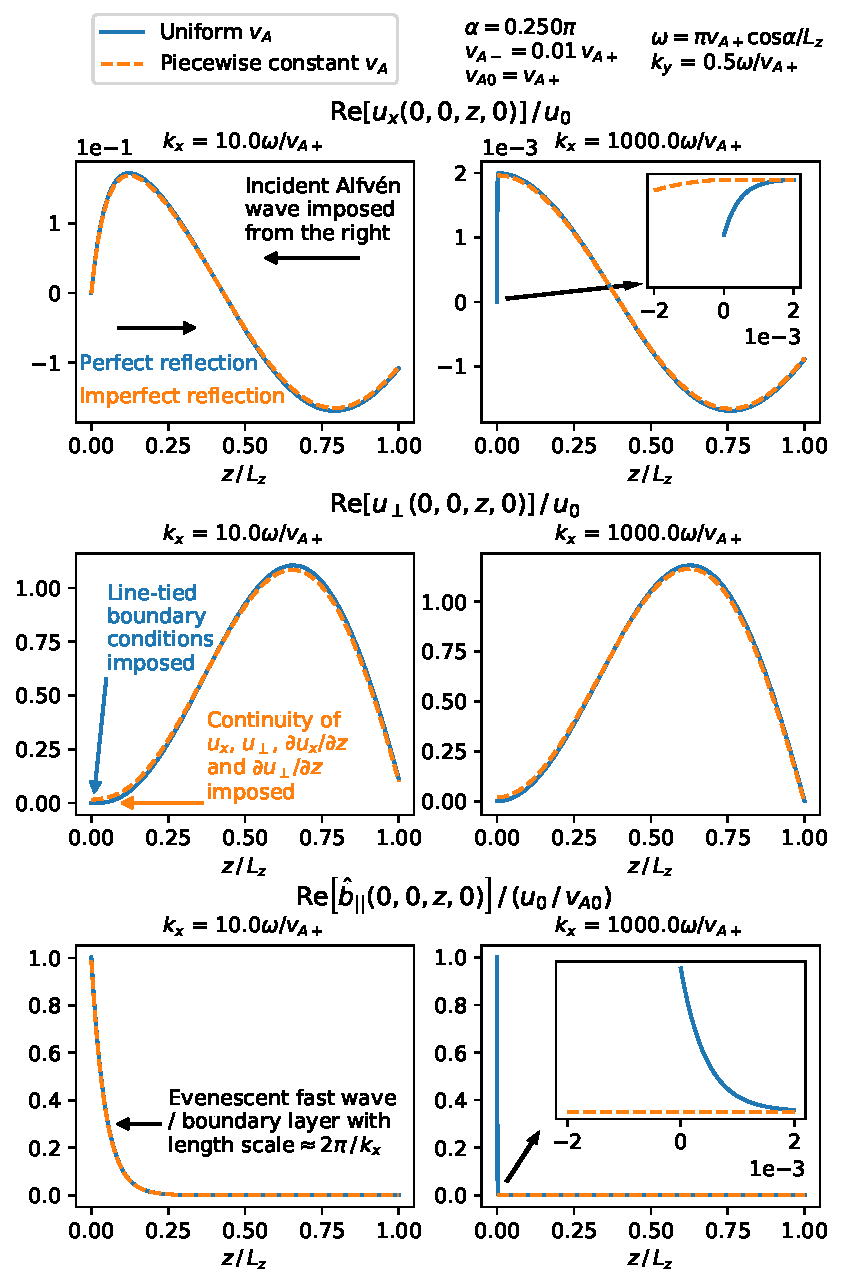
\includegraphics[width=\textwidth,height=0.8\textheight,keepaspectratio]{figures/chapter04/piecewise_constant_vs_uniform_real_part.pdf}
    \vspace{-10pt}
    \caption{This figure shows plots of the real part of $u_x$ (top row), $u_\perp$ (middle row) and $\hat{b}_{||}$ (bottom row) at $x=y=t=0$ as a function of $z$ for $k_x=10k_{||+}$ (left column) and $k_x = 1000k_{||+}$ (right column). The case where the background Alfv\'en speed is uniform and line-tied boundary conditions is imposed is shown in blue and the case where the Alfv\'en speed is piecewise constant and continuity of $\vec{u}$ is imposed is shown in dashed orange. A description of this figure is continued in the caption of Figure \ref{fig:piecewise_constant_vs_uniform_imag_part}. The code used to make this figure and Figure \ref{fig:piecewise_constant_vs_uniform_imag_part} is available on GitHub in the following directory:\newline
    \href{https://github.com/aleksyprok/apkp_thesis/blob/main/Python/Chapter4/piecewise_constant_vs_uniform.py}{$\rightarrow$ Python/Chapter4/piecewise\_constant\_vs\_uniform.py}}
    \label{fig:piecewise_constant_vs_uniform_real_part}
    \vspace{-20pt}
\end{figure}

\begin{figure}
    \centering
    \vspace{-20pt}
    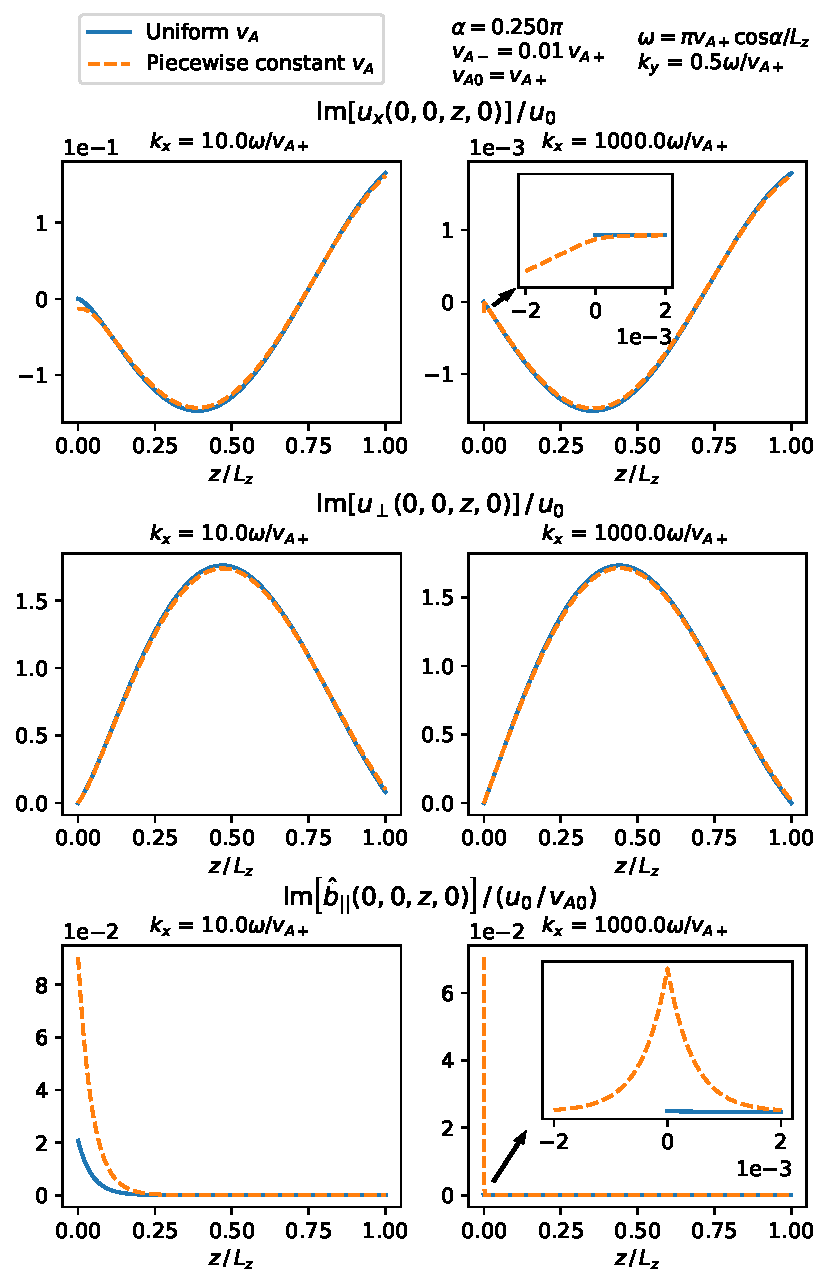
\includegraphics[width=\textwidth,height=0.8\textheight,keepaspectratio]{figures/chapter04/piecewise_constant_vs_uniform_imag_part.pdf}
    \vspace{-10pt}
    \caption{This figure is similar to Figure \ref{fig:piecewise_constant_vs_uniform_real_part} except it plots the imaginary part of each variable instead. The blue and orange curves show good agreement in the left-hand column for both figures. The small differences occur due to the waves represented by the blue curves undergoing perfect reflection and the orange waves undergoing imperfect reflection at $z=0$. The right-hand column shows less agreement between the plots, and this is because the fast waves are evanescent, whereas in the left-column the fast waves can propagate for $z<0$. Equations  \eqref{eq:uniform_alfven_wave_asymptotic_expansion_1}-\eqref{eq:uniform_fast_wave_asymptotic_expansion_2} and \eqref{eq:piecewise_alfven_wave_asymptotic_expansion_1}-\eqref{eq:piecewise_fast_wave_asymptotic_expansion_2} show that the fast wave terms in the blue solutions are of a higher order than the orange solutions.}
    \label{fig:piecewise_constant_vs_uniform_imag_part}
    \vspace{-20pt}
\end{figure}

Equations \eqref{eq:oblique_field_piecewise_constant_summation}-\eqref{eq:b_par_n_pm} give the full solution to the equations. However, the solution is too cumbersome to present directly.  To build our intuition for how the solutions change with $k_x$ we plot the real/imaginary part of $u_x$, $u_\perp$ and $\hat{b}_{||}$  as a function of $z$ at $x=y=t=0$ in Figure \ref{fig:piecewise_constant_vs_uniform_real_part}/\ref{fig:piecewise_constant_vs_uniform_imag_part} respectively. We show the parameters we use in the top-right of each figure. The blue curve shows the solutions from Section \ref{sec:oblique_field_uniform_density_profile_with_line_tied_bcs} where line-tied boundary conditions ($\vec{u}=0$) are imposed at $z=0$. The dashed orange curve shows the solution where we impose continuity of $\vec{u}$ and $\pdv*{\vec{u}}{z}$ at $z=0$ with a piecewise constant background Alfv\'en speed. In the left-hand column, $k_x=10k_{||+}$, this means that the fast waves are evanescent for $z>0$ and can propagate for $z<0$. It shows that the solutions are in good agreement and suggests that line-tied boundary conditions give a good approximation for the solution where $z>0$. The small disagreement occurs due to line-tied boundary conditions causing perfect reflection, whereas, a finite jump in the background Alfv\'en speed results in partial reflection. In the right column, $k_x=1000k_{||+}$, this means that the fast waves are evanescent everywhere. The plots show poor agreement near $z=0$ and good agreement for $z\gg0$. They show that the model with line-tied boundary conditions can significantly overestimate the evanescent fast waves'/boundary layers' amplitude.

\begin{figure}
    \centering
    \vspace{-20pt}
    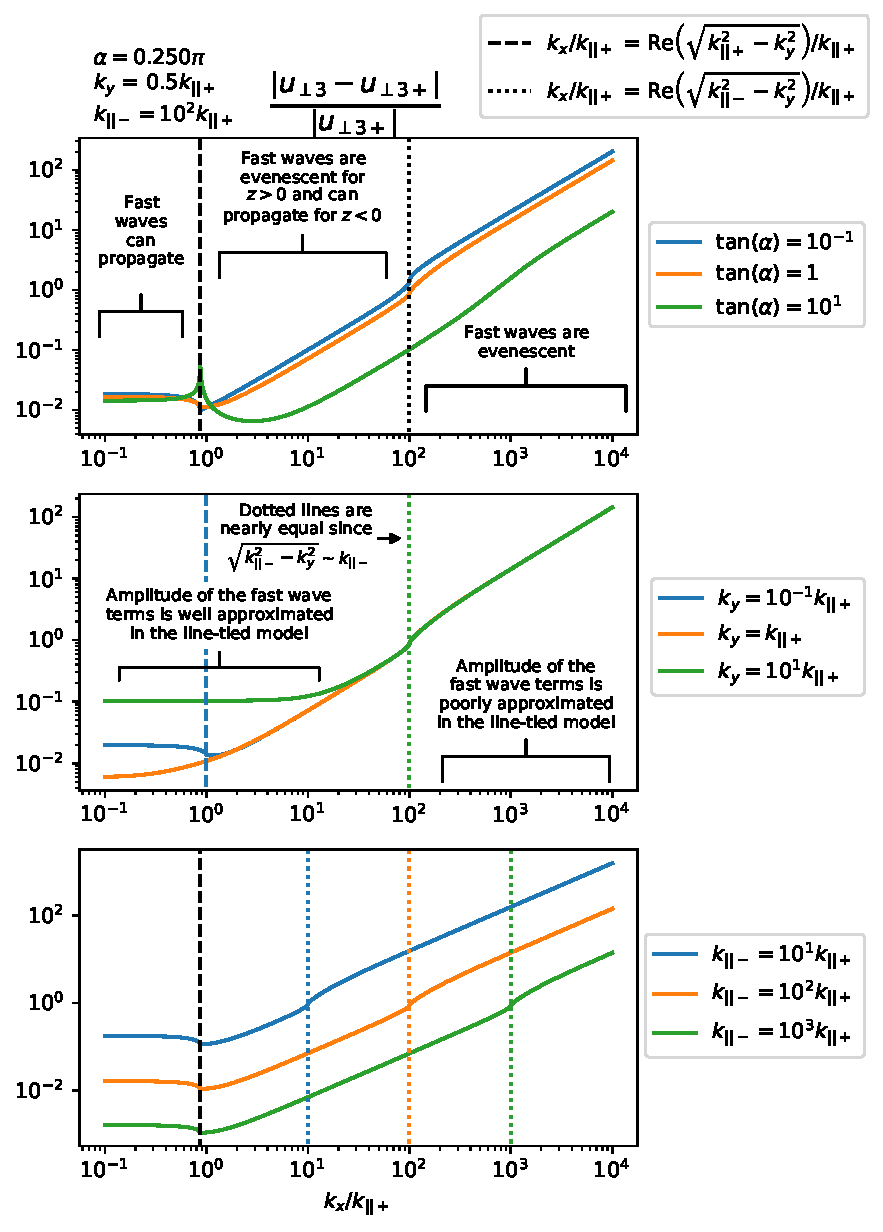
\includegraphics[width=\textwidth,height=0.8\textheight,keepaspectratio]{figures/chapter04/fast_wave_error_vs_kx.pdf}
    \vspace{-10pt}
    \caption{This figure plots the relative difference (see Equation \ref{eq:relative_difference}) introduced by using line-tied boundary conditions to estimate the size of the boundary layers as a function of $k_x$. Unless stated otherwise, we use the parameters shown in the top-left. In the top plot, the different colours correspond to different values of $\alpha$, in the middle plot they correspond to different values of $k_y$ and in the bottom plot they correspond to different values of $k_{||-}$. If $k_x$ is to the left/right of the vertical dashed lines, then the fast waves can propagate/are evanescent for $z>0$ respectively. Similarly, if $k_x$ is to the left/right of the vertical dotted lines, the fast waves can propagate/are evanescent for $z<0$ respectively. The code used to make this figure is available on GitHub in the following directory:\newline
    \href{https://github.com/aleksyprok/apkp_thesis/blob/main/Python/Chapter4/fast_wave_error_vs_kx.py}{$\rightarrow$ Python/Chapter4/fast\_wave\_error\_vs\_kx.py}}
    \label{fig:fast_wave_error_vs_kx}
    \vspace{-20pt}
\end{figure}

We have seen that depending on the value of $k_x$, our models can sometimes agree on the evanescent fast waves' amplitude and sometimes disagree strongly. Our goal now is to quantify how well the model with line-tied boundary conditions approximates the amplitude of the evanescent fast wave/boundary layer as a function of $k_x$, for the parameter space given by Equations \eqref{eq:parm_space_1}-\eqref{eq:parm_space_4}. Figure \ref{fig:fast_wave_error_vs_kx} plots the relative difference, given by,
\begin{equation}
    \label{eq:relative_difference}
    \text{relative difference} = \abs{\frac{u_{\perp3} - u_{\perp 3+}}{u_{\perp 3+}}},
\end{equation}
where $u_{\perp3}$ gives the amplitude of the fast wave component of $u_\perp$ at $z=0$ in the model where line-tied boundary conditions are imposed and $u_{\perp 3+}$ gives the amplitude in the model where a piecewise constant background Alfv\'en speed is used. Equations \eqref{eq:uxn_oblique_field_uniform_density}, \eqref{eq:bxn_oblique_field_uniform_density}, \eqref{eq:b_perp_n_oblique_field_uniform_density}, \eqref{eq:chap_4_uniform_density_b_par0} show that $u_{xn}$, $b_{xn}$, $b_{\perp n}$, $b_{|| n}$ are equal to scalar multiples of $u_{\perp n}$, similarly, Equations \eqref{eq:uxn_pm_oblique_field_piecewise_constant_density}, \eqref{eq:bxn_pm_oblique_field_piecewise_constant_density}, \eqref{eq:b_perp_n_pm_oblique_field_piecewise_constant_density}, \eqref{eq:b_par_n_pm} show that $u_{xn+}$, $b_{xn+}$, $b_{\perp n+}$, $b_{|| n+}$ are equal to the same scalar multiples of $u_{\perp n+}$ respectively (for $k_{||+}=k_{||0}$). Therefore,
\begin{equation}
    \abs{\frac{u_{\perp3} - u_{\perp 3+}}{u_{\perp +}}} = \abs{\frac{u_{x3} - u_{x 3+}}{u_{x 3+}}} = ... = \abs{\frac{b_{||3} - b_{|| 3+}}{b_{|| 3+}}}.
\end{equation}
We show all the plots as functions of $k_x$, and the parameters take values shown in the top-left (unless stated otherwise). The vertical dashed lines show where 
\[k_x = \Re\qty(\sqrt{k_{||+}^2-k_y^2})\] 
and the dotted lines show where 
\[k_x = \Re\qty(\sqrt{k_{||-}^2-k_y^2})= k_{||-} + O\qty(\frac{k_{||+}}{k_{||-}}),\]
where we assume $k_y$ satisfies Equation \eqref{eq:parm_space_ky}.
If $k_x$ is to the right of these vertical lines, then the fast waves are evanescent, and if $k_x$ is to the left, then the fast waves can propagate. The plots show that the relative difference between the models is dependent on whether the fast waves are evanescent or propagating. If $k_x \gg k_{||-}$, then the models show poor agreement and the model with line-tied boundary conditions overestimates the size of the boundary layers. On the other hand, if $k_x \ll k_{||-}$
then the models show good agreement.

Since $k_{||-}\gg k_{||+}$ it is not clear if $k_x \gg k_{||-}$, even if the waves undergo resonant absorption. Our goal now is to check if it is possible for $k_x\gg k_{||-}$ in the corona by calculating the steady-state wavenumber, $k_x^*$, for driven standing phase-mixed Alfv\'en waves in a viscous and resistive domain (note that waves during resonant absorption undergo a similar phase-mixing process). In Section \ref{sec:chap_3_open_loop} we showed $k_x^*$ is given by
\begin{equation}
    \tag{\ref{eq:kx_star}}
\begin{aligned}
    k_x^* &= \qty[\frac{6\omega}{(\eta+\nu)a}]^{1/3} \\
    &\approx 1.82 \times10^{-3} \qty[\qty(\frac{\omega}{10^{-2}\si{.s^{-1}}})\qty(\frac{10\si{.m^2.s^{-1}}}{\eta+\nu})\qty(\frac{10^6\si{.m}}{a})]^{1/3}
\end{aligned}
\end{equation}
for typical coronal values, where $\eta+\nu$ denotes the sum of the magnetic diffusivity and kinematic viscosity coefficients and $a$ is given by
\begin{equation}
    \tag{\ref{eq:length_scale_alfven_travel_time}}
    a(x) = \frac{v_A(x)}{\dv*{v_A}{x}},
\end{equation}
The Alfv\'en wavenumber parallel to the background magnetic field in the chromosphere, $k_{||-}$, is given by
\small
\begin{equation}
    \label{eq:k_par-_typical_values}
    k_{||-} = 10^{-5}\qty(\frac{\omega}{10^{-2}\si{.s^{-1}}})\qty(\frac{10^3\si{.m.s^{-1}}}{v_{A-}})\si{.m^{-1}}.
\end{equation}
\normalsize
for typical values. Comparing Equations \eqref{eq:kx_star} and \eqref{eq:k_par-_typical_values}, they show that $k_x^*$ can greatly exceed $k_{||-}$ for waves undergoing resonant absorption in the corona. However, it takes time for waves to phase-mix to such short length scales. Therefore, for early times $k_x\ll k_{||-}$ is valid and after the waves have sufficiently phase-mixed $k_x \gg k_{||+}$ is valid. 

\subsection{Asymptotic expansion: Case where \texorpdfstring{$k_{||+} \ll k_x\ll k_{||-}$}{kx||+ << kx << k||-}}

Our goal now is to calculate the asymptotic expansions for the cases where $k_{||+} \ll k_x\ll k_{||-}$ and $k_{||-}$, $k_{||+} \ll k_x$ separately. In this section we calculate the asymptotic expansions for the case where $k_{||+} \ll k_x\ll k_{||-}$ and in the next section we calculate the solution for the case where $k_{||-}$, $k_{||+} \ll k_x$. Our line-tied boundary condition solutions from Section \ref{sec:oblique_field_uniform_density_profile_with_line_tied_bcs} provide a good approximation for the case where $k_x \ll k_{||-}$ as imposing line-tied boundary conditions is equivalent to modelling the chromospehre as infinitely denser than the corona which causes $k_{||-}\rightarrow \infty$.

To simplify the notation, let
\begin{gather}
    \epsilon_- = \frac{k_x}{k_{||-}}, \\
    \epsilon_+ = \frac{k_{||+}}{k_x}, \\
    \hat{k}_{y+} = \frac{k_y}{v_{A+}}
\end{gather}
To assist with the algebra we use a maple file which can found on GitHub in the following directory:
\[\text{\href{https://github.com/aleksyprok/apkp_thesis/blob/main/Maple/Chapter4/asymptotic_expansion_piecewise_constant_va_large_k_par_m.mw}{$\rightarrow$ Maple/Chapter4/asymptotic\_expansion\_piecewise\_constant\_va\_large\_k\_par\_m.mw}}.\]
We calculate the leading order multivariate Taylor expansions (assuming $\epsilon_-,\epsilon_+\ll1$). The $u_x$ coefficients are given by
\begin{gather}
    \frac{u_{x1-}}{u_0} = -2i\sin\alpha\,\epsilon_-\epsilon_+ + O(\epsilon_-^3,\epsilon_-^2\epsilon_+,\epsilon_-\epsilon_+^2,\epsilon_+^3), \\
    \frac{u_{x4-}}{u_0} = -2\frac{\cos\alpha}{\sin\alpha}\epsilon_-^2\epsilon_+ + O(\epsilon_-^4,\epsilon_-^3\epsilon_+,...\,,\epsilon_+^4), \\
    \frac{u_{x1+}}{u_0} = -\frac{\hat{k}_{y+} - \sin\alpha}{\cos\alpha}\epsilon_+ + O(\epsilon_-^2,\epsilon_-\epsilon_+,\epsilon_+^2), \\
    \frac{u_{x2+}}{u_0} = \frac{\hat{k}_{y+} + \sin\alpha}{\cos\alpha}\epsilon_+ + O(\epsilon_-^2,\epsilon_-\epsilon_+,\epsilon_+^2), \\
    \frac{u_{x3+}}{u_0} = -2\tan\alpha\,\epsilon_+ + O(\epsilon_-^2,\epsilon_-\epsilon_+,\epsilon_+^2).
\end{gather}
The $u_\perp$ coefficients are given by
\begin{gather}
    \frac{u_{\perp1-}}{u_0}=-2i\cos\alpha\,\epsilon_-^2\epsilon_+ + O(\tiny{\epsilon_-^4,\epsilon_-^3\epsilon_+,...\,,\epsilon_+^4}) \\
    \frac{u_{\perp4-}}{u_0} = 2\cos\alpha\,\epsilon_-\epsilon_++O(\epsilon_-^2,\epsilon_-\epsilon_+,\epsilon_+^2), \\
    \frac{u_{\perp 1+}}{u_0} = 1, \\
    \frac{u_{\perp 2+}}{u_0} = -1 + O(\epsilon_-,\epsilon_+), \\
    \frac{u_{\perp 3+}}{u_0} = 2i\frac{\sin^2\alpha}{\cos\alpha}\epsilon_+ + O(\epsilon_-^2,\epsilon_-\epsilon_+,\epsilon_+^2).
\end{gather}
The $b_x$ coefficients are given by
\begin{gather}
    \frac{v_{A+}\hat{b}_{x1-}}{u_0} = -2i\sin\alpha + O(\epsilon_-,\epsilon_+), \\
    \frac{v_{A+}\hat{b}_{x4-}}{u_0} = -2\frac{\cos^2\alpha}{\sin\alpha}\epsilon_- + O(\epsilon_-^2,\epsilon_-\epsilon_+,\epsilon_+^2), \\
    \frac{v_{A+}\hat{b}_{x1+}}{u_0} = -\frac{\hat{k}_{y+} - \sin\alpha}{\cos\alpha}\epsilon_+ + O(\epsilon_-^2,\epsilon_-\epsilon_+,\epsilon_+^2), \\
    \frac{v_{A+}\hat{b}_{x2+}}{u_0} = -\frac{\hat{k}_{y+}+\sin\alpha}{\cos\alpha}\epsilon_+ + O(\epsilon_-^2,\epsilon_-\epsilon_+,\epsilon_+^2), \\
    \frac{v_{A+}\hat{b}_{x3+}}{u_0} = -2i\sin\alpha+O(\epsilon_-,\epsilon_+).
\end{gather}
The $b_\perp$ coefficients are given by
\begin{gather}
    \frac{v_{A+}b_{\perp1-}}{u_0} = -2i\cos\alpha\,\epsilon_- + O(\epsilon_-^2,\epsilon_-\epsilon_+,\epsilon_+^2), \\
    \frac{v_{A+}b_{\perp4-}}{u_0} = 2\cos^2\alpha + O(\epsilon_-,\epsilon_+), \\
    \frac{v_{A+}b_{\perp1+}}{u_0} = 1, \\
    \frac{v_{A+}b_{\perp2+}}{u_0} = 1 + O(\epsilon_-,\epsilon_+), \\
    \frac{v_{A+}b_{\perp3+}}{u_0} = -2\sin^2\alpha + O(\epsilon_-, \epsilon_+).
\end{gather}
Finally,  the $\hat{b}_{||}$ coefficients are given by
\begin{gather}
    \frac{v_{A+}b_{||1-}}{u_0} = 0, \\
    \frac{v_{A+}b_{||4-}}{u_0} = \sin(2\alpha) + O(\epsilon_-,\epsilon_+), \\
    \frac{v_{A+}b_{||1+}}{u_0} = 0, \\
    \frac{v_{A+}b_{||2+}}{u_0} = 0, \\
    \frac{v_{A+}b_{||3+}}{u_0} = \sin(2\alpha) + O(\epsilon_-, \epsilon_+).
\end{gather}
Taking the limit $\epsilon_-\rightarrow0$ we do indeed recover the asymptotic expansions derived in Section \ref{sec:oblique_field_uniform_density_profile_with_line_tied_bcs} for $z>0$ and $k_{||+}=k_{||0}$.

\subsection{Asymptotic expansion: Case where \texorpdfstring{$k_{||-}$, $k_{||+} \ll k_x$}{k||-, k||+ << kx}}

Our goal now is to calculate the solution for the case where $k_x \gg k_{||-}, k_{||+}$,
as this simulates the conditions for waves undergoing resonant absorption after they have phase-mixed to sufficiently short length scales. 
To assist with the algebra we use a maple file which can found on GitHub in the following directory:
\[\text{\href{https://github.com/aleksyprok/apkp_thesis/blob/main/Maple/Chapter4/asymptotic_expansion_piecewise_constant_va_large_kx.mw}{$\rightarrow$ Maple/Chapter4/asymptotic\_expansion\_piecewise\_constant\_va\_large\_kx.mw}}.\]
To simplify the notation, let
\begin{equation}
    r = \frac{k_{||+}}{k_{||-}}.
\end{equation}
Assuming $k_x$ is large, we calculate the leading order asymptotic expansions for the $u_x$ coefficients as
\begin{gather}
    \label{eq:oblique_field_uniform_in_x_ux10-}
    \frac{u_{x 1-}}{u_0} = -2r\frac{r \hat{k}_y-\sin\alpha}{(1+r)\cos\alpha}\frac{k_{||-}}{k_x} + O\qty(\frac{k_{||-}^2}{k_x^2}), \\
    \frac{u_{x 4-}}{u_0} = -ir(1-r)\frac{\sin\alpha}{\cos^2\alpha}\frac{k_{||-}^2}{k_x^2} + O\qty(\frac{k_{||-}^3}{k_x^3}), \\
    \frac{u_{x 1+}}{u_0} = -r\frac{\hat{k}_y-\sin\alpha}{\cos\alpha}\frac{k_{||-}}{k_x} + O\qty(\frac{k_{||-}^2}{k_x^2}), \\
    \frac{u_{x 2+}}{u_0} = r\frac{1-r}{1+r}\frac{\hat{k}_y+\sin\alpha}{\cos\alpha}\frac{k_{||-}}{k_x} + \qty(\frac{k_{||-}^2}{k_x^2}), \\
    \frac{u_{x 3+}}{u_0 } = -ir(1-r)\frac{\sin\alpha}{\cos^2\alpha}\frac{k_{||-}^2}{k_x^2} + O\qty(\frac{k_{||-}^3}{k_x^3}).
\end{gather}
The leading order asymptotic expansions for the $u_\perp$ coefficients are given by
\begin{gather}
    \frac{u_{\perp 1-}}{u_0} = \frac{2r}{r+1} + O\qty(\frac{k_{||-}^2}{k_x^2}), \\
    \label{eq:u_perp4-}
    \frac{u_{\perp 4-}}{u_0} = r(r-1)\tan^2\alpha\frac{k_{||-}^2}{k_x^2} + O\qty(\frac{k_{||-}^3}{k_x^3}), \\
    \frac{u_{\perp 1+}}{u_0} = 1, \\
    \frac{u_{\perp 2+}}{u_0} = -\frac{1-r}{1+r} + O\qty(\frac{k_{||-}^2}{k_x^2}), \\
    \frac{u_{\perp 3+}}{u_0} = -r(1-r)\tan^2\alpha \frac{k_{||-}^2}{k_x^2} + O\qty(\frac{k_{||-}^3}{k_x^3}).
\end{gather}
The leading order asymptotic expansions for the $b_x$ coefficients are given by
\begin{gather}
    \frac{v_{A+}\hat{b}_{x 1-}}{u_0} = -2\frac{r\hat{k}_y-\sin\alpha}{(1+r)\cos\alpha}\frac{k_{||-}}{k_x} + O\qty(\frac{k_{||-}^2}{k_x^2}), \\
    \frac{v_{A+}\hat{b}_{x 4-}}{u_0} = -(1-r)\tan\alpha\frac{k_{||-}}{k_x} + O\qty(\frac{k_{||-}}{k_x^2}), \\
    \frac{v_{A+}\hat{b}_{x 1+}}{u_0} = -r\frac{\hat{k}_y-\sin\alpha}{\cos\alpha}\frac{k_{||-}}{k_x} + O\qty(\frac{k_{||-}^2}{k_x^2}), \\
    \frac{v_{A+}\hat{b}_{x 2+}}{u_0} = -r\frac{1-r}{1+r}\frac{\hat{k}_y+\sin\alpha}{\cos\alpha}\frac{k_{||-}}{k_x} + O\qty(\frac{k_{||-}^2}{k_x^2}), \\
    \frac{v_{A+}\hat{b}_{x 3+}}{u_0} = (1-r)\frac{k_{||-}}{k_x} + O\qty(\frac{k_{||-}^2}{k_x^2}).
\end{gather}
The leading order asymptotic expansions for the $b_\perp$ coefficients are given by
\begin{gather}
    \frac{v_{A+}\hat{b}_{\perp 1-}}{u_0} = \frac{2}{1+r} + O\qty(\frac{k_{||-}^2}{k_x^2}), \\
    \frac{v_{A+}\hat{b}_{\perp 4-}}{u_0} = -i(1-r)\frac{\sin^2\alpha}{\cos\alpha}\frac{k_{||-}}{k_x} + O\qty(\frac{k_{||-}^2}{k_x^2}), \\
    \frac{v_{A+}\hat{b}_{\perp 1+}}{u_0} = 1, \\
    \frac{v_{A+}\hat{b}_{\perp 2+}}{u_0} = \frac{1-r}{1+r} + O\qty(\frac{k_{||-}^2}{k_x^2}), \\
    \frac{v_{A+}\hat{b}_{\perp 3+}}{u_0} = -i(1-r)\frac{\sin^2\alpha}{\cos\alpha}\frac{k_{||-}}{k_x} + O\qty(\frac{k_{||-}^2}{k_x^2}).
\end{gather}
Finally, the leading order asymptotic expansions for the $\hat{b}_{||}$ coefficients are given by
\begin{gather}
    \hat{b}_{|| 1-} = 0, \\
    \frac{v_{A+}\hat{b}_{|| 4-}}{u_0} = ir(1-r)\sin\alpha\frac{k_{||-}}{k_x} + O\qty(\frac{k_{||-}^2}{k_x^2}), \\
    \hat{b}_{|| 1+} = 0, \\
    \hat{b}_{|| 2+} = 0, \\
    \label{eq:oblique_field_uniform_in_x_b_par30+}
    \frac{v_{A+}\hat{b}_{|| 3+}}{u_0} = ir(1-r)\sin\alpha\frac{k_{||-}}{k_x} + O\qty(\frac{k_{||-}^2}{k_x^2}).
\end{gather}

Equations \eqref{eq:oblique_field_uniform_in_x_ux10-}-\eqref{eq:oblique_field_uniform_in_x_b_par30+} show that to leading order the Alfv\'en wave coefficients are given by
\begin{gather}
    \label{eq:piecewise_alfven_wave_asymptotic_expansion_1}
    \hat{b}_{||1-} = \hat{b}_{||1+} = \hat{b}_{||2+} = 0, \\
    \frac{u_{x1-}}{u_0},\ \frac{u_{x1+}}{u_0},\ \frac{u_{x2+}}{u_0},\ \frac{v_{A+}\hat{b}_{x1-}}{u_0},\ \frac{v_{A+}\hat{b}_{x1+}}{u_0},\ \frac{v_{A+}\hat{b}_{x2+}}{u_0} = O\qty(\frac{k_{||-}}{k_x}), \\
    \frac{u_{\perp1-}}{u_0},\ \frac{u_{\perp1+}}{u_0},\ \frac{u_{\perp2+}}{u_0},\ \frac{v_{A+}\hat{b}_{\perp1-}}{u_0},\ \frac{v_{A+}\hat{b}_{\perp1+}}{u_0},\ \frac{v_{A+}\hat{b}_{\perp2+}}{u_0} = O(1), \\
\end{gather}
and the fast wave coefficients are given by 
\begin{gather}
    \frac{u_{x4-}}{u_0},\ \frac{u_{x3+}}{u_0},\ \frac{u_{\perp4-}}{u_0},\ \frac{u_{\perp3+}}{u_0} = O\qty(\frac{k_{||-}^2}{k_x^2}), \\
    \label{eq:piecewise_fast_wave_asymptotic_expansion_2}
    \hat{b}_{x4-},\  \hat{b}_{x3+},\  \hat{b}_{\perp 4-},\  \hat{b}_{\perp3+},\  \hat{b}_{||4-},\  \hat{b}_{||3+},\ = \frac{u_0}{v_{A+}}O\qty(\frac{k_{||-}}{k_x}).
\end{gather}
Similarly, Equations \eqref{eq:chap_4_oblique_ux1}-\eqref{eq:chap_4_oblique_b_par3} show that to leading order 
the Alfv\'en wave coefficients are given by
\begin{gather}
    \label{eq:uniform_alfven_wave_asymptotic_expansion_1}
    \hat{b}_{||1} = \hat{b}_{||2} = 0, \\
    \frac{u_{x1}}{u_0},\ \frac{u_{x2}}{u_0},\ \frac{v_{A+}\hat{b}_{x1}}{u_0},\ \frac{v_{A+}\hat{b}_{x2}}{u_0} = O\qty(\frac{k_{||+}}{k_x}), \\
    \frac{u_{\perp1}}{u_0},\ \frac{u_{\perp 2}}{u_0},\ \frac{v_{A+}\hat{b}_{\perp1}}{u_0},\ \frac{v_{A+}\hat{b}_{\perp2}}{u_0} = O(1),
\end{gather}
and the fast wave coefficients are given by
\begin{gather}
    \frac{u_{x3}}{u_0},\ \frac{u_{\perp 3}}{u_0} = O\qty(\frac{k_{||+}}{k_x}), \\
    \label{eq:uniform_fast_wave_asymptotic_expansion_2}
    \frac{v_{A+}\hat{b}_{x3}}{u_0},\ \frac{v_{A+}\hat{b}_{\perp3}}{u_0},\ \frac{v_{A+}\hat{b}_{||3}}{u_0} = O(1).
\end{gather}
This shows that imposing line-tied boundary conditions does not change the order in $k_x$ of the Alfv\'en wave terms, however, it can increase the order of the fast wave terms by a factor $k_x$. These results suggest that imposing line-tied boundary conditions can cause the model to significantly overestimate the amplitude of the evanescent fast waves/boundary layers for $\alpha\ne0$.
Equations \eqref{eq:piecewise_alfven_wave_asymptotic_expansion_1}-\eqref{eq:piecewise_fast_wave_asymptotic_expansion_2} show that the leading order velocity does not contain any fast-wave terms. Compare this with Equations \eqref{eq:uniform_alfven_wave_asymptotic_expansion_1}-\eqref{eq:uniform_fast_wave_asymptotic_expansion_2}, which show that $u_x$ does contain a fast wave component to leading order. Therefore, for a steady-state solution in a resonant absorption experiment, the fast wave components for $u_x$ and $u_\perp$ should be negligible compared with Alfv\'en wave components near the singularities, provided line-tied boundary conditions are not imposed. In the next section we verify this claim. It is quite counter-intuitive that the length-scales parallel to the chromosphere/corona interface, e.g. $k_x$, can have such a large effect on the validity of line-tied boundary conditions. Our goal now is to give an intuitive explanation for why this is. Imposing line-tied boundary conditions is in some sense equivalent to modelling the chromosome as infinitely denser than the corona, i.e. setting $k_{||-}\rightarrow \infty$. Therefore, imposing line-tied boundary conditions forces the fast waves in the chromosphere to be propagating waves. Propagating waves have a sinusoidal profile while evanescent waves have an exponential profile. This has important implications for ensuring continuity of velocity and its derivative at the chromosome/corona interface and explains why the line-tied solution can be so different to the solution with a piecewise constant density profile at the interface.

% Comparing Equations \eqref{eq:piecewise_alfven_wave_asymptotic_expansion_1}-\eqref{eq:piecewise_fast_wave_asymptotic_expansion_2} with Equations \eqref{eq:uniform_alfven_wave_asymptotic_expansion_1}-\eqref{eq:uniform_fast_wave_asymptotic_expansion_2}, we see that the Alfv\'en wave terms retain the same order and the fast wave terms are reduced here by a factor $k_x$. These results suggest that imposing line-tied boundary conditions can cause the model to significantly overestimate the amplitude of the evanescent fast waves / boundary layers for $\alpha\ne0$.
% Equations \eqref{eq:piecewise_alfven_wave_asymptotic_expansion_1}-\eqref{eq:piecewise_fast_wave_asymptotic_expansion_2} show that the leading order velocity does not contain any fast-wave terms. Compare this with Equations \eqref{eq:uniform_alfven_wave_asymptotic_expansion_1}-\eqref{eq:uniform_fast_wave_asymptotic_expansion_2}, which show that $u_x$ does contain a fast wave component to leading order. Therefore, for a steady-state solution in a resonant absorption experiment, the fast wave components for $u_x$ and $u_\perp$ should be negligible compared with Alfv\'en wave components near the singularities, provided line-tied boundary conditions are not imposed. In the next section we verify this claim.

% Comparing the leading term in the asymptotic expansion for $u_{\perp40-}$ with $u_0$, we estimate that the velocity amplitude of the fast waves terms is negligible compared with the amplitude of the Alfv\'en wave terms provided
% % \[u_0 \gg u_0\omega^2\tan^2\alpha\frac{|v_{A+}-v_{A-}|}{v_{A+}^2v_{A-}}\frac{1}{k_x^2},\]
% % \[\implies k_x^2 \gg \omega^2\tan^2\alpha\frac{|v_{A+}-v_{A-}|}{v_{A+}^2v_{A-}},\]
% % for $v_{A-}\ll v_{A+}$ this gives
% \begin{equation}
%     \label{eq:chap_4_kx_condition}
%     k_x^2 \gg \frac{\omega^2\tan^2\alpha}{v_{A+}v_{A-}},
% \end{equation}
% where we assume that $v_{A-}\ll v_{A+}$. Our goal now is to verify if this condition is satisfied for realistic coronal parameters. We can approximate the growth in $k_x$ due to phase mixing by rearranging Equation \eqref{eq:kx_star} to give
% \begin{equation}
%     \label{eq:kx_growth}
%     k_x = \frac{1}{a}\frac{t}{\tau_A},
% \end{equation}
% where 
% \begin{gather}
%     \tag{\ref{eq:chap_3_alfven_travel_time}}
%     \tau_A = \frac{L}{v_A}, \\
%     \tag{\ref{eq:length_scale_alfven_travel_time}}
%     a = \frac{v_A}{\dv*{v_A}{x}},
% \end{gather}
% and $L$ gives the length of the coronal loop. Rearranging Equation \eqref{eq:chap_4_kx_condition} and substituting Equation \eqref{eq:kx_growth}  we require
% \begin{equation}
%     \begin{aligned}
%         1 &\gg \frac{\omega^2 \tan^2\alpha}{v_{A+}v_{A-}k_x^2} \\
%          &\approx 10^{-1}\qty(\frac{a}{10^6\si{.m}})^2\qty(\frac{\omega}{10^{-2}\si{.Hz}})^2\qty(\frac{10^6\si{.m.s^{-1}}}{v_{A+}})\qty(\frac{10^3\si{.m.s^{-1}}}{v_{A-}})\tan^2\alpha,
%     \end{aligned}
% \end{equation}
% where we substituted $t=\tau_A$. Note that \citet{Roberts2019} estimates resonant absorption causes waves to decay on a timescale of about 20 Alfv\'en travel times, $\tau_A$. Moreover, this assumes that the waves initially have $k_x=0$, in reality, $k_x$ will usually have some non-zero value before the resonant absorption occurs. The above equation shows that Equation \eqref{eq:chap_4_kx_condition}, is usually satisfied after one Alfv\'en travel time in a typical coronal loop. We use a value of $a=1\si{.Mm}$ because \citet{Klimchuk2015} shows that coronal loops have a characteristic diameter of approximately $1.5\si{.Mm}$. If we assume a density contrast, $\rho_i/\rho_o=2$, \citep{Hood2013,Pascoe2013} where $\rho_i$ gives the density inside a loop and $\rho_o$ gives the density outside a loop then this gives a length-scale $a\approx1\si{.Mm}$.

% The asymptotic expansions show that to leading order the velocity does not contain any fast-wave terms. Compare this with the asymptotic expansions (see Equations \ref{eq:oblique_field_uniform_in_x_ux10-}-\ref{eq:oblique_field_uniform_in_x_b_par30+}) from the previous section which showed $u_x$ does contain a fast wave to leading order. This suggests that imposing line-tied boundary conditions can cause the model to overestimate greatly the amplitude of the boundary layers. It also suggests that in a resonant absorption experiment the fast wave terms for $u_x$ and $u_\perp$ should be negligible near the singularities. We verify this claim in the next section. 

\section{Oblique field: Resonant absorption}
\label{sec:oblique_field_resonant_absorption}

In this section, we allow the Alfv\'en speed to be dependent on $x$ as this enables resonant absorption to occur. Our goal in this section is to verify our claim, (see end of Section \ref{sec:oblique_field_piecewise_constant_density_profile}) that the velocity amplitude of the boundary layers should be negligible near the singularity in a resonant absorption experiment.

\subsection{Model and equations}

The Alfv\'en speed is given by $v_A(x,z)=\hat{v}_A(x)v_A(0,z)$, where $v_A(0,z)$ is given by Equation \eqref{eq:chap_4_vA(0,z)} and $\hat{v}_A(x)$ is an arbitrary function of $x$ satisfying $\hat{v}_A(x)=1$. 

We seek normal mode solutions and assume the variables are of the form
\[f(x,y,z,t) = f'(x,z)\exp\{i[k_\perp(\cos\alpha\,y - \sin\alpha\,z)+\omega t]\}.\]
Note that
\[\nabla_\perp f(x,y,z,t) = \exp\{i[k_\perp(\cos\alpha\,y - \sin\alpha\,z)+\omega t]\}\qty(ik_\perp - \sin\alpha\pdv{}{z})f',\]
\[\nabla_{||} f(x,y,z,t) = \exp\{i[k_\perp(\cos\alpha\,y - \sin\alpha\,z)+\omega t]\}\cos\alpha\pdv{f'}{z} .\]
Therefore, Equations \eqref{eq:chap_4_ux_eqn1}-\eqref{eq:chap_4_b_par_eqn1} can be simplified to
\begin{gather}
    i\omega u_x'=v_A^2(x,z)\qty[\nabla_{||}'\hat{b}_x' - \pdv{\hat{b}_{||}'}{x}], \\
    i\omega u_\perp'=v_A^2(x,z)\qty[\nabla_{||}'\hat{b}_\perp'-\nabla_\perp' \hat{b}_{||}'], \\
    i\omega \hat{b}_x'=\nabla_{||}'u_x', \\
    i\omega \hat{b}_\perp'=\nabla_{||}'u_{\perp}', \\
    i\omega \hat{b}_{||}'=-\qty[\pdv{u_x'}{x}+\nabla_\perp' u_{\perp}'].
\end{gather}
where
\begin{gather}
    \nabla_\perp' = \qty(ik_\perp - \sin\alpha\pdv{}{z}), \\
    \nabla_{||}' = \cos\alpha\pdv{}{z}.
\end{gather}
Eliminating $\hat{b}_x'$ and $\hat{b}_\perp'$ gives
\begin{gather}
    \label{eq:chap4_ux_eqn_DAE}
    \pdv{u_x'}{x} = -\qty[i\omega \hat{b}_{||'} + \nabla_\perp' u_\perp'], \\
    \label{eq:chap4_b_par_eqn_DAE}
    \pdv{\hat{b}_{||}'}{x} = -\frac{i}{\omega}\mathcal{L}'u_x', \\
    \label{eq:chap4_u_perp_eqn_DAE}
    \mathcal{L}'u_\perp' = i\omega \nabla_\perp' \hat{b}_{||}',
\end{gather}
% and for $z\ne0$
% \begin{equation}
%     \label{eq:chap4_nabla_perp_u_perp_eqn_DAE}
%     \mathcal{L}'\nabla_\perp' u_\perp' = i\omega \nabla_\perp'^2 \hat{b}_{||}',
% \end{equation}
where
\begin{equation}
    \mathcal{L}' = \nabla_{||}'^2+\frac{\omega^2}{v_A^2(x,z)}.
\end{equation}

Note that the $z$ domain is given by $-L_z\le z\le L_z$. In this section, we impose periodic boundary conditions such that 
\begin{gather}
    \label{eq:chap_4_periodic_bcs}
    u_x'(x,-L_z)=u_x'(x,L_z),\quad \left.\pdv{u_x'}{z}\right|_{z=-L_z}=\left.\pdv{u_x'}{z}\right|_{z=L_z}, \\
    b_{||}'(x,-L_z)=b_{||}'(x,L_z),\quad \left.\pdv{b_{||}'}{z}\right|_{z=-L_z}=\left.\pdv{b_{||}'}{z}\right|_{z=L_z}, \\
    u_\perp'(x,-L_z)=u_\perp'(x,L_z),\quad \left.\pdv{u_\perp'}{z}\right|_{z=-L_z}=\left.\pdv{u_\perp'}{z}\right|_{z=L_z}.
\end{gather}
We choose these boundary conditions because they can be easily implemented both numerically and analytically without introducing fictitious boundary layers. Our model approximates a loop in the corona which goes into the chromosphere then back into the corona and so on.

\subsection{Eigenfunctions and eigenfrequencies}

To help solve Equations \eqref{eq:chap4_ux_eqn_DAE}-\eqref{eq:chap4_u_perp_eqn_DAE} we assume the solutions are of the form
\begin{gather}
    \label{eq:chap_4_oblique_ux_eigenfunction_expansion}
    u_x'(x,z) = u_{x0}^{(1)}(x)\phi_0(z) + \sum_{n=1}^\infty u_{xn}^{(1)}(x)\phi_n(z) + u_{xn}^{(2)}(x)\varphi_n(z), \\
    \label{eq:chap_4_oblique_b_par_eigenfunction_expansion}
    b_{||}'(x,z) = b_{||0}^{(1)}(x)\phi_0(z) + \sum_{n=1}^\infty b_{||n}^{(1)}(x)\phi_n(z) + b_{||n}^{(2)}(x)\varphi_n(z), \\
    \label{eq:chap_4_oblique_u_perp_eigenfunction_expansion}
    u_\perp'(x,z) = u_{\perp0}^{(1)}(x)\phi_0(z) + \sum_{n=1}^\infty u_{\perp n}^{(1)}(x)\phi_n(z) + u_{\perp n}^{(2)}(x)\varphi_n(z),
\end{gather}
where $\phi_n$, $\varphi_n$ are eigenfunctions, with eigenfrequencies, $\omega_n$, $\varpi_n$, respectively. The eigenfunctions satisfy the following Sturm-Liouville equations,
\[\qty[\nabla_{||}'^2+\frac{\omega_n^2}{v_A^2(0,z)}]\phi_n(z)=0,\]
\[\qty[\nabla_{||}'^2+\frac{{\varpi}_n^2}{v_A^2(0,z)}]\varphi_n(z)=0,\]
as well as the periodic boundary conditions, see Equation \eqref{eq:chap_4_periodic_bcs}.

By symmetry, we assume the eigenfunctions are of the form
\begin{gather}
\phi_n(z)=A_n\begin{cases}
a_n\cos[k_{zn-} (z+l_z)], & z < 0, \\
c_n\cos[k_{zn+} (z-l_z)], & z \ge 0, \\
\end{cases} \\
\varphi_n(z)=B_n\begin{cases}
b_n\sin[\bar{k}_{zn-} (z+l_z)], & z < 0, \\
d_n\sin[\bar{k}_{zn+} (z-l_z)], & z \ge 0, \\
\end{cases}
\end{gather}
where $a_n$, $b_n$, $c_n$, $d_n$ are constants, $L_z = 2l_z$ and
\begin{gather}
    k_{zn\pm} = \frac{\omega_n}{v_{A\pm}\cos\alpha}, \\
    \bar{k}_{zn\pm} = \frac{\varpi_n}{v_{A\pm}\cos\alpha}.
\end{gather}
Hence
\begin{gather}
    \dv{\phi_n}{z}=A_n\begin{cases}
    -a_nk_{zn-}\sin[k_{zn-} (z+l_z)], & z < 0, \\
    -c_nk_{zn+}\sin[k_{zn+} (z-l_z)], & z \ge 0, \\
    \end{cases} \\
    \dv{\varphi_n}{z}=B_n\begin{cases}
    b_n\bar{k}_{zn+}\cos[\bar{k}_{zn+} (z+l_z)], & z < 0, \\
    d_n\bar{k}_{zn+}\cos[\bar{k}_{zn+} (z-l_z)], & z \ge 0. \\
    \end{cases}
\end{gather}
We require continuity of $\phi_n$, $\varphi_n$, $\dv*{\phi_n}{z}$, $\dv*{\varphi_n}{z}$ at $z=0$ and $z=\pm L_z$, this gives the following equations
\begin{gather}
\begin{pmatrix}
\cos(k_{zn-}l_z) & -\cos(k_{zn+}l_z) \\
k_{zn-}\sin(k_{zn-}l_z) & k_{zn+}\sin(k_{zn+}l_z)
\end{pmatrix}
\begin{pmatrix}
a_n \\
c_n
\end{pmatrix}
=
\begin{pmatrix}
0 \\
0
\end{pmatrix}, \\
\begin{pmatrix}
\sin(\bar{k}_{zn-}l_z) & \sin(\bar{k}_{zn+}l_z) \\
\bar{k}_{zn-}\cos(\bar{k}_{zn-}l_z) & -\bar{k}_{zn+}\cos(\bar{k}_{zn+}l_z)
\end{pmatrix}
\begin{pmatrix}
b_n \\
d_n
\end{pmatrix}
=
\begin{pmatrix}
0 \\
0
\end{pmatrix}.
\end{gather}
For non-trivial solutions to exist, $\omega_n$, $\varpi_n$ must satisfy
\begin{gather}
\label{eq:omega_n_eqn}
k_{zn+}\sin(k_{zn+}l_z)\cos(k_{zn-}l_z)+k_{zn-}\sin(k_{zn-}l_z)\cos(k_{zn+}l_z)=0, \\
\label{eq:varpi_n_eqn}
\bar{k}_{zn+}\sin(\bar{k}_{zn-}l_z)\cos(\bar{k}_{zn+}l_z)+\bar{k}_{zn-}\sin(\bar{k}_{zn+}l_z)\cos(\bar{k}_{zn-}l_z)=0.
\end{gather}
These equations define, $\omega_n$, $\varpi_n$ and we order them such that
\begin{equation}
    \omega_0<\omega_1<\omega_2...,\quad \varpi_0<\varpi_1<\varpi_2...\,,
\end{equation}
where $\omega_0=\varpi_0=0$.

Note that if $l_z=n\pi/k_{zn+}$ and $l_z=n\pi/\bar{k}_{zn+}$ the above equations simplify to
\[k_{zn-}\sin\qty(n\pi\frac{k_{zn-}}{k_{zn+}})(-1)^n=0,\quad \bar{k}_{zn+}\sin\qty(n\pi\frac{\bar{k}_{zn-}}{\bar{k}_{zn+}})(-1)^n=0,\]
which is satisfied for $v_{A+}/v_{A-}=m$, where $m$ is an integer.
If $l_z=(2n+1)\pi/(2k_{zn+})$ and $l_z=(2n+1)\pi/(2\bar{k}_{zn+})$ the above equations simplify to
\[k_{zn+}(-1)^n\cos\qty(\frac{1}{2}(2n+1)\pi\frac{k_{zn-}}{k_{zn+}})=0,\quad
\bar{k}_{zn-}(-1)^n\cos\qty(\frac{1}{2}(2n+1)\pi\frac{k_{zn-}}{k_{zn+}})=0.\]
which is satisfied for $v_{A+}/v_{A-}=m$, where $m$ is an odd integer. Therefore, for $v_{A+}/v_{A-}=m$, where $m$ is an odd positive integer, a subset of the eigenvalues are given by
\begin{equation}
    \label{eq:eigenfrequencies_for_odd_integer}
    \omega_j=\varpi_j=k\pi\frac{v_{A+}}{L_z}\cos\alpha,
\end{equation}
where $j = [(m-1)/2 + 1]k$ and $k\in\mathds{N}$.

If $\omega_n$, $\varpi_n$ satisfy Equations \eqref{eq:omega_n_eqn} and \eqref{eq:varpi_n_eqn}, then the boundary conditions and continuity conditions are ensured if
\begin{gather}
a_n = \begin{cases}
\cos(k_{zn+} l_z), & \cos(k_{zn+} l_z) \ne 0, \\
k_{zn+}\sin(k_{zn+} l_z), & \cos(k_{zn+} l_z) = 0, \\
\end{cases} \\
c_n = \begin{cases}
\cos(k_{zn-} l_z), & \cos(k_{zn-} l_z) \ne 0, \\
-k_{zn-}\sin(k_{zn-} l_z), & \cos(k_{zn-} l_z) = 0, \\
\end{cases} \\
b_n = \begin{cases}
\sin(\bar{k}_{zn+} l_z), & \sin(\bar{k}_{zn+} l_z) \ne 0, \\
\bar{k}_{zn+}\cos(\bar{k}_{zn+} l_z), & \sin(\bar{k}_{zn+} l_z) = 0, \\
\end{cases} \\
d_n = \begin{cases}
-\sin(\bar{k}_{zn-} l_z), & \sin(\bar{k}_{zn-} l_z) \ne 0, \\
\bar{k}_{zn-}\cos(\bar{k}_{zn-} l_z), & \sin(\bar{k}_{zn-} l_z) = 0. \\
\end{cases}
\end{gather}

Let $\Big\langle f_n(z), f_m(z) \Big\rangle$ denote the following inner product
\begin{equation}
    \Big\langle f_n(z), f_m(z) \Big\rangle = \frac{v_{A+}^2}{L_z}\int_{-L_z}^{L_z} \frac{f_n(z)f_m(z)}{v_A^2(0,z)}dz.
\end{equation}
By Sturm–Liouville theory, the eigenfunctions are orthogonal to each other over this inner product, hence,
\begin{equation}
    \Big\langle \phi_n(z), \varphi_m(z) \Big\rangle = 0.
\end{equation}
We normalise such that
\begin{equation}
    \Big\langle \phi_n(z), \phi_m(z) \Big\rangle = \Big\langle \varphi_n(z), \varphi_m(z) \Big\rangle = \delta_{nm},
\end{equation}
where $\delta_{nm}$ is the Kronecker delta.
Note that
\begin{gather}
    \begin{aligned}
    \frac{L_z}{v_{A+}^2}\frac{\langle \phi_n, \phi_n \rangle}{A_n^2} &= 2\int_{0}^{l_z} \frac{a_n^2}{v_{A-}^2}\cos^2(k_{zn-}z) + \frac{c_n^2}{v_{A+}^2}\cos^2(k_{zn+}z)dz \\
    &=\Bigg\{\frac{a_n^2}{2v_{A-}^2k_{zn-}}\Big[2k_{zn-}z+\sin(2k_{zn-}z)\Big]\\
    &+\frac{c_n^2}{2v_{A+}^2k_{zn+}}\Big[2k_{zn+}z+\sin(2k_{zn+}z)\Big]\Bigg\}_0^{l_z} \\
    &=\frac{a_n^2}{2v_{A-}^2k_{zn-}}\Big[2k_{zn-}l_z+\sin(2k_{zn-}l_z)\Big] \\
    &+\frac{c_n^2}{2v_{A+}^2k_{zn+}}\Big[2k_{zn+}l_z+\sin(2k_{zn+}l_z)\Big],
    \end{aligned} \\
    \begin{aligned}
    \frac{L_z}{v_{A+}^2}\frac{\langle \varphi_n, \varphi_n \rangle}{B_n^2} &=
    \frac{b_n^2}{2v_{A-}^2\bar{k}_{zn-}}\Big[2\bar{k}_{zn-}l_z-\sin(2\bar{k}_{zn-}l_z)\Big]\\
    &+ \frac{b_n^2}{2v_{A-}^2\bar{k}_{zn-}}\Big[2\bar{k}_{zn-}l_z-\sin(2\bar{k}_{zn-}l_z)\Big].
    \end{aligned}
\end{gather}
Hence,
\begin{gather}
    \begin{aligned}
    A_n = \frac{\sqrt{L_z}}{v_{A+}}\Bigg(&\frac{a_n^2}{2v_{A-}^2k_{zn-}}\Big[2k_{zn-}l_z+\sin(2k_{zn-}l_z)\Big] + \\
    &\frac{c_n^2}{2v_{A+}^2k_{zn+}}\Big[2k_{zn+}l_z+\sin(2k_{zn+}l_z)\Big] \Bigg)^{-1/2},
    \end{aligned} \\
    \begin{aligned}
    B_n = \frac{\sqrt{L_z}}{v_{A+}}\Bigg(&\frac{b_n^2}{2v_{A-}^2\bar{k}_{zn-}}\Big[2\bar{k}_{zn-}l_z-\sin(2\bar{k}_{zn-}l_z)\Big] + \\
    & \frac{b_n^2}{2v_{A-}^2\bar{k}_{zn-}}\Big[2\bar{k}_{zn-}l_z-\sin(2\bar{k}_{zn-}l_z)\Big] \Bigg)^{-1/2}.
    \end{aligned}
\end{gather}

\begin{figure}
    \centering
    \vspace{-20pt}
    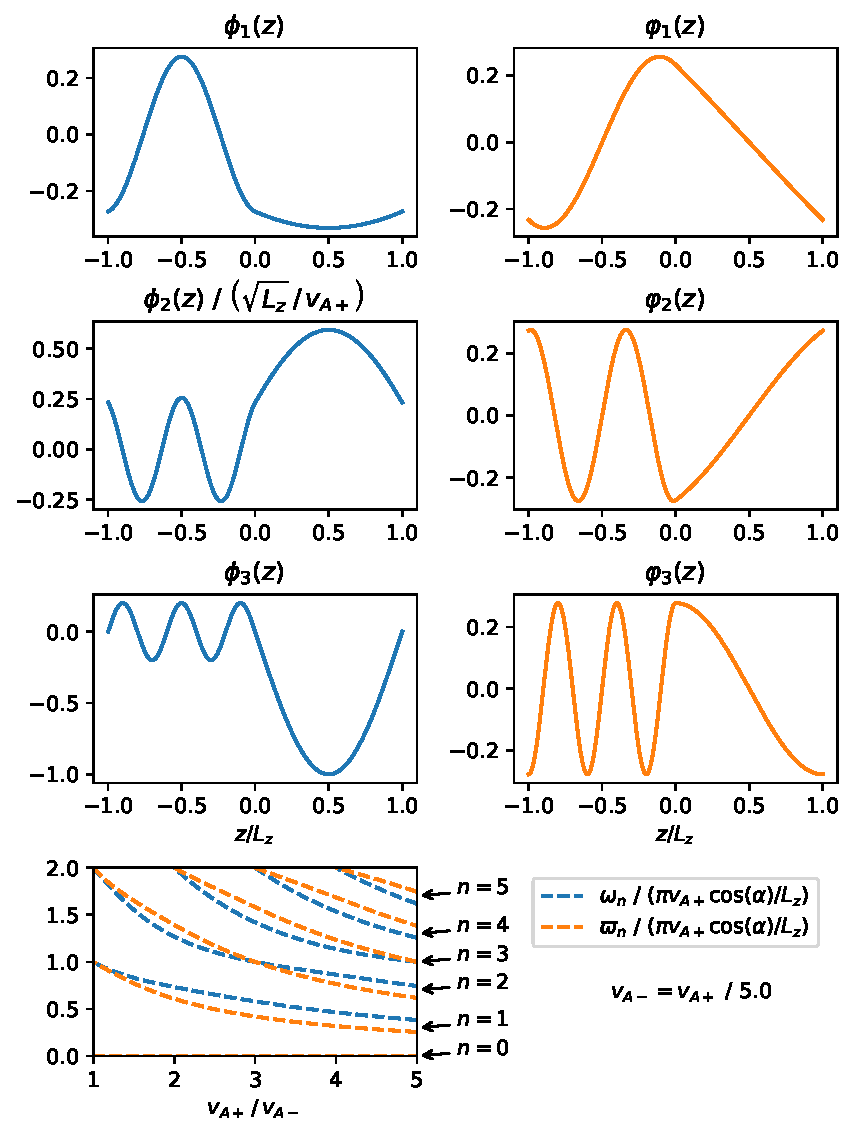
\includegraphics[width=\textwidth,height=0.9\textheight,keepaspectratio]{figures/chapter04/eigenfunctions_and_eigenfrequencies.pdf}
    \vspace{-10pt}
    \caption{The 1\textsuperscript{st}, 2\textsuperscript{nd} and 3\textsuperscript{rd} rows of this Figure show the 1\textsuperscript{st}, 2\textsuperscript{nd} and 3\textsuperscript{rd} eigenfunctions, $\phi_n(z)$, $\varphi_n(z)$, respectively, where $v_{A-}=v_{A+}/5$. In the bottom-left plot we show the first 5 eigenfrequencies, $\omega_n$, $\varpi_n$ as a function of $v_{A+} / v_{A-}$. The code we used to make this figure is available on GitHub in the following directory:\newline
    \href{https://github.com/aleksyprok/apkp_thesis/blob/main/Python/Chapter4/eigenfunction_eigenfrequency_plots.py}{$\rightarrow$ Python/Chapter4/eigenfunction\_eigenfrequency\_plots.py}}
    \vspace{-20pt}
    \label{fig:eigenfunctions_and_eigenfrequencies}
\end{figure}

To help visualise the eigenfunctions, we plot the first 3 normalised eigenfunctions (excluding the 0\textsuperscript{th} eigenfunction) in Figure \ref{fig:eigenfunctions_and_eigenfrequencies} for $v_{A-}=v_{A+}/5$. They show that the amplitude of the eigenfunctions in the chromosphere can be as large as the amplitude in the corona, although it never exceeds the coronal amplitudes. The bottom-left of Figure \ref{fig:eigenfunctions_and_eigenfrequencies} shows the first 5 eigenfrequencies as a function of $1/v_{A-}$. They show that decreasing $v_{A-}$ causes $\omega_n$ and $\varpi_n$ to decrease because this lowers the Alfv\'en travel time of the loop. This plot can also be used to check that for $v_{A+}/v_{A-}=m$, where $m$ is an odd integer, a subset of the eigenfrequencies are given by Equation \eqref{eq:eigenfrequencies_for_odd_integer}.

\subsection{Analytic resonant solution}
\label{sec:oblique_field_resonant_absorption_analytic_soln}

\subsubsection{Deriving a PDE for $u_\perp(x,z)$}

Our goal now is to calculate the leading order resonant/singular solution analytically. We will verify our result numerically in the next section. Eliminating $\hat{b}_{||}'$ from Equations \eqref{eq:chap4_ux_eqn_DAE}-\eqref{eq:chap4_u_perp_eqn_DAE} gives
\begin{gather}
    \label{eq:chap_4_ux_eqn_oblique1}
    \qty[\mathcal{L}'+\pdv[2]{}{x}]u_x'=-\pdv{}{x}\nabla_\perp' u_\perp', \\
    \label{eq:chap_4_u_perp_eqn_oblique1}
    [\mathcal{L}'+\nabla_\perp'^2]u_\perp'=-\pdv{}{x}\nabla_\perp' u_x' 
\end{gather}
% We can eliminate $u_\perp'$ with the following procedure. Take the $x$-derivative of Equation \eqref{eq:chap_4_u_perp_eqn_oblique1} and multiply through by $-1$ to give
% \[-\mathcal{L}_x'u_\perp'-[\mathcal{L}'+\nabla_\perp'^2]\pdv{u_\perp'}{x} = \pdv[2]{}{x}\nabla_\perp' u_x'.\]
% Applying $[\mathcal{L}'+\nabla_\perp'^2]\nabla_\perp'$ to both sides and assuming $z\ne-L_z,0,L_z$ gives
% \[-\mathcal{L}_x'\nabla_\perp'[\mathcal{L}'+\nabla_\perp'^2]u_\perp'-[\mathcal{L}'+\nabla_\perp^2]^2\nabla_\perp'\pdv{u_\perp'}{x} = [\mathcal{L}'+\nabla_\perp'^2]\nabla_\perp'^2\pdv[2]{u_x'}{x} .\]
% Eliminating $u_\perp'$ using Equations \eqref{eq:chap_4_ux_eqn_oblique1} and \eqref{eq:chap_4_u_perp_eqn_oblique1} gives
% \[\mathcal{L}_x'\nabla_\perp'^2\pdv{u_x'}{x}+[\mathcal{L}'+\nabla_\perp'^2]^2\qty[\mathcal{L}'+\pdv[2]{}{x}]u_x'=[\mathcal{L}'+\nabla_\perp'^2]\nabla_\perp'^2\pdv[2]{u_x'}{x}.\]
% Rearranging gives
% \begin{equation}
%     \mathcal{L}'[\mathcal{L}'+\nabla_\perp'^2]\pdv[2]{u_x'}{x}+\mathcal{L}_x'\nabla_\perp'^2\pdv{u_x'}{x} + \mathcal{L}'[\mathcal{L}'+\nabla_\perp'^2]^2u_x'=0.
% \end{equation}
We can eliminate $u_x'$ with the following procedure. 
Take the $x$-derivative of the Equation \eqref{eq:chap_4_ux_eqn_oblique1}
\[\mathcal{L}_x'u_x'+\qty[\mathcal{L}'+\pdv[2]{}{x}]\pdv{u_x'}{x}=-\nabla_\perp\pdv[2]{u_\perp'}{x},\]
\[\implies u_x'=-\frac{1}{\mathcal{L}_x'}\qty{\qty[\mathcal{L'}+\pdv[2]{}{x}]\pdv{u_x'}{x}+\nabla_\perp'\pdv[2]{u_\perp'}{x}}.\]
where
\begin{equation}
    \mathcal{L}_x' = \pdv{\mathcal{L}'}{x}=\frac{-2\omega^2}{a(x)v_A^2(x,z)}.
\end{equation}
Substitute this into Equation \eqref{eq:chap_4_ux_eqn_oblique1} to give
\[-\frac{\mathcal{L}'}{\mathcal{L}_x'}\qty{\qty[\mathcal{L}'+\pdv[2]{}{x}]\pdv{u_x'}{x}+\nabla_\perp'\pdv[2]{u_\perp'}{x}}+\pdv[2]{u_x'}{x}=-\nabla_\perp'\pdv{u_\perp'}{x},\]
Applying $-\nabla_\perp'$ to both sides, substituting for $u_x'$ and assuming $z\ne0,-L_z,L_z$ gives
\[-\frac{\mathcal{L}'}{\mathcal{L}_x'}\qty{\qty[\mathcal{L}'+\pdv[2]{}{x}][\mathcal{L}'+\nabla_\perp'^2]u_\perp'-\nabla_\perp'^2\pdv[2]{u_\perp'}{x}}+\pdv{}{x}[\mathcal{L}'+\nabla_\perp'^2]u_\perp'=\nabla_\perp'^2\pdv{u_\perp'}{x}.\]
This can be simplified to give
\begin{equation}
    \label{eq:chap_4_oblique_u_perp_eqn_normal_mode}
     \mathcal{L}'^2\pdv[2]{u_\perp'}{x}+'\mathcal{L}_x'\mathcal{L}'\pdv{u_\perp'}{x}+\mathcal{M}'u_\perp'=0,
\end{equation}
where
\begin{equation}
    \mathcal{M}' = \mathcal{L}'^3+\mathcal{L}'^2\nabla_\perp'^2+\mathcal{L}_{xx}'\mathcal{L}'-\mathcal{L}_x'^2
\end{equation}
From the literature (e.g. \citealt{Thompson1993,Wright1996}) and Section \ref{sec:normal_field_resonant_absorption_with_line_tied_bcs}, we know that resonant absorption can generate singularities in $x$. Equation \eqref{eq:chap_4_oblique_u_perp_eqn_normal_mode} shows that the coefficient of the leading order $x$-derivative goes to zero if $\mathcal{L}'(x,z)=0$. Let
\[x_{res,m} = x_{r,m} + i x_{i,m},\]
be defined as a location which satisfies
\begin{equation}
    \label{eq:x_res_defn}
    \mathcal{L}'(x_{res,m},z)\phi_m(z)=0.
\end{equation}
We postulate that singularities can form at locations, $x_{res,m}$, which are locations where a resonance can occur.

\subsubsection{Deriving an ODE for $u_{\perp m}^{(1)}(x)$}

Our goal now is to convert this PDE into an ODE for $u_{\perp m}^{(1)}(x)$ using the expansion given by Equation \eqref{eq:chap_4_oblique_u_perp_eigenfunction_expansion}. Note that
\[\begin{aligned}
\mathcal{L}'(x,z)\phi_n(z) &= [\omega^2/\hat{v}_A^2(x) - \omega_n^2]\frac{\phi_n(z)}{v_A^2(0,z)} = 0 \\
&= \qty[\mathcal{L}_x'(x_{res,m},z)(x-x_{res,m}) + \frac{1}{2}\mathcal{L}_{xx}'(x_{res,m},z)(x-x_{res,m})^2 + ...]\phi_n(z)\,.
\end{aligned}
\]
Multiplying Equation \eqref{eq:chap_4_oblique_u_perp_eigenfunction_expansion} thorough by $\kappa_m^2(x,z)\phi_mv_{A+}^2/[L_zv_A^2(0,z)]$ where
\begin{equation}
\begin{aligned}
    \kappa_m(x,z) &= (x-x_{res,m})\frac{v_A^2(0,z)}{\omega^2/\hat{v}_A^2(x) - \omega_m^2} \\
    &= (x-x_{res,m})\qty[\mathcal{L}_x'(x_{res,m},z)(x-x_{res,m}) + \frac{1}{2}\mathcal{L}_{xx}'(x_{res,m},z)(x-x_{res,m})^2 + ...]^{-1} \\
    &= \frac{1}{\mathcal{L}_x'(x_{res,m},z)}\qty[1 - \frac{1}{2}\frac{\mathcal{L}_{xx}'(x_{res,m},z)}{\mathcal{L}_x'(x_{res,m},z)}(x-x_{res,m}) + ...], \\
\end{aligned}
\end{equation}
and integrating from $-L_z$ to $L_z$ gives
\begin{equation}
    \label{eq:u_perpm_1_ode1}
    (x-x_{res,m})^2\dv[2]{u_{\perp m}^{(1)}}{x}+(x-x_{res,m})p_m(x)\dv{u_{\perp m}^{(1)}}{x}+q_m(x)u_{\perp m}^{(1)}(x) = f_m(x),
\end{equation}
where
\begin{gather}
    % \begin{aligned}
    % p_m(x) &= \frac{\mathcal{L}_x'v_A^2(0,z)}{\omega^2/\hat{v}_A^2(x)-\omega_m^2}(x-x_{res,m}) \\
    % &= \frac{-2\omega^2/\hat{v}^2_A(x)}{\omega^2/\hat{v}_A^2(x)-\omega_m^2}\frac{x-x_{res,m}}{a(x)},
    % \end{aligned} \\
    p_m(x) = \mathcal{L}_x'(x,z)\kappa_m(x,z), \\
    q_m(x) = \left\langle\mathcal{M}'\phi_m(z), \kappa_m^2(x,z)\phi_m(z)\right\rangle, \\
    \begin{aligned}
    f_m(x) &= -\left\langle\mathcal{M}'u_{\perp m}^{(2)}(x)\varphi_m(z), \kappa_m^2(x,z)\phi_m(z) \right\rangle \\
    &-\sum_{\substack{n=0 \\ n\ne m}}^\infty \left\langle\mathcal{M}'\qty[u_{\perp n}^{(1)}(x)\phi_n(z) + u_{\perp n}^{(2)}(x)\varphi_n(z)],\kappa_m^2(x,z)\phi_m(z)\right\rangle.
    \end{aligned}
\end{gather}

\subsubsection{Complementary function and particular integral}

To solve Equation \eqref{eq:u_perpm_1_ode1} we will first calculate the complementary function by solving the homogeneous equation given by
\begin{equation}
    \label{eq:u_perpm_1_ode_homogenous}
    (x-x_{res,m})^2\dv[2]{u_{\perp m}^{(1)}}{x}+(x-x_{res,m})p_m(x)\dv{u_{\perp m}^{(1)}}{x}+q_m(x)u_{\perp m}^{(1)}(x) = 0.
\end{equation}
We can solve this equation by using the method of Frobenius. We first need to calculate the indicial equation by assuming the solutions are of the form
\[u_{\perp m}^{(1)}(x) = (x-x_{res,m})^\sigma\sum_{n=0}^\infty a_n(x-x_{res,m})^n,\]
to give
\[\sum_{n=0}^\infty a_n[\sigma(\sigma-1)+\sigma p_m(x) + q_m(x)](x-x_{res,m})^{n+\sigma}.\]
Hence, the indicial equation is given by
\begin{equation}
    I(\sigma) = \sigma(\sigma-1) + p_m(x_{res,m})\sigma + q_m(x_{res,m}).
\end{equation}
For non-trivial solution to exist we require $I(\sigma)=0$. Since $p_m(x_{res,m})=-q_m(x_{res,m})=1$ we know that $\sigma =\pm1$. Note that the allowed values of $\sigma$ differ by an integer. Therefore, the general complementary solution for $u_{\perp m}^{(1)}(x)$ is given by a linear combination of
\begin{equation}
    u_{\perp m 1}^{(1)}(x) = \sum_{n=1}^\infty a_n (x-x_{res,m})^n,
\end{equation}
and
\begin{equation}
    u_{\perp m 2}^{(1)}(x) = Cu_{\perp m 1}^{(1)}(x) \ln(x-x_{res,m})+ \sum_{n=-1}^\infty b_n(x-x_{res,m})^n,
\end{equation}
where $a_n$, $b_n$, $C$ are constants.

If we know the power series in $x$ for $f_m(x)$ then we can calculate the particular integral to Equation \eqref{eq:u_perpm_1_ode1} by using the method of undetermined coefficients. Since $f_m(x)$ is proportional to $u_{\perp n}^{(1)}(x)$, $u_{\perp n}^{(2)}(x)$, we know that the leading order term can be at most order $(x-x_{res,m})^{-1}$.

% \subsubsection{Calculating $b_0$}

% Substituting $u_{\perp m 2}^{(1)}(x)$ into Equation \eqref{eq:u_perpm_1_ode_homogenous}, we see that $b_{-1}$ can be arbitrary and from the coefficient of $(x-x_{res,n})^0$ we get
% \[q_m(x_{res,n})b_0 + [q_m'(x_{res,n})-p_m'(x_{res,n})]b_{-1}=0,\]
% where
% % \begin{gather}
% %     p_m'(x_{res,m}) = -\frac{2+a'(x_{res,m})}{2a(x_{res,m})}, \\
% %     \begin{aligned}
% %     q_m'(x_{res,m}) &= -\mathcal{L}_x'(x_{res,m},z)\mathcal{L}_{xx}'(x_{res,m},z)\kappa_m{x_{res,m},z} \\
% %     &=
% %     \end{aligned}
% % \end{gather}
% \begin{gather}
%     \begin{aligned}
%     p_m'(x_{res,m}) &= \dv{}{x}\qty[\mathcal{L}_x'\kappa_m]_{x=x_{res,m}} \\
%     &=  \dv{}{x}\Bigg\{\qty[\mathcal{L}_x'(x_{res,m},z) + \mathcal{L}_{xx}'(x_{res,m},z)(x-x_{res,m})+...] \times\\
%     &\frac{1}{\mathcal{L}_x'(x_{res,m},z)}\qty[1-\frac{1}{2}\frac{\mathcal{L}_{xx}'(x_{res,m},z)}{\mathcal{L}_x'(x_{res,m},z)}(x-x_{res,m})+...]\Bigg\}_{x=x_{res,m}} \\
%     &= \frac{1}{2}\frac{\mathcal{L}_{xx}'(x_{res,m},z)}{\mathcal{L}_x'(x_{res,m},z)}
%     \end{aligned} \\
%     \begin{aligned}
%     q_m'(x_{res,m}) &= \dv{}{x}\qty[(\mathcal{L}_{xx}'\mathcal{L}'-\mathcal{L}_x'^2)\kappa_m^2]_{x=x_{res,m}} \\
%     &=
%     \end{aligned}
% \end{gather}

\subsubsection{Singular solution}

Our goal  now is to calculate a leading order singular solution for $u_x'$, $u_\perp'$ and $\hat{b}_{||}'$ which we can verify numerically.
Assume that $x_{i,m}\ll R$ where $R$ is the radius of convergence of for the power series solution of $u_\perp'(x,z)$ in $x$. We will assume that to leading order $u_{\perp n}^{(1)}=u_{\perp n}^{(2)}=u_{\perp m}^{(2)}=0$ for all $n\ne m$. This ensures that the leading order solution for $u_{\perp m}(x)$ is given by the leading term of the complementary solution. Let $u_\perp'$ be given by
\begin{equation}
    \label{eq:chap_4_oblique_u_perp_final}
    u_\perp'(x,z) = u_0\qty[\frac{\phi_m(z)}{X_{m}} + O(X_m\ln X_m,X_m)],
\end{equation}
where
\begin{equation}
    X_m=\frac{x - x_{res,m}}{x_{i,m}},
\end{equation}
and we choose the boundary conditions such that the terms of order $X_m^0$ equal zero.

% We will assume that we choose 
% We will assume that
% \begin{equation}
%     u_{\perp m}^{(1)}(x) = u_0\qty[X_m +  \hat{u}_{\perp m 0}^{(1)} + O\qty(X_m\ln X_m, X_m)],
% \end{equation}
% and
% \begin{gather}
%     u_{\perp n}^{(1)}(x) = u_0\qty[\hat{u}_{\perp n 0}^{(1)} + O\qty(X_m\ln X_m, X_m)], \\
%     u_{\perp n}^{(2)}(x) = u_0\qty[\hat{u}_{\perp n 0}^{(2)} + O\qty(X_m\ln X_m, X_m)],
% \end{gather}
% for $n\ne m$, where
% \begin{equation}
%     X_m = \frac{x_{i,m}}{x-x_{res,m}},
% \end{equation}
% and we assume that $x_{i,m}<R$, where $R$ is the radius of convergence for the power series solution of $u_\perp$ about $x=x_{res,m}$.

% We assume that $u_\perp'$ is given by Equation \eqref{eq:chap_4_oblique_u_perp_eigenfunction_expansion}. Let $\omega = \omega_r + i \omega_i$, where $\omega_r$ is equal to one of the eigenfrequencies, e.g. $\omega_r = \omega_n$ and $\omega_i \ll \omega_r$. Since the driver frequency, $\omega$, is very close to one of the Alfv\'en wave natural frequencies, $\omega_n$, we expect a resonance to be excited with a singularity at $x=x_{res,n}$, where $x_{res,n}$ satisfies $\mathcal{L}'(x_{res,n},z)\phi_n(z)=0$. Note that
% \[\mathcal{L}'(x_{res},z)\phi_n(z) = [\omega^2/\hat{v}_A^2(x_{res,n}) - \omega_n^2]\frac{\phi_n(z)}{v_A^2(0,z)} = 0,\]
% \[\implies \omega^2= \hat{v}_A^2(x_{res,n}) \omega_n^2.\]
% Let $x_{res,n}=x_{r,n}+ix_{i,n}$, hence,
% \[\omega_r^2 + 2i\omega_r \omega_i \approx \qty(\hat{v}_A^2(x_{r,n})+2ix_{i,n}\frac{\hat{v}_A^2(x_{r,n})}{a(x_{r,n})})\omega_n^2.\]
% Taking the real part gives
% \[\omega_r^2 = \hat{v}_A^2(x_{r,n}) \omega_n^2,\]
% since $\omega_r=\omega_n$, this implies that $x_{r,n}=0$. Taking the imaginary part gives
% \[2\omega_r \omega_i = 2x_{i,n}\frac{\hat{v}_A^2(x_{r,n})}{a(x_{r,n})}\omega_n^2,\]
% hence,
% \begin{equation}
%     x_{i,n} = a(0)\frac{\omega_i}{\omega_n}.
% \end{equation}
% Therefore, 
% \begin{equation}
%     \mathcal{L}'(x_{res},z)\phi_n(z) \approx (x-ix_{i,n})\mathcal{L}_x'(0,z)
% \end{equation}
% gives the leading order Taylor expansion. We are interested in the solution near $x=0$, where $u_{\perp n}^{(1)}(x)$ dominates. Change $x$ to the dimensionless scaled variable 
% \begin{equation}
%     X = \frac{x}{x_{i,n}}.
% \end{equation}
% Substituting $u_{\perp}'(x,z)=u_{\perp n}^{(1)}(x_{i,n}X)\phi_n(z)$ into Equation \eqref{eq:chap_4_oblique_u_perp_eqn_normal_mode} gives
% \begin{equation}
%     (X-i)^2\dv[2]{u_{\perp n}^{(1)}}{X}+(X-i)\dv{u_{\perp n}^{(1)}}{X}- u_{\perp n}^{(1)}= O(x_{i,n}).
% \end{equation}
% Therefore, to leading order, the solution is given by
% \begin{equation}
%     \label{eq:chap_4_oblique_u_perp_final}
%     u_\perp'(x,z) = \frac{u_0 x_{i,n}}{x-ix_{i,n}}\phi_n(z),
% \end{equation}
% where $u_0$ is an arbitrary constant. 

From Equation \eqref{eq:chap_4_u_perp_eqn_oblique1} we know that $u_x$ is given by
\begin{equation}
    \label{eq:chap_4_oblique_ux_final}
    u_x'(x,z) = -u_0\qty[x_{i,m}\ln(X_m)\nabla_\perp'\phi_,(z) + O(X_m,X_m^2\ln X_m)],
\end{equation}
where we impose the boundary condition that terms of order $X_m^0$ equal zero.
From Equation \eqref{eq:chap4_u_perp_eqn_DAE}, we know that to leading order $\hat{b}_{||}'$ satisfies
\begin{equation}
    \label{eq:chap_4_oblique_b_par_final}
    \begin{aligned}
   \nabla_\perp' \hat{b}_{||}'(z) &= u_0\frac{\mathcal{L}_x'(x_{r,m},z)x_{i,m}}{i\omega_r}\phi_m(z) + \frac{O(X_m\ln X_m, X_m)}{L_z} \\
   &= 2iu_0\frac{\omega_r x_{i,m}}{a(x_{r,m})v_A^2(x_{r,m},z)}\phi_m(z) + \frac{O(X_m\ln X_m, X_m)}{L_z},
   \end{aligned}
\end{equation}
assuming $\omega_i\ll\omega_r$
Our goal now is to solve Equation \eqref{eq:chap_4_oblique_b_par_final} for $\hat{b}_{||}'$. For $\sin\alpha=0$, $\hat{b}_{||}'$ is given by
\begin{equation}
    \hat{b}_{||}'(x,z) = \frac{2u_0\omega_r x_{i,m}}{a(x_{r,m})v_A^2(x_{r,m},z)k_\perp}\phi_m(z) + O(X_m\ln X_m, X_m).
\end{equation}
For $\sin\alpha\ne0$, we can calculate $b_{||}'(x,z)$ by using an integrating factor. However, if $k_\perp L_z / \sin\alpha = j\pi$ for $j\in\mathds{Z}$ then $\hat{b}_{||}'(x,z)$ is not uniquely defined by the boundary conditions in $z$. To see this, assume $\hat{b}_{||}(x,z)$ is of the form
\[\hat{b}_{||}'(x,z) = \sum_{n=-\infty}^\infty \hat{b}_{||n}(x)\exp(in\frac{\pi}{L_z}z),\]
This ensures that $\hat{b}_{||}(x,z)$ is periodic in $z$ with period $2L_z$. Substituting this into Equation \eqref{eq:chap_4_oblique_b_par_final}, multiplying by 
$\exp(ij\pi z / L_z) / (2 L_z)$ and integrating from $-L_z$ to $L_z$ gives
\[i\qty(k_\perp - \sin\alpha\, j\frac{\pi}{L_z})\hat{b}_{|| j}(x) = \frac{1}{2L_z}\int_{-L_z}^{L_z}\hat{b}_{||}'(x,z)\exp(ij\frac{\pi}{L_z}z)dz.\]
Hence, if $k_\perp L_z / \sin\alpha = j\pi$ for $j\in\mathds{Z}$ then $\hat{b}_{||j}'(x)$ and consequently $\hat{b}_{||}'(x,z)$ is not uniquely defined by the boundary conditions in $z$. 

% Equation \eqref{eq:chap_4_oblique_b_par_final} can be rearranged to give
% \[\dv{\hat{b}_{||}'}{z} - \frac{ik_\perp}{\sin\alpha}\hat{b}_{||}'(z) = \frac{-2iu_0\omega x_{i,n}\phi_n(z)}{a(0)v_A^2(0,z)\sin\alpha}.\]
% Multiplying through by $\exp(-ik_\perp z/\sin\alpha)$ gives
% \[\dv{}{z}\qty[\exp(-i\frac{k_\perp z}{\sin\alpha})\hat{b}_{||}']=-\frac{2iu_0\omega}{a_0\sin\alpha}\exp(-i\frac{k_\perp z}{\sin\alpha})\frac{\phi_n(z)}{v_A^2(0,z)}.\]
% Integrating in $z$ gives
% \[\hat{b}_{||}'(z) = -\frac{2i\beta_0\omega}{a_0\sin\alpha}\exp(i\frac{k_\perp z}{\sin\alpha})\qty[\int_{-L_z}^z\exp(-i\frac{k_\perp z'}{\sin\alpha})\frac{\phi_k(z')}{v_A^2(0,z')}dz'+C],\ \text{for}\ \sin\alpha\ne0\]
% where $C$ is an arbitrary constant. We require $\hat{b}_{||}'$ to be periodic, i.e. $\hat{b}_{||}'(x,-L_z)=\hat{b}_{||}'(x,L_z)$, therefore,
% \[\exp(-i\frac{k_\perp L_z}{\sin\alpha})C = \exp(i\frac{k_\perp L_z}{\sin\alpha})\qty[\int_{-L_z}^{L_z}\exp(-i\frac{k_\perp z'}{\sin\alpha})\frac{\phi_n(z')}{v_A^2(0,z')}dz'+C].\]
% Solving for $C$ gives
% \begin{equation}
%     \sin(\frac{k_\perp L_z}{\sin\alpha})C = -\frac{1}{2i}\exp(i\frac{k_\perp L_z}{\sin\alpha})\int_{-L_z}^{L_z}\exp(-i\frac{k_\perp z'}{\sin\alpha})\frac{\phi_n(z')}{v_A^2(0,z')}dz'.
% \end{equation}
% Therefore, $C$ is unique if and only if $k_\perp L_z / \sin\alpha \ne n\pi$, where $n\in\mathds{Z}$. If $k_\perp L_z / \sin\alpha = n\pi$ for some integer $n$, then the above equation is automatically satisfied. Therefore, $C$ can have any value which means $\hat{b}_{||}'$ is not uniquely defined by Equation \eqref{eq:chap_4_oblique_b_par_final}.

\subsubsection{Poynting flux}

Finally, we aim to calculate the Poynting flux near the resonant location, $x_{res,n}$. Using Equation \eqref{eq:poynting_flux_linear} the Poynting flux in the $x$-direction is given by
\begin{equation}
\begin{aligned}
    S_x &= \frac{1}{\mu}\Big\{\big[\Re(\vec{b})\vdot\vec{B}_0\big]\Re(\vec{u}) - \big[\Re(\vec{u})\vdot\Re(\vec{b})\big]\vec{B}_0\Big\}\vdot\vec{\hat{x}} \\
    &= \frac{B_0^2}{\mu}\Re(u_x)\Re(\hat{b}_{||}) \\
    &= \frac{B_0^2}{\mu}\qty(\frac{u_x + u_x^*}{2})\qty(\frac{\hat{b}_{||}+\hat{b}_{||}^*}{2}),
\end{aligned}
\end{equation}
where $u_x^*$ denotes the complex conjugate of $u_x$. Therefore, the component which does not average to zero in $y$ is given by
\begin{equation}
    \langle S_x \rangle = \frac{B_0^2}{4\mu}\qty(u_x\hat{b}_{||}^* + u_x^*\hat{b}_{||}).
\end{equation}
Substituting Equation \eqref{eq:chap_4_oblique_ux_final} gives
\begin{equation}
    \label{eq:oblique_field_poy_flux_ana}
    \langle S_x \rangle = -\frac{B_0^2}{4\mu}u_0\qty[x_{i,n}\qty(\ln(X_m)\nabla_\perp'\phi_n\hat{b}_{||}'^* + \ln(X_m^*)\nabla_\perp'^*\phi_n\hat{b}_{||}') + O(X_m, X_m^2\ln X_m)],
    % \begin{aligned}
    % \langle S_x \rangle &= -\frac{B_0^2}{4\mu}u_0\qty[x_{i,n}\qty(\ln(X_m)\nabla_\perp'\phi_n\hat{b}_{||}'^* + \ln(X_m^*)\nabla_\perp'^*\phi_n\hat{b}_{||}') + O(X_m\ln X_m, X_m)], \\
    % &= -\frac{B_0^2}{4\mu}u_0\Big[x_{i,n}\Big(\tan^{-1}(x_{i,m},x-x_{r,m})\nabla_\perp'\phi_n\hat{b}_{||}'^* + \\
    % &\qquad\qquad\qquad\quad\ \tan^{-1}(-x_{i,m},x-x_{r,m})\nabla_\perp'^*\phi_n\hat{b}_{||}'\Big) + O(X_m\ln X_m, X_m)\Big]
    % \end{aligned}
\end{equation}
for $x$ sufficiently close to $x_{res,n}$.
Note that
\[\lim_{x\rightarrow \infty} \ln(X_m) - \lim_{x\rightarrow -\infty} \ln(X_m) = -i\pi\text{sign}(x_{i,m}),\]
\[\lim_{x\rightarrow \infty} \ln(X_m^*) - \lim_{x\rightarrow -\infty} \ln(X_m^*) = i\pi\text{sign}(x_{i,m}),\]
where $\text{sign}(x_{i,m})=x_{i,m}/\abs{x_{i,m}}$.
We define the jump in Poynting flux, $\langle \Delta S_x \rangle$, across $x=x_{r,m}$ as
\begin{equation}
    \label{eq:chap_4_jump_in_poy_flux}
    \langle \Delta S_x \rangle = i\pi u_0x_{i,m}\frac{B_0^2}{4\mu}\, \text{sign}(x_{i,m})\qty(\nabla_\perp'\phi_n \hat{b}_{||}^* - \nabla_\perp'^*\phi_n \hat{b}_{||}).
% \begin{aligned}
%     \label{eq:chap_4_jump_in_poy_flux}
%     \langle \Delta S_x \rangle &= \lim_{x\rightarrow \infty} \langle S_x \rangle - \lim_{x\rightarrow -\infty} \langle S_x \rangle \\
%     &= i\pi u_0x_{i,n}\frac{B_0^2}{4\mu}\, \text{sign}(x_{i,n})\qty(\nabla_\perp'\phi_n \hat{b}_{||}^* - \nabla_\perp'^*\phi_n \hat{b}_{||}),
% \end{aligned}
\end{equation}

\subsection{Numerical solution}
\label{sec:oblique_field_resonant_absorption_numerical_soln}

Our goal now is to verify Equations \eqref{eq:chap_4_oblique_u_perp_final}-\eqref{eq:chap_4_oblique_b_par_final} by solving Equations \eqref{eq:chap4_ux_eqn_DAE}-\eqref{eq:chap4_u_perp_eqn_DAE} numerically. To solve the system numerically, we use Equations \eqref{eq:chap_4_oblique_ux_eigenfunction_expansion}-\eqref{eq:chap_4_oblique_u_perp_eigenfunction_expansion} and convert Equations \eqref{eq:chap4_ux_eqn_DAE}-\eqref{eq:chap4_u_perp_eqn_DAE} from a set of PDEs into a set of ODEs which we then solve as an initial value problem in $x$ using \texttt{solve\_ivp} in \citet{SciPy2020}.

For $z\ne0$, $-L_z$, $L_z$, taking $\nabla_\perp$ of Equation \eqref{eq:chap4_u_perp_eqn_DAE} gives
\begin{equation}
    \label{eq:chap4_nabla_perp_u_perp_eqn_DAE}
    \mathcal{L}'\nabla_\perp' u_\perp' = i\omega \nabla_\perp'^2 \hat{b}_{||}'.
\end{equation}
Let 
\begin{equation}
    \label{eq:chap_4_oblique_nabla_perp_u_perp_eigenfunction_expansion}
    \nabla_\perp'u_\perp'(x,z) = \Delta_{\perp0}^{(1)}(x)\phi_0(z) + \sum_{n=1}^\infty \Delta_{\perp n}^{(1)}(x)\phi_n(z) + \Delta_{\perp n}^{(2)}(x)\varphi_n(z).
\end{equation}
Note that
\begin{gather}
    \mathcal{L}'(x,z)\phi_n(z) = [\omega^2/\hat{v}_A^2(x) - \omega_n^2]\frac{\phi_n(z)}{v_A^2(0,z)}, \\
    \mathcal{L}'(x,z)\varphi_n(z) = [\omega^2/\hat{v}_A^2(x) - \varpi_n^2]\frac{\varphi_n(z)}{v_A^2(0,z)}.
\end{gather}
Substituting Equations \eqref{eq:chap_4_oblique_ux_eigenfunction_expansion}, \eqref{eq:chap_4_oblique_b_par_eigenfunction_expansion}, \eqref{eq:chap_4_oblique_nabla_perp_u_perp_eigenfunction_expansion} into \eqref{eq:chap4_ux_eqn_DAE}, \eqref{eq:chap4_b_par_eqn_DAE}, \eqref{eq:chap4_nabla_perp_u_perp_eqn_DAE}, gives
\begin{gather}
    % \sum_{n=0}^\infty \dv{u_{xn}^{(1)}}{x}\phi_n + \dv{u_{xn}^{(2)}}{x}\varphi_n = -\sum_{n=0}^\infty i\omega[b_{||n}^{(1)}\phi_n(z)+b_{||n}^{(2)}\varphi_n] + \nabla_\perp'[u_{\perp n}^{(1)}\phi_n + u_{\perp n}^{(2)}\varphi_n], \\
    \begin{aligned}
    \sum_{n=0}^\infty \dv{u_{xn}^{(1)}}{x}\phi_n + \dv{u_{xn}^{(2)}}{x}\varphi_n = -\sum_{n=0}^\infty& i\omega[b_{||n}^{(1)}\phi_n(z)+b_{||n}^{(2)}\varphi_n] + \\
    &\Delta_{\perp n}^{(1)}\phi_n + \Delta_{\perp n}^{(2)}\varphi_n,
    \end{aligned} \\
    \begin{aligned}
    \sum_{n=0}^\infty \dv{\hat{b}_{||n}^{(1)}}{x}\phi_n + \dv{b_{||n}^{(2)}}{x}\varphi_n = -\frac{i}{\omega}\sum_{n=0}^\infty&u_{xn}^{(1)}[\omega^2/\hat{v}_A^2(x) - \omega_n^2]\frac{\phi_n(z)}{v_A^2(x,z)} + \\ &u_{xn}^{(2)}[\omega^2/\hat{v}_A^2(x) - \varpi_n^2]\frac{\varphi_n(z)}{v_A^2(x,z)},
    \end{aligned} \\
    % \begin{aligned}
    % i\omega\nabla_\perp'\sum_{n=0}^\infty b_{||n}^{(1)}\phi_n+b_{||n}^{(2)}\varphi_n=\sum_{n=0}^\infty& u_{\perp n}^{(1)}[\omega^2/\hat{v}_A^2(x) - \omega_n^2]\frac{\phi_n(z)}{v_A^2(0,z)}+\\
    % &u_{\perp n}^{(2)}[\omega^2/\hat{v}_A^2(x) - \varpi_n^2]\frac{\varphi_n(z)}{v_A^2(0,z)},
    % \end{aligned}
    \begin{aligned}
    i\omega\nabla_\perp'^2\sum_{n=0}^\infty b_{||n}^{(1)}\phi_n+b_{||n}^{(2)}\varphi_n=\sum_{n=0}^\infty& \Delta_{\perp n}^{(1)}[\omega^2/\hat{v}_A^2(x) - \omega_n^2]\frac{\phi_n(z)}{v_A^2(0,z)}+\\
    &\Delta_{\perp n}^{(2)}[\omega^2/\hat{v}_A^2(x) - \varpi_n^2]\frac{\varphi_n(z)}{v_A^2(0,z)},
    \end{aligned}
\end{gather}
where $u_{x0}^{(2)}=b_{||0}^{(2)}=u_{\perp0}^{(2)}=0$. Taking the inner product of the above equations with $\phi_m$ and $\varphi_m$ gives
\begin{gather}
    % \dv{u_{xm}^{(1)}}{x} = -i\omega b_{||m}^{(1)} - \sum_{n=0}^\infty u_{\perp n}^{(1)}\big\langle \nabla_\perp' \phi_n, \phi_m \big\rangle+u_{\perp n}^{(2)}\big\langle \nabla_\perp' \varphi_n, \phi_m \big\rangle, \\
    % \dv{u_{xm}^{(2)}}{x} = -i\omega b_{||m}^{(2)} - \sum_{n=0}^\infty u_{\perp n}^{(1)}\big\langle \nabla_\perp' \phi_n, \varphi_m \big\rangle+u_{\perp n}^{(2)}\big\langle \nabla_\perp' \varphi_n, \varphi_m \big\rangle, \\
    \label{eq:oblique_field_ux1_numerical}
    \dv{u_{xm}^{(1)}}{x} = -[i\omega b_{||m}^{(1)} + \Delta_{\perp m}^{(1)}], \\
    \dv{u_{xm}^{(2)}}{x} = -[i\omega b_{||m}^{(2)} + \Delta_{\perp m}^{(2)}], \\
    \dv{b_{||m}^{(1)}}{x} = -\frac{i}{\omega}\sum_{n=0}^\infty u_{xn}^{(1)}[\omega^2/\hat{v}_A^2(x)-\omega_n^2]\left\langle\frac{\phi_n(z)}{v_A^2(0,z)},\phi_m(z)\right\rangle, \\
    \dv{b_{||m}^{(2)}}{x} = -\frac{i}{\omega}\sum_{n=0}^\infty u_{xn}^{(2)}[\omega^2/\hat{v}_A^2(x)-\varpi_n^2]\left\langle\frac{\varphi_n(z)}{v_A^2(0,z)},\varphi_m(z)\right\rangle, \\
    \begin{aligned}
    \Delta_{\perp m}^{(1)} = \frac{i\omega}{\omega^2/\hat{v}_A^2-\omega_m^2}\sum_{n=0}^\infty &b_{||n}^{(1)}\big\langle v_A^2(0,z) \nabla_\perp'^2\phi_n,\phi_m\big\rangle + \\
    &b_{||n}^{(2)}\big\langle v_A^2(0,z) \nabla_\perp'^2\varphi_n,\phi_m\big\rangle,
    \end{aligned} \\
    \label{eq:oblique_field_Delta_perp2_numerical}
    \begin{aligned}
    \Delta_{\perp m}^{(2)} = \frac{i\omega}{\omega^2/\hat{v}_A^2-\varpi_m^2}\sum_{n=0}^\infty & b_{||n}^{(1)}\big\langle v_A^2(0,z) \nabla_\perp'^2\phi_n,\varphi_m\big\rangle+\\
    &b_{||n}^{(2)}\big\langle v_A^2(0,z) \nabla_\perp'^2\varphi_n,\varphi_m\big\rangle.
    \end{aligned}
\end{gather}
This is a set of ODEs which we can solve as an initial value problem in $x$ using \texttt{solve\_ivp} in \citet{SciPy2020}. However, for numerical reasons only a finite terms can be calculated. Therefore, we truncate the summations after a finite number of terms / harmonics, $N_h$.

The Alfv\'en speed $x$-dependence is given by
\begin{equation}
    \hat{v}_A(x)=1+\frac{x}{a_0}.
\end{equation}
where $a_0=a(0)$ is a constant which controls the Alfv\'en speed length scale in $x$. From Equation \eqref{eq:x_res_defn}, we can calculate $x_{res,m}$ locations using
\begin{equation}
    \hat{v}_A(x_{res,m}) = \frac{\omega}{\omega_m}.
\end{equation}
This implies that
\begin{gather}
    x_{r,m} = a_0\qty(\frac{\omega_r}{\omega_m}-1), \\
    x_{i,m} = a_0\frac{\omega_i}{\omega_m}.
\end{gather}
We set $v_{A-} = v_{A+} / 21$ and $\omega_r = \omega_{11}$. Using Equation \eqref{eq:eigenfrequencies_for_odd_integer} we know that
\begin{equation}
    \omega_{11} = \pi\frac{v_{A+}}{L_z}\cos\alpha.
\end{equation}
Hence, $x_{r,11}=0$ and $x_{i,11} = a_0\omega_i/\omega_{11}$.

The boundary conditions in $x$ are
\begin{gather}
    \label{eq:ux_x_min_bc_oblique}
    u_x'(x_{min},z) = -u_0x_{i,11}\ln(X_{11})\nabla_\perp'\phi_{11}(z), \\
    \label{eq:b_par_x_min_bc_oblique}
    \nabla_\perp' \hat{b}_{||}'(x_{min},z)=2iu_0\frac{\omega x_{i,11}}{a_0v_A^2(0,z)}\phi_{11}(z),
\end{gather}
where
\begin{equation}
    X_{11} = \frac{x_{i,11}}{x-ix_{i,11}},
\end{equation}
$k_\perp L_z / \sin\alpha \ne n\pi$ for $n\in\mathds{Z}$ to ensure $\hat{b}_{||}'(x_{min},z)$ is uniquely determined by Equation \eqref{eq:b_par_x_min_bc_oblique}.
To calculate $u_{xn}^{(1)}(x_{min})$, $u_{xn}^{(2)}(x_{min})$, $b_{||n}^{(1)}(x_{min})$, $b_{||n}^{(2)}(x_{min})$, for $n=0$, 1, 2, ..., $N_h$ we take the inner product of $u_x'(x_{min},z)$ and $\hat{b}_{||}'(x_{min},z)$ with $\phi_n$ and $\varphi_n$.

\begin{figure}
    \centering
    \vspace{-20pt}
    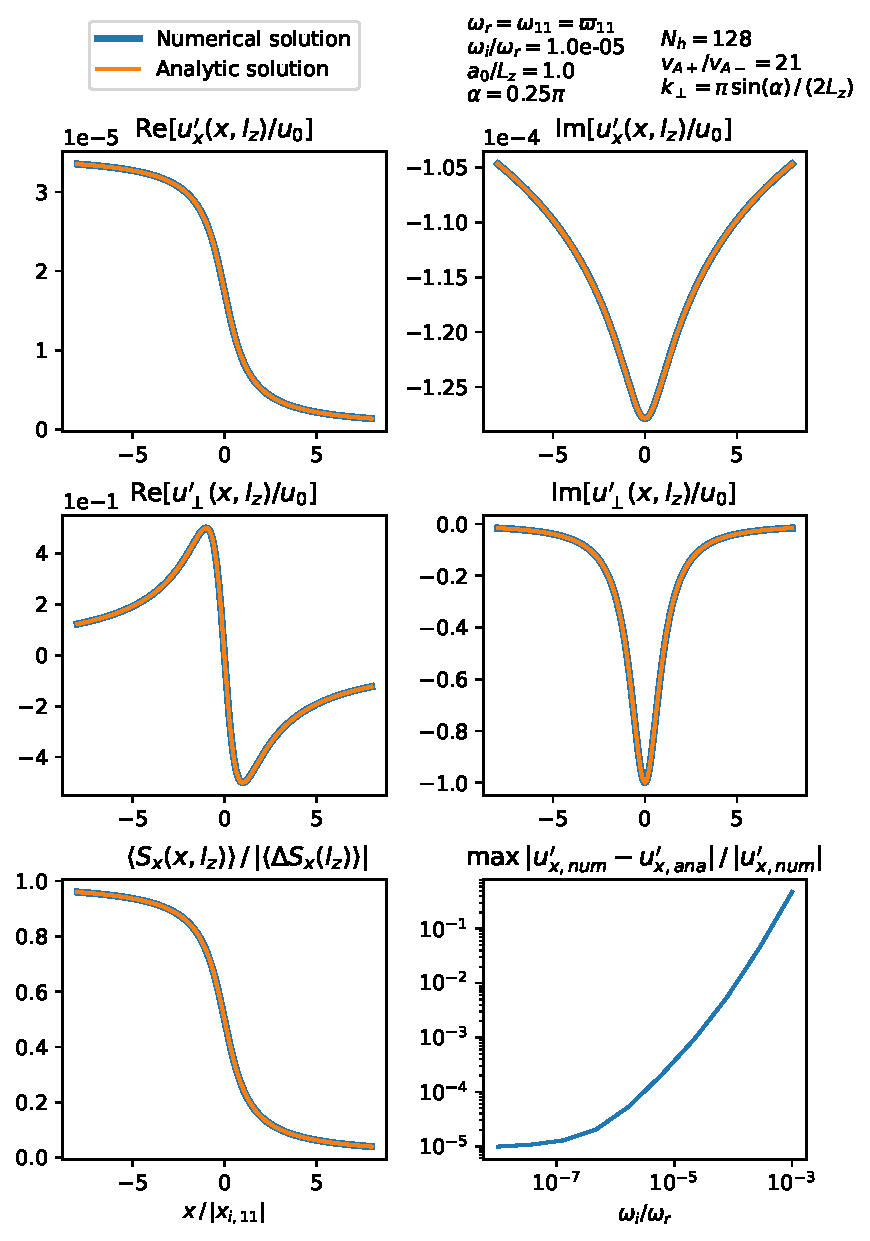
\includegraphics[width=\textwidth,height=0.8\textheight,keepaspectratio]{figures/chapter04/oblique_field_spectral_method_along_x.pdf}
    \vspace{-10pt}
    \caption{This figure shows plots of the real and imaginary parts of $u_x'$ (top row), $u_\perp'$ (middle row) and $\langle S_x' \rangle$ (bottom left) as a function of $x$ at $z=l_z$. We calculated the blue curves numerically and the orange curves plot Equations \eqref{eq:chap_4_oblique_u_perp_final}, \eqref{eq:chap_4_oblique_ux_final} and \eqref{eq:oblique_field_poy_flux_ana}. The bottom right plot shows the relative error between the numerical and analytic solutions for $u_x$ as a function of $\omega_i / \omega_r$. The velocity curves are normalised by $u_0$ which gives the amplitude of $u_\perp$ at $x=0$. The Poynting flux is normalised by $\abs{\langle \Delta S_x' \rangle}$ at $z=l_z$ (see Equation \eqref{eq:chap_4_jump_in_poy_flux}). The code used to make this figure is available on GitHub in the following directory:\newline
    \href{https://github.com/aleksyprok/apkp_thesis/blob/main/Python/Chapter4/spectral_code/line_along_x.py}{$\rightarrow$ Python/Chapter4/spectral\_code/line\_along\_x.py}}
    \label{fig:oblique_field_spectral_method_along_x}
    \vspace{-20pt}
\end{figure}

\begin{figure}
    \centering
    \vspace{-20pt}
    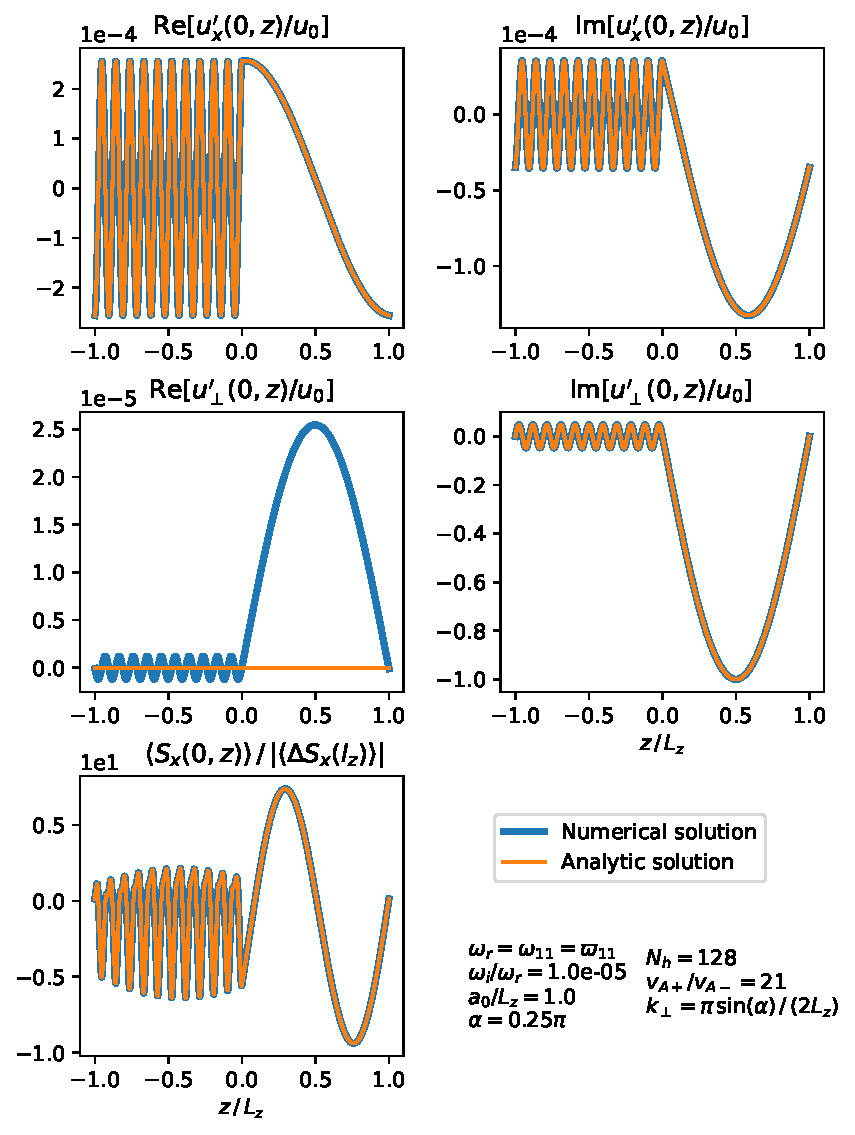
\includegraphics[width=\textwidth,height=0.9\textheight,keepaspectratio]{figures/chapter04/oblique_field_spectral_method_along_z.pdf}
    \vspace{-10pt}
    \caption{This figure is similar to Figure \ref{fig:oblique_field_spectral_method_along_x} except it plots the variables as function of $z$ at $x=0$ instead. The code used to make this figure is available on GitHub in the following directory:\newline
    \href{https://github.com/aleksyprok/apkp_thesis/blob/main/Python/Chapter4/spectral_code/line_along_z.py}{$\rightarrow$ Python/Chapter4/spectral\_code/line\_along\_z.py}}
    \label{fig:oblique_field_spectral_method_along_z}
    \vspace{-20pt}
\end{figure}

To check that the numerical solutions agree with the analytic solutions given by Equations \eqref{eq:chap_4_oblique_u_perp_final}, \eqref{eq:chap_4_oblique_ux_final} and \eqref{eq:oblique_field_poy_flux_ana} and to help visualise the solutions, we plot the solutions in Figure \ref{fig:oblique_field_spectral_method_along_x} and \ref{fig:oblique_field_spectral_method_along_z}. They show that the analytic and numerical solutions do agree provided $\omega_i/\omega_r$ is small enough. The bottom right of the Figure \ref{fig:oblique_field_spectral_method_along_x} shows the maximum relative error between the numerical and analytic solutions for $u_x$, which is given by
\begin{equation}
    \text{max relative $u_x'$ error} = \max_{\substack{-8|x_{i,11}|\le x\le 8|x_{i,11}| \\ -L_z\le z \le L_z}}\abs{\frac{u_{x,num}'-u_{x,ana}'}{u_{x,num}'}},
\end{equation}
where $u_{x,num}'$ denotes the $u_x'$ solution which was calculated numerically and $u_{x,ana}'$ was calculated analytically using Equation \eqref{eq:chap_4_oblique_ux_final}. The bottom right of the Figure \ref{fig:oblique_field_spectral_method_along_x} shows that decreasing $\omega_i/\omega_r$ causes the error to decrease. This plot appears to be converging to a non-zero value and this is because the numerical solution only uses a finite number of harmonics $N_h$. Increasing $N_h$ acts to reduce the error further. Figure \ref{fig:oblique_field_spectral_method_along_z} shows that although the amplitude of $u_\perp$ may decrease significantly in the chromosphere, this is not necessarily true for $u_x$. Equation \eqref{eq:oblique_field_uniform_in_x_ux10-} also shows that $u_x$ in the chromosphere will not necessarily go to zero, even if $v_{A-}\rightarrow0$. This suggests that imposing line-tied ($\vec{u}=0$) boundary conditions at the edge of the corona will lead to the generation of unphysical structures. The usual justification for imposing line-tied boundary conditions is that the chromosphere is significantly denser than the corona and so it acts like a solid wall. Here, $v_{A+}/v_{A-}=21$ and yet $u_x$ is showing no signs of going to zero in the chromosphere. Although $u_x$ does not go to zero, the kinetic energy and magnetic energy is dominated by $u_\perp$ and $b_\perp$, therefore, the kinetic and magnetic energy is approximately uniformly distributed along $z$.

\section{Summary and conclusions}
\label{sec:chap_4_conclusions}

The first results we presented in this chapter were shown in Section \ref{sec:chap_4_energy_equations}. We showed that oscillations in the $x$ and $\vec{\hat{B}}_0$ directions couple to the oscillations in the $\perp$ due to gradients in the magnetic pressure perturbation, $B_0b_{||}/(2\mu)$. Resonant absorption occurs where the mode conversion is one-way from fast wave perturbations to Alfv\'en waves. 

In Section \ref{sec:normal_field_resonant_absorption_with_line_tied_bcs} our goal was to introduce resonant absorption by using a model which was a simple as possible whilst complex enough to show some of its key properties. For simplicity, we chose the background magnetic field to be at right-angles to the $z=\text{constant}$ plane, i.e. $\alpha=0$ and the background Alfv\'en speed to be a function of just $x$. We calculated the normal mode solutions and derived a single ODE which $u_y$ satisfies, see Equation \eqref{eq:chap_4_uy_ode}. To solve the ODE we used method of Frobenius and showed that the solution can become singular at resonant locations $x_{res,n}$ where $\mathcal{L}_n(x_{res,n})=0$, i.e. at locations where the Alfv\'en wave equation is satisfied. This shows that resonant absorption occurs at locations where the frequency of the driver equals the natural Alfv\'en frequency of a field line. We calculated the leading order approximations of the singular solutions and verified these numerically via a graphical approach in Figure \ref{fig:normal_mode_along_x_alpha=0}.

In Section \ref{sec:oblique_field_uniform_density_profile_with_line_tied_bcs} we showed how Alfv\'en waves propagating from the corona to the chromosphere mode convert at the transition region to form fast waves. If
\[k_x \ge \Re\qty(\sqrt{k_{||0}^2 - k_y^2}),\]
then the fast waves are evanescent in the corona and will form boundary layers at the transition region (see Figures \ref{fig:piecewise_constant_vs_uniform_real_part} and \ref{fig:piecewise_constant_vs_uniform_imag_part}). This phenomenon has been shown in for example, \citet{Halberstadt1993,Halberstadt1995,Arregui2003}. 
To simulate the conditions near a singularity in a resonant absorption experiment, we calculated asymptotic expansions for $k_x / k_{||+} \rightarrow \infty$ (see Equations \ref{eq:chap_4_oblique_ux1}-\ref{eq:chap_4_oblique_b_par3}). They show that the boundary layers do not form if the magnetic field is normal to the transition region, i.e. if $\alpha=0$.

After that, we tested the validity of line-tied boundary conditions by checking if these boundary layers still form if a piecewise constant background Alfv\'en speed with continuity of $\vec{u}$ and $\dv*{\vec{u}}{z}$ is imposed instead (see Section \ref{sec:oblique_field_piecewise_constant_density_profile}). We believe we are the first authors to test line-tied boundary conditions in this way. The results (see Figures \ref{fig:piecewise_constant_vs_uniform_real_part}-\ref{fig:fast_wave_error_vs_kx}) suggest that line-tied boundary conditions provide a good approximation provided the fast waves can propagate in the chromosphere, i.e.
\[k_x \le \Re(\sqrt{k_{||-}^2 - k_y^2}).\]
However, if the fast waves are evanescent in the chromosphere, i.e. 
\[k_x \ge \Re(\sqrt{k_{||-}^2 - k_y^2}).\]
then line-tied boundary conditions will overestimate the size of the boundary layers by a factor of the order $k_x / k_{||-}$. If $k_x\gg k_{||-}$ then Equations \eqref{eq:oblique_field_uniform_in_x_ux10-}-\eqref{eq:oblique_field_uniform_in_x_b_par30+} approximate the solution, however, if $k_{||+} \ll k_x\ll k_{||-}$ then the line-tied solutions (Equations \ref{eq:chap_4_oblique_ux1}-\ref{eq:chap_4_oblique_b_par3}) provide a better approximation. We estimated that if the Alfv\'en waves are able to phase-mix to the shortest length scales allowed by the resistivity and viscosity in the corona then the $k_x\gg k_{||-}$ is usually most appropriate limit. However, during the early stages, before the waves have phase-mixed, $k_x\ll k_{||-}$ is the most valid limit.

The results from Section \ref{sec:oblique_field_piecewise_constant_density_profile} suggest that the fast wave component of the velocity should go to zero near singular locations in a resonant absorption experiment since $k_x\rightarrow \infty$ approaching the singularity. In the final section (Section \ref{sec:oblique_field_resonant_absorption}), we tested this by calculating the normal mode resonant absorption solution in a domain where the background Alfv\'en speed is a function of $x$ and piecewise constant in $z$. We used periodic boundary condition in $z$ for convenience and because this simulates a loop which goes from the corona to the chromosphere then back to the corona and so on. In Section \ref{sec:oblique_field_resonant_absorption_analytic_soln} we calculated the leading order singular solutions near a resonant location analytically. In Section \ref{fig:oblique_field_spectral_method_along_z} and \ref{fig:oblique_field_spectral_method_along_x} we plot the analytic and numerical solutions together and show that they agree. We verified that to leading order, $u_x$ and $u_\perp$ do not contain any boundary layers near the singularity. This confirms that imposing line-tied boundary conditions can cause the model to significantly overestimate the boundary layers' amplitude. However, in Section \ref{sec:oblique_field_piecewise_constant_density_profile} we showed as $k_x\rightarrow\infty$ the amplitude of the boundary layers does not increase. This suggests that the boundary layers have a limited effect on the rate at which the resonant absorption occurs. Moreover, since the boundary layers are evanescent, they cannot directly transport energy away.

In conclusion, Alfv\'en waves will (in general) mode convert to form fast waves at the transition region. The fast waves can be evanescent or can propagate depending on the value of $\vec{k}\vdot\vec{k} - \omega^2$. We have demonstrated that line-tied boundary conditions can be more problematic than many authors realise. If $k_x$ grows large enough such that it causes the fast waves in the chromosome to be evanescent, then the line-tied model will fail to reduce the boundary layer's size accurately. We believe that few authors are aware of this because it is quite counter-intuitive that $k_x$ (which gives the length-scales in a direction tangential to the chromosphere/corona interface) can be important in determining the validity of line-tied boundary conditions. Increasing $k_x$ can result in the line-tied model greatly overestimating the boundary layer's amplitude by approximately a factor $k_x / k_{||-}$. With that in mind, we believe authors should continue to use line-tied boundary conditions for their simplicity and ability to reduce computation time, provided that their flaws are understood. For example, we have shown that line-tied boundary conditions provide a good approximation (with an error of the order $v_{A-}/v_{A+}$) if the fast waves can propagate in the chromosphere. If the fast waves are evanescent in the chromosphere, then line-tied boundary conditions are less useful. However, sometimes this won't be important. For example, when studying energetics, as the boundary layers are evanescent and cannot transport energy away. Moreover, we showed in Section \ref{sec:oblique_field_uniform_density_profile_with_line_tied_bcs} that their energy does not grow as $k_x\rightarrow \infty$.

% The primary aim of this chapter is to test if line-tied boundary conditions cause unphysically large boundary layers/evanescent fast waves to form in resonant absorption experiments. To test this, Section \ref{sec:oblique_field_uniform_density_profile_with_line_tied_bcs} calculated the solutions with line-tied boundary conditions imposed and Section \ref{sec:oblique_field_piecewise_constant_density_profile} calculated the solutions with the chromosphere included in the model instead. We compared results from both sections and found that the boundary layers only appear in the leading order solution for $u_x$ in the model with line-tied boundary conditions, they are absent if the chromosphere is included.
% This shows that imposing line-tied boundary condition causes the model to overestimate significantly the amplitude of the evanescent fast waves/boundary layers. Note that Sections \ref{sec:oblique_field_uniform_density_profile_with_line_tied_bcs} and \ref{sec:oblique_field_piecewise_constant_density_profile} used a background Alfv\'en speed which did not depend on $x$ so resonant absorption could not occur. However, we simulated the conditions near a singularity in a resonant absorption experiment by imposing very short length scales in $x$. To help verify the conclusions made from Section \ref{sec:oblique_field_uniform_density_profile_with_line_tied_bcs} and \ref{sec:oblique_field_piecewise_constant_density_profile} we used an Alfv\'en speed which depended on $x$ in Section \ref{sec:oblique_field_resonant_absorption}. This enabled resonant absorption to occur and we confirmed that near the singularity the boundary layers are absent in the solution for $u_x$ and $u_\perp$ to leading order. We believe line-tied boundary conditions are useful for their simplicity and convenience, provided their flaws and limitations are understood.

% Section \ref{sec:chap_4_energy_equations} showed that oscillations in the $x$ and $\vec{\hat{B}}_0$ directions couple to the oscillations in the $\perp$ due to gradients in the magnetic pressure perturbation, $B_0b_{||}/(2\mu)$. Resonant absorption occurs where the mode conversion is one-way from fast wave perturbations to Alfv\'en waves. 

% In Section \ref{sec:normal_field_resonant_absorption_with_line_tied_bcs} our goal was to introduce resonant absorption by using a model which was a simple as possible whilst complex enough to show some of its key properties. For simplicity, we chose the background magnetic field to be at right-angles to the $z=\text{constant}$ plane, i.e. $\alpha=0$ and the background Alfv\'en speed to be a function of just $x$. We calculated the normal mode solutions and derived a single ODE which $u_y$ satisfies, see Equation \eqref{eq:chap_4_uy_ode}. To solve the ODE we used method of Frobenius and showed that the solution can become singular at resonant locations $x_{res,n}$ where $\mathcal{L}_n(x_{res,n})=0$, i.e. at locations where the Alfv\'en wave equation is satisfied. This shows that resonant absorption occurs at locations where the frequency of the driver equals the natural Alfv\'en frequency of a field line. We calculated the leading order approximations of the singular solutions and verified these numerically via a graphical approach in Figure \ref{fig:normal_mode_along_x_alpha=0}.

% In Section \ref{sec:oblique_field_uniform_density_profile_with_line_tied_bcs} we used a uniform background Alfv\'en speed and imposed line-tied boundary conditions at $z=0$. We imposed an incident Alfv\'en wave from $z>0$ and calculated the unique solution which ensures $u_x=u_\perp=0$ at $z=0$. After that, we calculated asymptotic expansions for the solution, see Equations \eqref{eq:chap_4_oblique_ux1}-\eqref{eq:chap_4_oblique_b_par3} for $k_x\rightarrow\infty$. We solve for the large $k_x$ limit as this simulates the singularities which form in resonant absorption experiments. Equations \eqref{eq:chap_4_oblique_ux1}-\eqref{eq:chap_4_oblique_ux3} show that $u_x$ contains an evanescent fast wave/boundary layer term to leading order. This is in agreement with similar results found in, for example, \citet{Halberstadt1993,Halberstadt1995,Arregui2003}. Note that the fast wave terms go to zero if $\alpha=0$, i.e. if the background magnetic field is perpendicular to the transition region.

% Section \ref{sec:oblique_field_piecewise_constant_density_profile} used a similar model to Section \ref{sec:oblique_field_uniform_density_profile_with_line_tied_bcs} except the Alfv\'en speed was piecewise constant in $z$ instead of uniform. We imposed an incident Alfv\'en wave from $z>0$ and calculated the unique solution which ensures continuity of $u_x$, $u_\perp$, $\pdv*{u_x}{z}$, $\pdv*{u_\perp}{z}$ at $z=0$. After that, we calculated asymptotic expansions for the solution, see Equations \eqref{eq:oblique_field_uniform_in_x_ux10-}-\eqref{eq:oblique_field_uniform_in_x_b_par30+} for $k_x\rightarrow\infty$. They show that fast wave terms are negligible in $u_x$ and $u_\perp$ to leading order. Compare this with Section \ref{sec:oblique_field_uniform_density_profile_with_line_tied_bcs} which showed that the solution for $u_x$ contains a boundary layer term to leading order. Therefore, imposing line-tied boundary conditions can cause the model to overestimate significantly the boundary layers to leading order and we believe we are the first authors to demonstrate this. 
% % For the asymptotic series to be valid, we showed that Equation \eqref{eq:chap_4_kx_condition} needs to be satisfied. Hence, for finite $k_x$, if $v_{A-}\rightarrow0$, then the boundary layer terms can be of equal order to the Alfv\'en wave terms in $u_\perp$. 
% % However, in a resonant absorption experiment, near the singularity, $k_x\rightarrow \infty$ causing Equation \eqref{eq:chap_4_kx_condition} to be satisfied for any non-zero $v_{A-}$.

% Finally, section \ref{sec:normal_field_resonant_absorption_with_line_tied_bcs} aimed to check that $u_x$ and $u_\perp$ contain no boundary layer terms to leading order in resonant absorption experiments. The Alfv\'en speed was piecewise constant in $z$ and dependent on $x$. We imposed periodic boundary conditions for convenience and to ensure the solution is unique. These boundary conditions model a loop which goes through the corona, into the chromosphere, back into the corona and so on. In Section \ref{sec:oblique_field_resonant_absorption_analytic_soln} we calculated the leading order singular solutions near a resonant location analytically. Section \ref{sec:oblique_field_resonant_absorption_numerical_soln} verified the analytic solutions using eigenfunctions to convert the PDEs into a set of ODEs which we solved numerically. Figures \ref{fig:oblique_field_spectral_method_along_x} and \ref{fig:oblique_field_spectral_method_along_z} plot the analytic and numerical solutions side-by-side and show that they agree. We verified that the boundary layers terms are absent in the leading order solution for $u_x$ and $u_\perp$ near the singularity and this confirms that imposing line-tied boundary conditions causes the model to overestimate significantly the amplitude of the boundary layers. However, in Section \ref{sec:oblique_field_uniform_density_profile_with_line_tied_bcs} we showed as $k_x\rightarrow\infty$ the amplitude of the boundary layers does not increase. This suggests that the boundary layers have a limited effect on the rate at which the resonant absorption occurs. Moreover, since the boundary layers are evanescent, they cannot directly transport energy away.